\documentclass[a4paper,twoside,openright,11pt,oldfontcommands]{memoir}

\usepackage[pdftex,hyperindex,bookmarks,linktoc=all]{hyperref}

\let\printglossary\relax
\let\theglossary\relax
\let\endtheglossary\relax
\usepackage[acronym,toc,nomain]{glossaries}
\makeglossaries

\usepackage[australian]{babel}
\usepackage[english=british]{csquotes}
\usepackage[bf,sf]{titlesec}

% fix a bug in titlesec
\makeatletter
\patchcmd{\ttlh@hang}{\parindent\z@}{\parindent\z@\leavevmode}{}{}
\patchcmd{\ttlh@hang}{\noindent}{}{}{}
\makeatother


\usepackage{microtype}
\usepackage{algorithm}
\usepackage[dvipsnames,table,xcdraw]{xcolor}

% UNSW margin guidelines:
%
%   Top >= 30mm
%   Bottom >= 20mm
%   Left >= 40mm (do they mean inner?)
%   Right >= 20mm (do they mean outer?)
%
\usepackage[
        inner=36mm, % NOPRINT
        outer=36mm, % NOPRINT
        top=30mm,
        bottom=35mm,
        headsep=10mm,
        headheight=20pt,
        footskip=12mm,
        includehead=false,
        includefoot=false,
        marginparwidth=30mm,
        heightrounded=true
        ]{geometry}

\frenchspacing

% font
\usepackage{amsfonts}
\usepackage[tt=false,type1=true]{libertine}
\usepackage{inconsolata}
\usepackage[T1]{fontenc}
\renewcommand\cftappendixname{\appendixname~}
\usepackage[normalem]{ulem} % provides \sout and \xout for strikethrough text

% graphics are in imgs/ dir
\usepackage[pdftex]{graphicx}
\graphicspath{{imgs/}}

\usepackage{mwe}
\usepackage{setspace}
\usepackage{datetime}
\newdateformat{monthyear}{\monthname[\THEMONTH] \THEYEAR}

% maths
\usepackage{amssymb}
\usepackage{amsmath}
\usepackage{pifont}
\usepackage{textcomp}
\usepackage{gensymb}
\usepackage{mathptmx}
\hypersetup{
    pdfborder = {0 0 0.75 [1.5 3]},
    allbordercolors = {0.122 0.471 0.706},
    colorlinks,
    citecolor=black,
    filecolor=black,
    linkcolor=black,
    urlcolor=black
    }
% references
%  use \cref to reference labels and automagically guess the
% name (ie Section, Figure etc).
\usepackage[capitalise]{cleveref} 


% code - note you need to install pygmentize (sudo apt-get install python-pygments)
% and invoke pdflatex as follows: pdflatex -shell-escape phd.tex
\usepackage[newfloat=true]{minted}
\usemintedstyle{borland}

% captions
\usepackage{caption}
\captionsetup{font=small,format=hang,position=below} % format=hang,
\captionsetup[listing]{font=small,format=hang,position=below} % format=hang,
\usepackage{subcaption}

\usepackage{array}
\usepackage{pdfpages}

% tables
\usepackage{colortbl} % be able to colour rows in tables
\usepackage{tabularx} % use tabularx to specify width of table, X is a column to fill width of table
\usepackage{multirow} % supports rows spanning multiple cells
\setlength{\extrarowheight}{3pt} % increase table row height
\newcommand{\tableheadline}[1]{\multicolumn{1}{l}{\spacedlowsmallcaps{#1}}}
% reset rowcolor after every table -- required so tabularx and rowcolor behave
\newcounter{tblerows}
\expandafter\let\csname c@tblerows\endcsname\rownum
\usepackage{booktabs} % pretty book style tables

% abbreviations with correct spacing
\usepackage{xspace}
\newcommand*{\eg}{e.g.\@\xspace}
\newcommand*{\ie}{i.e.\@\xspace}
\newcommand*{\IO}{I/O\@\xspace}
\makeatletter
\newcommand*{\etc}{%
    \@ifnextchar{.}%
                {etc}%
                {etc.\@\xspace}%
}
\makeatother

% lists 
\usepackage{enumitem}
\setlist[enumerate]{itemsep=0mm}
\setlist[itemize]{itemsep=0mm}

\usepackage{verbatim}
\usepackage{pgfgantt}
\usepackage{pgfplots}
\usepackage{chngpage}
\pgfplotsset{width=7cm,compat=newest}
\usepackage{url}
% allow latex to break urls up over lines
\Urlmuskip=0mu plus 1mu

% bibliography
\usepackage[authoryear,square,sort]{natbib}
\usepackage{bibentry}
\renewcommand{\cite}{\citep}
\usepgfplotslibrary{ternary}
\newif \ifDraft        \Drafttrue

% short cut for tick and cross commands
\newcommand{\yes}{\checkmark}
\newcommand{\no}{\hspace{1pt}\ding{55}}

% sel4 system call shortcuts
\newcommand{\code}[1]{\texttt{#1}\xspace}
\newcommand{\call}{\code{call}}
\newcommand{\send}{\code{send}}
\newcommand{\nbsend}{\code{nbsend}}
\newcommand{\wait}{\code{wait}}
\newcommand{\nbwait}{\code{nbwait}}
\newcommand{\recv}{\code{recv}}
\newcommand{\nbrecv}{\code{nbrecv}}
\newcommand{\reply}{\code{reply}}
\newcommand{\replyrecv}{\code{replyrecv}}
\newcommand{\yield}{\code{yield}}
\newcommand{\nbsendwait} {\code{nbsendwait}}
\newcommand{\nbsendrecv} {\code{nbsendrecv}}
\newcommand{\sendrecv} {\code{sendrecv}}


\newcommand{\selfour}{seL4\xspace} % use as normal text, examples below.
\newcommand{\hires}{\textsc{HiRes}\xspace}
\newcommand{\litmus}{\textsc{litmus\textsuperscript{RT}}\xspace}
\newcommand{\flare}{FlaRe\xspace}
\newcommand{\fiascooc}{Fiasco.OC\xspace}
\newcommand{\composite}{\textsc{Composite}\xspace}
\newcommand{\minix}{\textsc{Minix 3}\xspace}
\newcommand{\linuxrk}{Linux/RK\xspace}

\newcommand{\schedfifo}{\texttt{SCHED\_FIFO}\xspace}
\newcommand{\schedrr}{\texttt{SCHED\_RR}\xspace}
\newcommand{\schedsporadic}{\texttt{SCHED\_SPORADIC}\xspace}
\newcommand{\noprioinherit}{\texttt{NO\_PRIO\_INHERIT}\xspace}
\newcommand{\prioinherit}{\texttt{PRIO\_INHERIT}\xspace}
\newcommand{\prioprotect}{\texttt{PRIO\_PROTECT}\xspace}

\newcommand{\crit}[1]{\textsc{#1}\xspace}
% Leave this in here, it is often useful to deal with latexdiff breakage.
% Put it around breakage-causing segments (in both versions to be diffed!)
\newenvironment{DIFnomarkup}{}{}

\urlstyle{rm}

\newcolumntype{i}[1]{%
    >{
\itemize[leftmargin=0.3cm]}
			p{#1}%
		<{\enditemize}}

\newcommand{\itemcol}[1] {
		\multicolumn{1}{i{5cm}|}{#1}
}

% TODOS 
\newcommand{\TODO}[1]{\textbf{\textsl{TODO: #1}}}

%
% Footnote styling.
%

% 10pt footnotes, per requirements
\renewcommand{\footnotesize}{\fontsize{9}{10}\selectfont}

% Frown upon splitting footnotes.
\interfootnotelinepenalty=5000

% Allow a bit of stretching at the bottom of the y neccessary.
%\makeatletter
%\def\@textbottom{\vskip\z@\@plus.1pt}
%\let\@texttop\relax
%\makeatother

\title{Mixed-Criticality Scheduling 
      and Resource Sharing for
     High-Assurance Operating Systems}
\author{Anna Lyons}
%\AuthorEmail{Anna.Lyons@data61.csiro.au}


% chapter headings

%make our pretty chapter headings
% Copied from AlexL via DaveC via Adam
\newcommand{\chapformat}[1]{\parbox[c]{0.8\textwidth}{\Huge #1}}
\titleformat{\chapter}[hang]
    {\bfseries}
    {\parbox[c]{0.2\textwidth}{\rmfamily\fontsize{72}{72}
     \selectfont\thechapter\hspace{10pt}\rule[-12pt]{2pt}{72pt}}}
    {0pt}
    {\chapformat}
    []


\setsecnumdepth{subsubsection}

\widowpenalty10000
\clubpenalty10000

% evaluation commands
\newcommand{\inputbenchmarkrows}[3]{
    \midrule
    \multirow{2}{*}{\textsc{#1}}
    \input{data/generated/#2-#3-micro.inc}
}

\newcommand{\ipcmicro}[3]{\inputbenchmarkrows{#1}{#2}{#3-ipc}}
\newcommand{\faultmicro}[2]{\inputbenchmarkrows{#1}{#2}{fault}}
\newcommand{\irqmicro}[2]{\inputbenchmarkrows{#1}{#2}{irq}}
\newcommand{\schedulemicro}[2]{\inputbenchmarkrows{#1}{#2}{schedule}}

\input{glossary}
\begin{document}

% code style
\setminted{baselinestretch=1.2,frame=lines,fontsize=\footnotesize,linenos,framesep=3mm,xleftmargin=3mm,xrightmargin=3mm,breaklines,breakautoindent,tabsize=2}
\setmintedinline{breaklines}


% tell latex this is the preamble
\frontmatter
% Title page 
%% Title page
%\newgeometry{margin=1mm,left=1cm}
%\begin{titlepage}

\frontmatter
\thispagestyle{empty}
\calccentering{\unitlength}                         % Calculate center length and stores in unitlength
\begin{adjustwidth*}{\unitlength}{-\unitlength}     % Adjust center
    \begin{adjustwidth}{-1cm}{-1cm}                 % Extra lage front page

\mbox{}
\vfill
\begin{center}
    {\Huge\sffamily\bfseries Mixed-Criticality Scheduling and Resource Sharing for High-Assurance Operating Systems\\[1cm]\par}
{\Large\sffamily\bfseries Anna Lyons}\\[1.5cm]
Submitted in fulfilment of the requirements for the degree of \\
Doctor of Philosophy\\[1cm]
\includegraphics[width=0.32\linewidth]{unicrest-colour} \\[1cm]
School of Computer Science and Engineering \\[0.5cm]
University of New South Wales \\[0.5cm]
Sydney, Australia \\[1.0cm]
\monthyear\today
\end{center}
\par
\vfill

\end{adjustwidth}
\end{adjustwidth*}
%\end{titlepage}
%\restoregeometry

\cleardoublepage

%
\includepdf{thesisdissertation_sheet.pdf}
%\cleardoublepage

%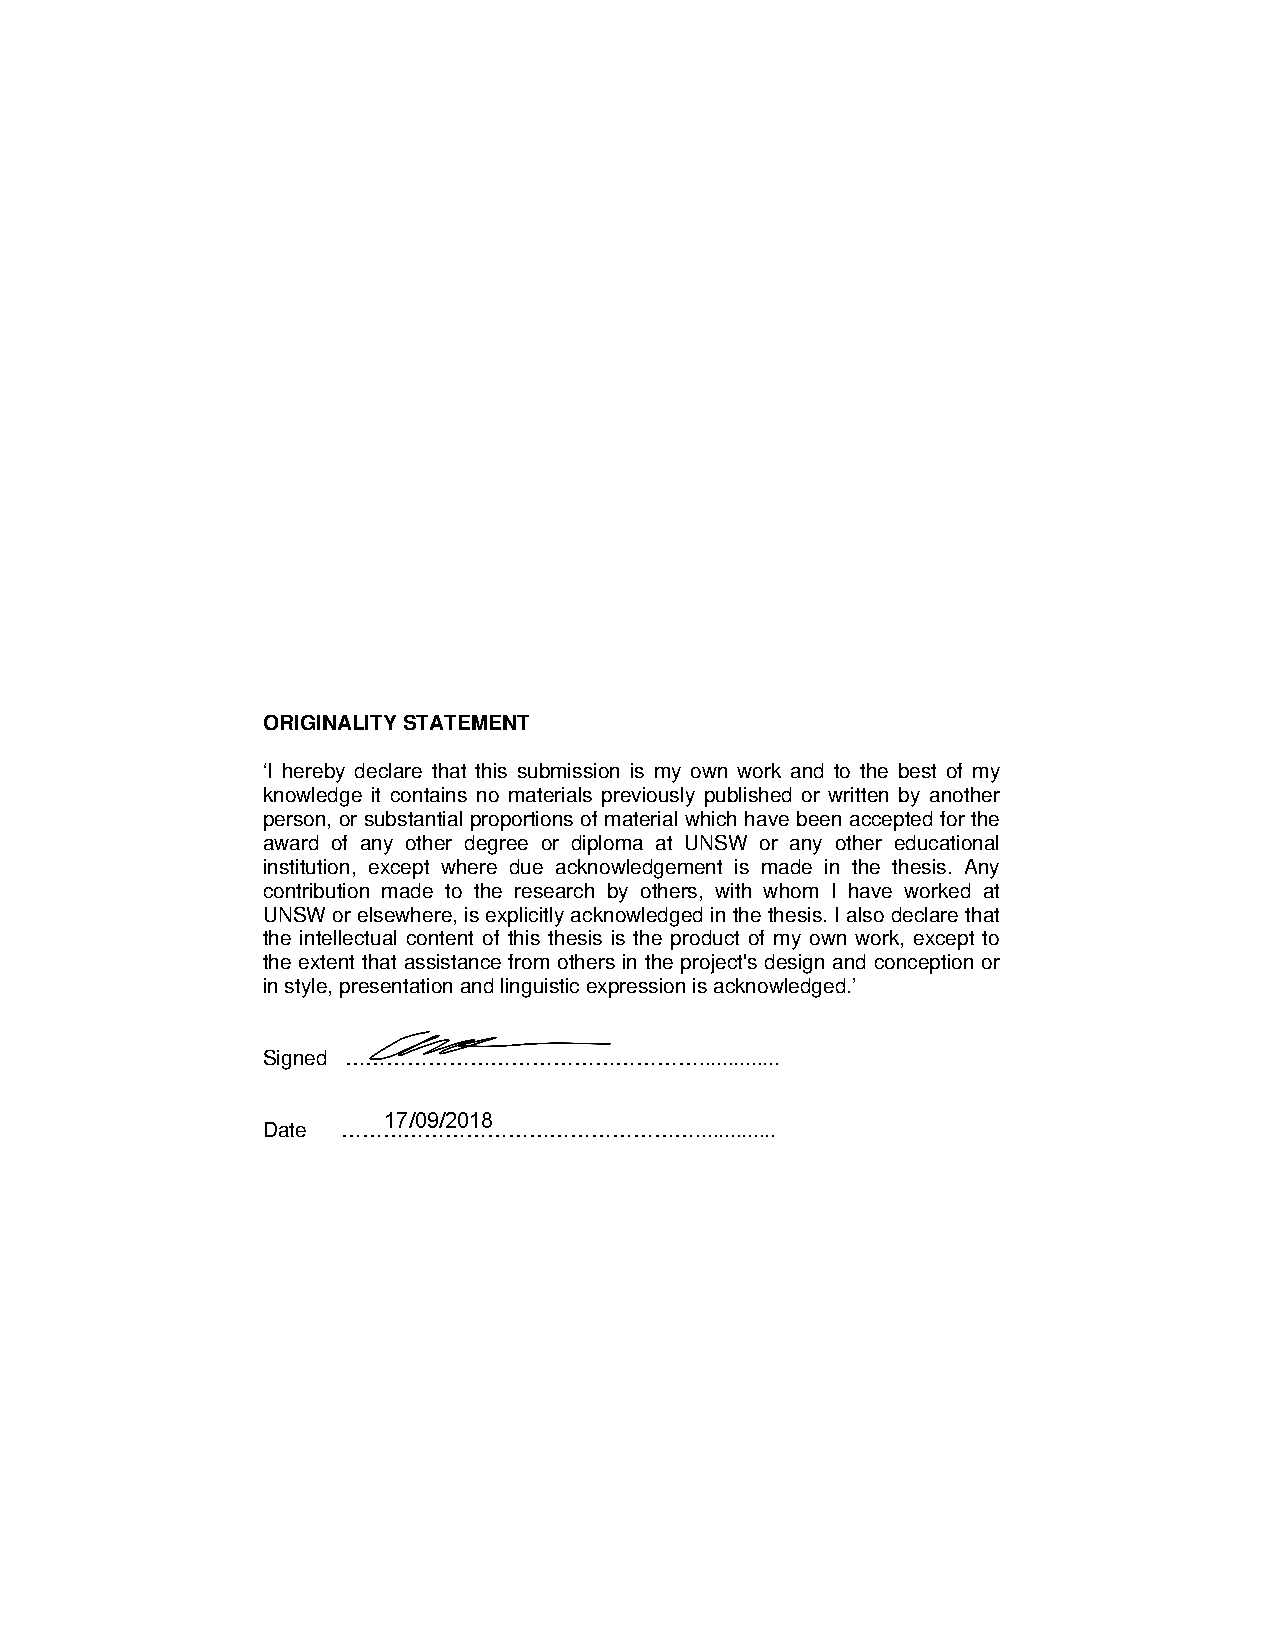
\includepdf{originalitystatement.pdf}
%\cleardoublepage

%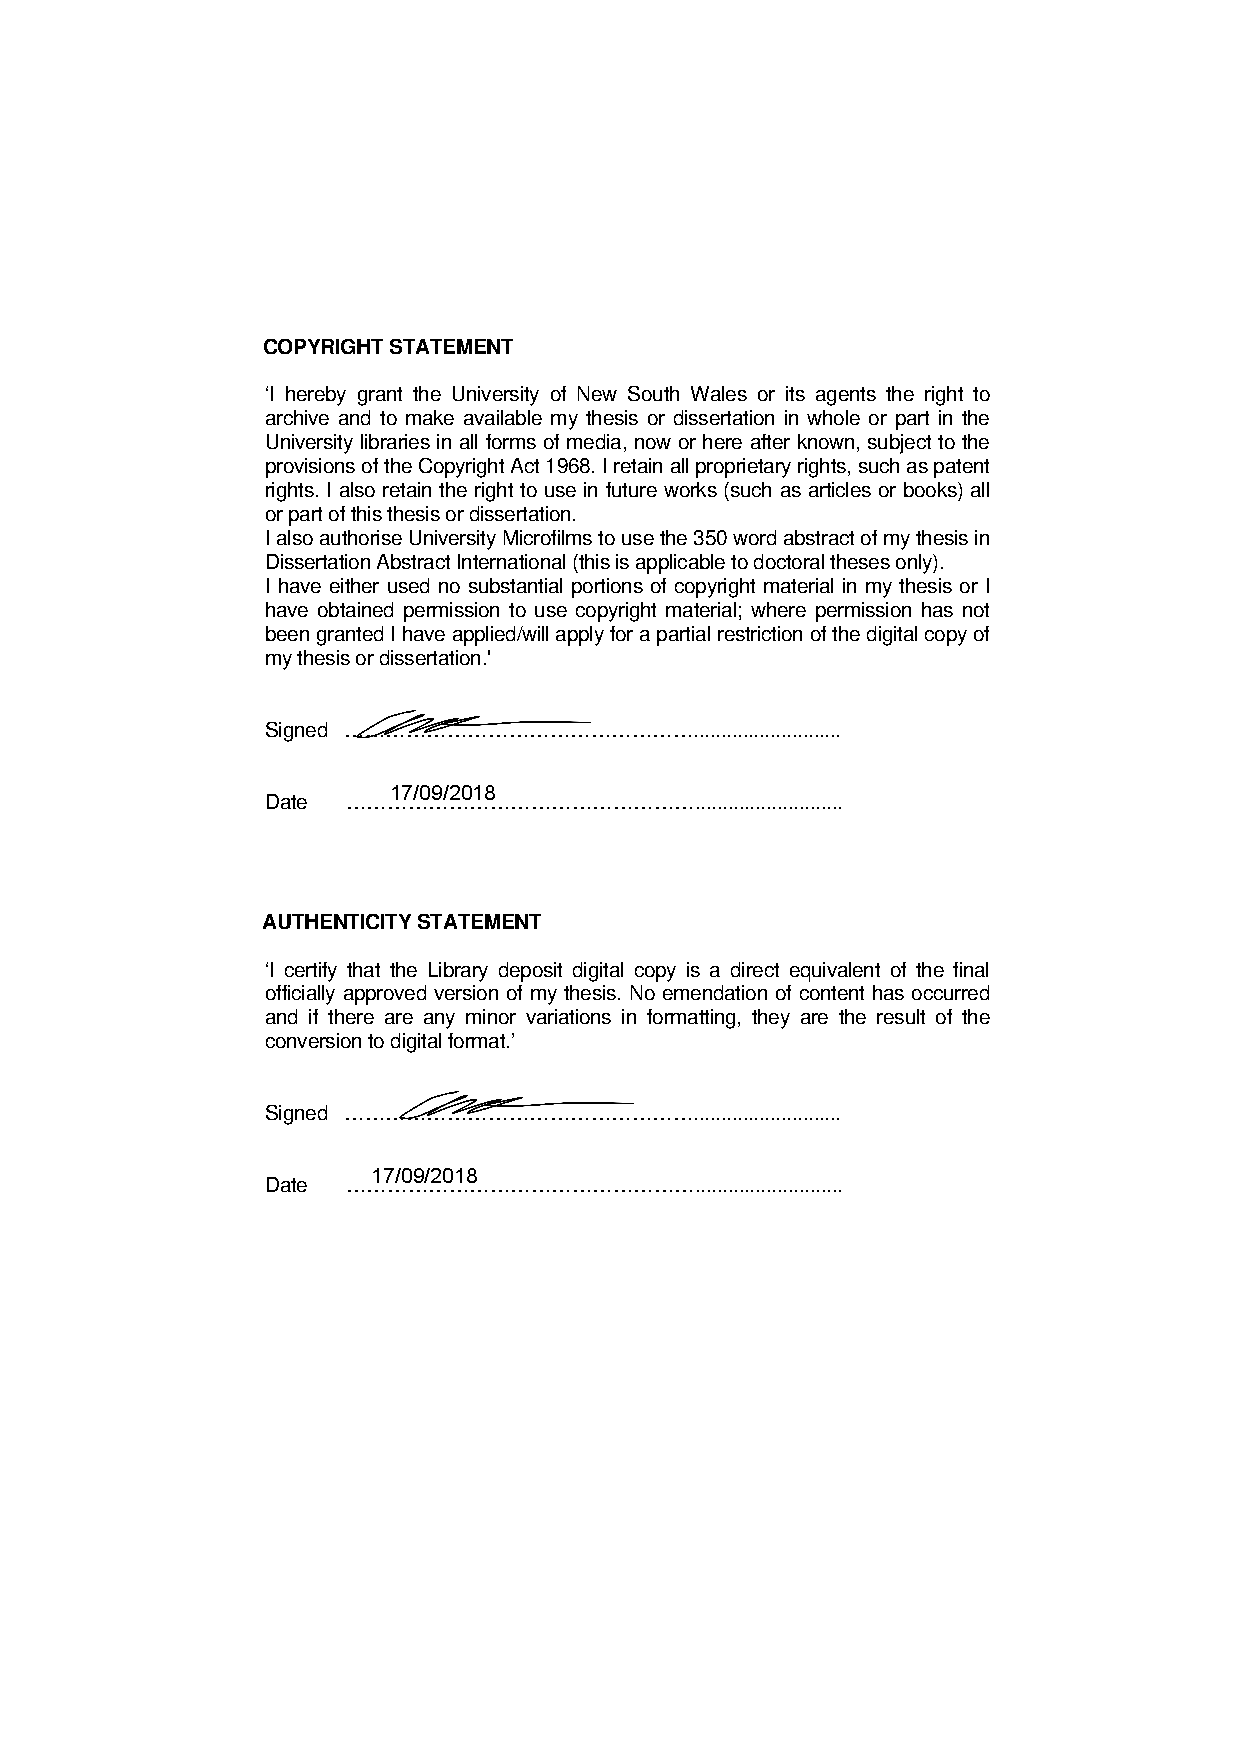
\includepdf{copyrightauthenticitystatements_0}
%\cleardoublepage


\urlstyle{sf}
\pagestyle{plain}

%Abstract

\begin{abstract}
Criticality of a software system refers to the severity of the impact of a failure.
In a high-criticality system, failure risks significant loss of life or damage to the environment.
In a low-criticality system, failure may risk a downgrade in user-experience.
As criticality of a software system increases, so too does the cost and time to develop that
software: raising the criticality also raises the assurance level, with the highest levels requiring
extensive, expensive, independent certification.

For modern cyber-physical systems, including autonomous aircraft and other vehicles, the traditional
approach of isolating systems of different criticality by using completely separate physical
hardware, is no
longer practical, being both restrictive and inefficient.
The result is \emph{mixed-criticality} systems, where software applications with different criticalities
execute on the same hardware. Sufficient mechanisms are required to ascertain that software in
mixed-criticality systems  is sufficiently isolated, otherwise, all software on that hardware is promoted
to the highest criticality level, driving up costs to impractical levels. For mixed-criticality systems to be
viable, both spatial and temporal isolation are required.

Current aviation standards allow for mixed-criticality systems where temporal and spatial resources
are strictly and statically partitioned in time and space, allowing some improvement over 
fully isolated hardware. However, further improvements are not only possible, but required for future
innovation in cyber-physical systems. 

This thesis explores further operating systems mechanisms to allow for mixed-criticality
software to share resources in far less restrictive ways, opening further possibilities in
cyber-physical system design without sacrificing assurance properties. 
Two key properties are required: first, time must be managed as a central resource of the system, while allowing for overbooking with asymmetric protection without increasing certification burdens.
Second, components of different criticalities should be able to safely share resources without suffering undue utilisation penalties.

We present a
model for capability-controlled access to processing time without incurring over-head related capacity loss or
restricting user policy, including processing time in shared resources. This is achieved by
combining the idea of resource reservations, from resource kernels, with the concept of resource
overbooking, which is central to policy freedom. The
result is the core mechanisms of scheduling contexts, scheduling context donation over IPC, and
timeout exceptions which allow  system designers to designate their own resource allocation policies.

We follow with an
implementation of the model in the \selfour microkernel, a high-assurance, high-performance platform.
Our final contribution is a thorough evaluation, including microbenchmarks, whole system benchmarks,
and isolation benchmarks. The micro- and system benchmarks show that our implementation is low
overhead, while the user-level scheduling benchmark demonstrates policy freedom in terms of
scheduling is retained. Finally, our isolation benchmarks show that our processor temporal isolation
mechanisms are effective, even in the case of shared resources.

\end{abstract}
\addcontentsline{toc}{chapter}{Abstract}
\clearpage

\clearpage
\input{acknowledgements}
\clearpage
\input{publications}
%\clearpage
%\listoffigures
%\clearpage
%\listoftables
%\clearpage
% glossary
\printglossary[type=\acronymtype]
%\clearpage


\cleardoublepage
\tableofcontents
% Somehow the clear double page, newpage, and pagebreak below here result in the intro chapter on the very next page
% From the table of contents
\cleardoublepage
\newpage

% tell latex to start the real page numbers
\mainmatter

\sloppy
\pagebreak

\chapter{Introduction}

% what is criticality
\emph{Criticality} of a software system refers to the severity of the impact of a failure.  In a
high-criticality system, failure risks significant loss of life or damage to the environment.  In a
low-criticality system, failure may risk a downgrade in user-experience.  Traditionally, systems of
different criticality were isolated by hardware.  This approach is no longer practical as it has
proven inefficient and restrictive.  The result is \emph{mixed-criticality} systems, where software
applications with different criticalities execute on the same hardware.
% Does a software application have mixed-criticality components or single criticality.
% Application, system, functional componet ?
% introduce challenges, example
However, mixed-criticality systems have conflicting requirements that challenge \glspl{OS} design:
they require mutually distrusting components of different criticalities to share resources and must
degrade gracefully in the face of failure.  For example, an \gls{AAV} has multiple inputs to its
flight-control algorithm: object detection, to avoid flying into obstacles, and navigation, to get
to the desired destination.  Clearly the object detection is more critical than navigation, as
failure of the former can be catastrophic, while the latter would only result in a non-ideal route.
Yet the two subsystems must cooperate, accessing and modifying shared data, thus cannot be fully
isolated.

The \gls{AAV} is an example of a mixed-criticality system, a notion that originates in avionics and its
need to reduce \gls{SWaP}, by consolidating growing functionality onto a smaller
number of physical processors. More recently the
\gls{MCAR}\citep{Barhorst_BBHPSSSSU_09} program was launched, which recognises that in order to
construct fully autonomous systems, critical and less critical systems must be able to share
resources. However, resource sharing between components of mixed-criticality is heavily restricted by current
standards.
% Non-fungibility of time,
% Difficulty in calculating wcet of high critical tasks -> overbooking.
% Varying processor time requirements of all tasks -> overbooking.
% what's wrong with static partitioning
While MCS are becoming the norm in avionics, this is presently in a very restricted form: the system
is orthogonally partitioned spatially and temporally, and partitions are scheduled with fixed time
slices~\citep{ARINC653}. Any components that share resources are promoted to the highest criticality
level and must meet the same certification standards; in other words, a critical component must not
trust a lower criticality one to behave correctly. This limits integration and cross-partition
communication, and implies long interrupt latencies and poor resource utilisation. 
% not just planes
These challenges are not unique to avionics: top-end cars exceeded 70 processors ten years
ago~\citep{Broy_KPS_07}; with the robust packaging and wiring required for vehicle electronics, the
SWaP problem is obvious, and will be magnified by the move to more autonomous operation. Other
classes of cyber-physical systems, such as smart factories, will experience similar challenges.

% more than consolidation
However, mixed-criticality systems are about more than basic consolidation; they can achieve more
than traditional physically isolated systems. Allowing untrusted, less critical components to
share hardware and communicate with more critical components, far more complex software can be
introduced to the system. Examples include heuristic algorithms that are common in artificial
% algorithms algorithms
intelligence algorithms, or internet connected software which by its nature cannot be completely
trusted. Both of these use-cases are far too complex to certify to the highest criticality standard,
but are essential for emerging cyber-physical systems like self-driving cars.

% finally, overcommitting
Our goal is to design and implement an OS that provides the right mechanisms for efficiently
supporting mixed criticality systems, and to reason about their safety.
The implementation platform will be the \selfour~\citep{Klein_EHACDEEKNSTW_09}
microkernel, which is has been designed for the high-assurance, safety-critical domain.

Concisely, the goals of this research are to provide:
\begin{enumerate}[label=\textbf{G\arabic*}] 
    \item\label{G1} A principled approach to
    processor management, treating time as a fundamental kernel resource, while
    allowing it to be overbooked, a key requirement of mixed-criticality systems;
    \item safe resource sharing between applications of different criticalities and
    different temporal requirements.  
\end{enumerate}


\section{Motivation}

% expand on notion of criticality with more detail and examples. Give enough background to justify contributions.
As noted in the introduction, the \emph{criticality} of a system reflects the
severity of failure, where higher criticality implies higher severity.  Table
\ref{tab:criticality_table} shows criticality levels considered when designing
software for commercial aircraft in the United States.

\begin{table}
     \centering
     \rowcolors{2}{gray!25}{}
     \begin{tabular}{ l p{10cm}} \toprule
         \emph{Level}   & \emph{Impact} \\ \midrule
         Catastrophic   & Failure may cause multiple fatalities, usually with loss of the airplane. \\
         Hazardous      & Failure has a large negative impact on safety or performance, or reduces the
                          ability of the crew to operate the aircraft due to physical distress or 
                          a higher workload, or causes serious or fatal injuries among the passengers.\\
         Major          & Failure significantly reduces the safety margin or significantly increases
                          crew workload. May result in passenger discomfort (or even minor
                          injuries).\\
         Minor          & Failure slightly reduces the safety margin or slightly increases crew
                          workload. Examples might include causing passenger inconvenience or a
                          routine flight plan change. \\
         No Effect      & Failure has no impact on safety, aircraft operation or crew workload. \\
         \bottomrule
     \end{tabular}
     \caption{Criticality levels from DO-178C, a safety standard for commercial aircraft.}
     \label{tab:criticality_table}
 \end{table}

% TODO are there any citations on cost per line of code?
Higher engineering and safety standards are required for higher criticality levels, up to
certification by independent certificate authorities at the highest levels. As a result, highly
critical software is incredibly expensive to develop and tends to have low complexity in order to
minimise costs. Any software that is not fully isolated from a critical component is promoted to
that level of criticality, increasing the production cost.

Traditionally, systems of different criticality levels were fully isolated with
air gaps between physical components. However, given the increased amount of
computing in every part of our daily lives, the practice of physical isolation
has resulted in unscalable growth in the amount of computing hardware in
embedded systems, with some modern cars containing over 100
processors~\citep{Hergenhan_Heiser_08}. The practise of physical separation is no 
longer viable for three reasons: \gls{SWaP}, efficiency, and function.

\paragraph{SWaP} First, systems with air-gaps require increased physical
resources: increasing production costs and environmental impact.
For vehicles, especially aircraft, this goes further to reduce their function; the
heavier the system,  the more fuel it requires to travel. This in turn reduces
utility in the form of reducing vehicle range. Therefore the consolidation that comes
with combining systems of different criticalities is worthwhile.  

\paragraph{Function} 
Mixed-criticality systems also bring opportunities for new types of
systems, and are indeed required for emerging cyber-physical systems like
advanced driver assistance systems, autonomous vehicles and internet of things devices.
For example consider the system for a self driving
car with components as outlined in \Cref{tab:self-driving-car}.  The safety
systems are the most critical: if air bag or anti-lock brakes fail this could
cause great injury or death to the passengers.  The communications system is
least critical, however useful: it downloads weather and road conditions,
status of road works and accidents.  This feeds in to the more critical
navigation system, requiring resource sharing.  This sort of system would not
be possible without a mixed criticality system: unless the communications
system were certified to the same level as the navigation system, which would
greatly increase the cost of development.  Consequently, mixed-criticality
systems provide increased functionality over physically separated, isolated
systems.

% TODO would be cool if this was a real system
\begin{table} 
\rowcolors{2}{gray!25}{}
\centering
\begin{tabular}{ccc}\toprule
    \emph{System}     & \emph{Purpose} & \emph{Criticality} \\\midrule
     Airbags            & Safety &  Catastrophic \\
     Anti lock breaks   & Safety &  Catastrophic \\
     Obstacle detection & Safety &  Hazardous    \\
     Navigation         & Route planning & Minor \\  
     Communications     & Optimal route planning & No effect \\
    \bottomrule
\end{tabular}
\caption{Fictional example systems in a self driving car.}
\label{tab:self-driving-car}
\end{table}

% TODO present UAV case study here, brief list of components with criticalities - expand and build upon throughout document

% An example of a mixed-criticality system is a modern car.
% \gls{HRT} systems include airbag controls, tyre pressure monitors and anti-lock braking, whereas \gls{SRT} systems include the infotainment unit, electric window controls and air-conditioning.

\paragraph{Efficiency}

High system utilisation is essential for addressing SWaP challenges, and high responsiveness is
important for much of a system's desirable functionality. But high utilisation is a challenge in
critical real-time systems, which are usually over-provisioned, both with redundant hardware and 
excess capacity; the core \emph{integrity property} is that deadlines must always be
met, meaning that there must always be time to let such threads execute their full \emph{\gls{WCET}}.
This may be orders of magnitude larger than the typical execution time, and
computation of safe \gls{WCET} bounds for non-trivial software tends to be highly pessimistic
\citep{Wilhelm_EEHTWBFHMMPPSS_08}.  

Consequently, most of the time the highly-critical components
leave plenty of slack, which should be usable by less critical components. In terms of
schedulability analysis, this constitutes an \emph{overcommitted} system, where not everything is
guaranteed to be schedulable.  In case of actual overload, the system must guarantee sufficient time
to the critical components at the expense of the less critical ones, which is referred to as
\emph{asymmetric protection}.

Additionally, the higher the criticality
of a software component, the higher the pessimism in analysis, raising the \gls{WCET} and reducing
the amount of software that can be consolidated onto a single platform. Therefore it is 
impractical to raise all software to the same criticality level should it share hardware, as the
total resource utilisation is lowered.

More complex systems such as those found in aviation allow for highly
restricted mixed-criticality systems in the form of separation kernels.
\citet{ARINC653} allows for sharing of hardware between software applications
of mixed criticality, and outlines the primitives required from an \gls{OS}
built for these systems, mandating full temporal and spatial isolation of the
different criticality components and controlled communication. However, this is one 
standard that may not be suitable for all types of system.

\section{Contributions}

Given their improvements to \gls{SWaP}, function and efficiency, mixed-criticality systems offer
great advantages over the traditional physical isolation approach. 
\citet{Ernst_DiNatale_16} identify two sets of mechanisms that need to be provided in order to
support true mixed-criticality systems:
\begin{enumerate}
    \item kernels and schedulers that guarantee resource
        management to provide independence in the
        functional and time domain; separation kernels
        are the most notable example;
    \item mechanisms to detect timing faults and control
        them, including monitors, and the scheduling
        provisions for guaranteeing controllability in the
        presence of faults.
\end{enumerate}

%  I think this sentence should be at the top of this section.  I read the first part of the section
%  as if it was your contributions and got confused.
The contributions of our research are to provide the core mechanisms for building whole
mixed-criticality systems upon. 

\section{Approach}

In this thesis we look to systems and real-time theory related to scheduling, resource allocation
and sharing, criticality and trust to develop a set of mechanisms required in an \gls{OS} to 
support mixed criticality systems. We implement those mechanisms in \selfour and develop a set of
microbenchmarks and case studies to evaluate the implementation. 

\Cref{chap:background} establishes the basic terminology required to present
the remaining ideas. In \Cref{chap:scheduling} we examine, in detail, methods for achieving temporal
isolation and safe resource sharing in real-time systems; \Cref{chap:operating-systems} investigates
the same concepts from the systems perspective, and presents a survey of existing commercial, open-source
and research operating systems. We then present the relevant details of our implementation platform,
\selfour, in \Cref{chap:sel4}.

We then draw on all of the previous chapters to design mechanisms for efficiently supporting mixed
criticality systems, and present our findings, along with the trade-offs and consequences of our
design in \cref{chap:model}.  \Cref{chap:implementation} delves deeply into the implementation details.
Finally \Cref{chap:evaluation} presents our benchmarks, case studies and findings. 

\section{Scope}

This thesis focuses on mechanisms for building mixed-criticality systems. 
We focus on uniprocessor and \gls{SMP} systems with \glspl{MMU} for ARM and x86.
We do not consider side- or timing-channels as part of this research.
% TODO is there anything else that needs to be mentioned here



% real time models

%% cover basic RT scheduling
%%% EDF
%%% FP
%%% schedulability tests

% operating systems
%% resource kernels
%% microkernels

\chapter{Core concepts}
\label{chap:background}

In this section we provide the background required to motivate and understand our research.
We introduce real-time theory, including scheduling algorithms and resource sharing protocols.
In addition, we define operating systems, microkernels and introduce the concept of a resource kernel.
This thesis draws on all of these fields in order to support real-time and mixed-criticality systems.

\section{Real-time theory}
\label{sec:real-time-theory}

Real-time systems have timing constraints, where the correctness of the system is dependent not only
on the results of computations, but on the time at which those results arrive~\citep{Stankovic_88}.
Essentially all software consumes time: if the software never gets access to processing time, no
results will ever be obtained.  However, for a system to be considered real-time it must be
sensitive to timing behaviour---how much processing time is allocated and when it is allocated. For
most software, time is fungible: it does not matter when the software is run, as long as it does get
run. For real-time software this is not the case.  Consider the case of software that deploys the
brakes on a train: the routine must run in time for the train to stop at the platform. Or, in a more
critical scenario, software that deploys the landing gear on a plane: it must run and the gear must
be fully down before the plane hits the runway.

There are many ways to model real-time systems, which we touch on in the coming chapters. 

\subsection{Types of real-time tasks}

The term \emph{task} in real-time theory is a high-level abstraction used to refer to a logical
sequence of events, which in 
operating systems terms can be realised as a single thread. How tasks
are realised by an operating system---with or without memory protection, for example---is specific to the
implementation.  Computations by tasks in real-time systems have deadlines which determine the
correctness of the system. How those deadlines effect correctness depends on the category of the
system, which is generally referred to as \gls{HRT}, \gls{SRT}, or \emph{best-effort}.

\emph{Hard Real-Time} tasks have deadlines; if a deadline is missed,
the task is considered incorrect. \gls{HRT} tasks are most common in safety-critical systems, where
deadline misses can lead to catastrophic results.  Examples include airbag systems
in cars and control systems for autonomous vehicles.  In the former, missing a deadline could cause
an airbag to be deployed too late.  In the latter, the autonomous vehicle could crash.  To guarantee
that a \gls{HRT} task can meet deadlines, the code must be subject to {\gls{WCET}} analysis. State
of the art {\gls{WCET}} analysis is generally pessimistic by several orders of magnitude on modern
hardware platforms with deep pipelines, complex cache-hierarchies, branch predictors and
memory-management units~\citep{Wilhelm_EEHTWBFHMMPPSS_08}, which
means that allocated time will not generally be used completely, although it must be available.
WCET is pessimistic for multiple reasons: firstly, much behaviour like interrupt arrival times, 
cannot be predicted but only
bounded, so the schedulability analysis incorporated into the WCET includes the worst possible execution case. Secondly, accurate models of modern
hardware are few, so often the WCET must assume caches are not primed and possibly conflicting. 
Further detail about {\gls{WCET}} analysis can be found in \citet{Lv_GZDYZ_09}.

\emph{Soft Real-Time} tasks, as opposed to \gls{HRT}, can be
considered correct in the presence of some defined level of deadline misses. Although {\gls{WCET}}
can be known for {\gls{SRT}} tasks, less precise but more optimistic time estimates are generally
used for practicality.  Examples of \gls{SRT} tasks can be found in multimedia and video game platforms,
where deadline misses may result in some non-critical effect such as performance degradation.
\gls{SRT} tasks can also be found in safety-critical systems where the result degrades if not enough
time has been
allocated by the deadline, but the result remains useful \eg image recognition and object detection
in autonomous vehicles. In such tasks, a minimum allocation of time to the task might be \gls{HRT},
while further allocations are \gls{SRT}.

Various models exist to quantify permissible deadline misses in \gls{SRT} systems.  One measure is
to consider the upper bound of how much the deadline is missed, referred to as
\emph{tardiness}~\citep{Devi:phd}.  Another is to express an upper bound on the percentage of
deadline misses permitted for the system to be considered correct, which is easier to measure but
less meaningful. Some \gls{SRT} systems allow deadlines to be skipped
completely~\citep{Koren_Shasha_95} while others allow deadlines to be postponed. Systems that allow
deadlines to be skipped are often referred to as firm real-time \eg media processing, where some
frames can be dropped. 

\emph{Best-effort} tasks do not have temporal requirements, and generally execute in the
background of a real-time system. Examples include logging services and standard applications, but
may be far more complicated. Of course, any task must be scheduled at some point for system success,
so there must be some non-starvation guarantee. 

\subsection{Real-time models}

A real-time system is a collection of tasks, and can be of different real-time models (\gls{SRT},
\gls{HRT}, best-effort). 
For analysis, each task in a
real-time system is modelled as an infinite series of \emph{jobs}. Each job represents a computation
with a deadline. 
One practical model in common use is the \emph{sporadic task model}~\citep{Mok:phd}, which can
model both \emph{periodic} and \emph{aperiodic} tasks and maps well onto typical control systems. 

\begin{listing}
\begin{minted}{c}
for (;;) {
  // job arrives
  doJob();
  // job completes before deadline
  // sleep until an event triggers the next job
  sleep();
}
\end{minted}
\caption{Example of a basic sporadic real-time task.}
\label{list:sporadic}
\end{listing}


The sporadic task model considers a real-time system as a set of tasks,
$\tau_{1},\tau_{2},\ldots,\tau_{n}$.
Each $\tau_{i}$ refers to a specific task in the task set, usually each for a different functionality.
The infinite series of jobs is per task, and represented by $\tau_{i1},\tau_{i2},\ldots,\tau_{in}$. Each task has
a \gls{WCET}, $C_{i}$, and period, $T_{i}$, which represents the minimum inter-arrival time
between jobs. When a $T_{i}$ has passed and a job can run again, it is said to be \emph{released}.
When a job is ready to run, it is said to have \emph{arrived} and when a job finishes and blocks until
the next arrival, it is said to be \emph{completed}. 

For periodic tasks, which are commonly found in control systems, jobs release and arrive at the same
time; they are always ready to run once their period has passed subject to \emph{jitter}, where the
release time is greater than the arrival time. Importantly, a late job-release does not alter the
deadline of the job, which remains relative to the arrival time. Sporadic tasks are more useful in
modelling interrupt driven tasks, where arrival times are unknown.

\begin{table}[b]
\rowcolors{2}{gray!25}{white}
\centering
\begin{tabularx}{\textwidth}{cX}\toprule
    \emph{Notation} & \emph{Meaning} \\\midrule
    $\tau$               & A task set. \\
    $\tau_{i}$           & A specific task in a task set \\
    $\tau_{ij}$          & A specific job of a specific task set. \\
    $T_{i}$           & The minimum period of a task, the minimum time between job releases. \\
        $C_{i}$       & The \gls{WCET} of a task ($C_{i} \leq T_{i}$). \\
    $U_{i}$           & The maximum utilisation of task $i$, which is $\frac{C}{T}$ \\
    $D_{i}$           & The relative deadline of task $i$ \\
    $t_{ij}$          & The release time of the $j$th job of task $i$ \\
    $d_{ij}$          & The deadline for the $j$th job of task $i$. \\
    $a_{ij}$          & The arrival time of the $j$th job of task $i$, $a_{ij} \geq t_{ij}$ \\
    $n$               & The number of tasks in a task set\\
    \bottomrule
    \end{tabularx}
    \caption{Parameters and notation for the sporadic task model.}
    \label{t:notation}
\end{table}

Jobs must complete before their period has passed ($C_{i} \leq T_{i}$), as the model does not
support jobs that run simultaneously. Tasks with interleaving jobs must be modelled as separate
tasks which do not overlap.  \Cref{list:sporadic} shows pseudocode for a sporadic task and
\Cref{t:notation} summarises the notation which is used throughout this thesis.

Sporadic tasks have deadlines relative to their arrival time, which may be \emph{constrained} or
\emph{implicit}.  An \emph{implicit} deadline means the job must finish before the period elapses.
\emph{Constrained} deadlines are relative to the release time, but before the period elapses.
Finally \emph{arbitrary} deadlines can be after the period elapses. Multiple sporadic tasks may be
released, that is to say, ready to run, at the same time, but they must be processed sequentially.

\begin{figure}[t]
	\begin{center}
		\leavevmode
		\includegraphics[width=\textwidth]{sporadic}
        \caption[Diagram of the sporadic task model.]{Diagram of the sporadic task model notation described in \cref{t:notation}, showing
        a task set $A$ with a single task $A_{0}$ where $T_{0} = 4$ and $C_{0} = 1$.}
		\label{fig:fp-schedule}
	\end{center}
\end{figure}


\section{Scheduling}
\label{sec:rt-scheduling}
% introduce scheduling terms, how we describe and evaluate schedulers

Simply put, scheduling is deciding which task to run at a specific time. In operating systems terms,
this is deciding which thread, or process to run on the processor next, and in the case of
multiprocessors, which processor to use. More formally, scheduling
is the act of assigning resources to activities or tasks~\citep{Baruah_CPV_96}, generally discussed
in the context of processing time, but is also required for other resources such as communication
channels.  A correct scheduling algorithm  can guarantee that all deadlines are met within their
requirements, although a secondary goal is to maximise utilisation of the scheduled resource(s). Real-time
scheduling algorithms differ from their non-real-time equivalents in that they must guarantee that
all tasks not only receive sufficient access to the processor, but that all tasks meet their timing
requirements, \ie deadlines. 

Scheduling can be either \emph{static} or \emph{dynamic}. In a static or \emph{offline} schedule, 
the set of tasks is fixed and the schedule pre-calculated when the system is built, and does not
change once the system is running. 
Dynamic or \emph{online} scheduling occurs while the system is running, and the schedule is
calculated whenever a scheduling decision is required.
Most schedulers in common-use operating systems like Linux, are dynamic, online schedulers. 

All possible permutations of task parameters are not schedulable.
Thus, we refer to feasible and non-feasible task sets. 
A task set is \emph{feasible} if it can be scheduled by at least one scheduling algorithm such that
all temporal requirements are satisfied, and \emph{non-feasible} if no scheduling algorithm can be found
that satisfies the requirements.
An \emph{optimal} scheduling algorithm can schedule every feasible task set.
To test if a task set is schedulable by a scheduling algorithm, a \emph{schedulability test} is applied.
The complexity of schedulability tests is important for both dynamic and static schedulers. For
static schedulers, the test is conducted offline and not repeated, but the algorithm must complete
in a reasonable time for the number of tasks in the task set. Real-time, dynamic schedulers often conduct a
test each time a new task is submitted to the scheduler, or scheduling parameters are
altered, in order to check that the modified task set is schedulable. This test is referred to as an 
\emph{admission test}, and must be minimal in complexity to avoid undue overheads. 

There is an absolute limit on task sets that are feasible which can be derived from the total
utilisation. 
The \emph{total utilisation} of a task set is the sum of all the rates and must be less than the
total processing capacity of a system for all deadlines to be met.
For each processor in a system, this amounts to \cref{eq:1}.
\begin{equation}
    \label{eq:1}
	\sum\limits_{i=0}^n \dfrac{C_{i}}{T_{i}} \leq 1
\end{equation}
If the inequality does not hold, the system is considered \emph{overloaded}. Overload
can be \emph{constant}, in that it is all the time, or \emph{transient}, where the overload may be
temporary due to exceptional circumstances.

\begin{table}
    \centering
    \begin{tabular}{cccc} \toprule
        & \emph{$C_{i}$} & $T_{i}$ & $U_{i} $ \\ \midrule
			$ \tau_{1}$ & 1 & 4 & 0.25 \\
			$ \tau_{2}$ & 1 & 5 & 0.20 \\
			$ \tau_{3}$ & 3 & 9 & 0.33 \\
			$ \tau_{4}$ & 3 & 18 & 0.17  \\\midrule 
	$ U_{sum}(\tau)$ & &  & 0.95 \\ \bottomrule
	\end{tabular}
    \caption[A sample task set.]{A sample task set, adapted from ~\citep{Brandenburg:phd}}
	\label{tab:example_task_set}
\end{table}

Ideally, task sets are scheduled such that the total utilisation is equal to the number of
processors.  In practice, scheduling algorithms are subject to two different types of \emph{capacity
loss} which render 100\% utilisation impossible---algorithmic and overhead-related.
\emph{Algorithmic} capacity loss refers to processing time that is wasted due to the schedule used,
due to a non-optimal scheduling algorithm.  \emph{Overhead-related} capacity loss refers to time
spent due to hardware effects (such as cache misses, cache contention, and context switches) and
computing scheduling decisions.  Accurate schedulability tests should account for overhead-related
capacity loss in addition to algorithmic capacity loss.

Tasks often do not use all of their execution requirement, any execution time remaining at job
completion is referred to as \emph{slack}.
Slack can be a consequence of pessimistic \gls{WCET} values, or a result of varying job-lengths in
general. 
Sporadic tasks, where the actual arrival time varies from the minimum inter-arrival time, are also
sources of slack, as is jitter.
Many scheduling algorithms attempt to gain performance by reclaiming or stealing slack.

Scheduling algorithms are classed as either dynamic or fixed priority. A scheduling algorithm 
is \emph{fixed priority} if all the jobs in each task run at the same priority, which never changes. 
\emph{Dynamic priority} scheduling algorithms assign priorities to jobs not tasked, based on some criteria. 
There are two definitive dynamic scheduling  algorithms: \gls{FPRM}, which has fixed priorities, and
\gls{EDF}, which has dynamic priorities. Each is optimal for its respective scheduling class,  and both algorithms are defined along with
schedulability tests for the periodic task model in the seminal paper by \citet{Liu_Layland_73}. We
describe them briefly here, after covering the dominant static scheduling algorithm: cyclic
executives. 

\subsection{Cyclic executives}
\label{s:cyclic-executive}

A \emph{cyclic-executive} is an offline, static scheduler that dispatches tasks according to a pre-computed schedule, and is only
suitable for closed systems. Each task
has one or more entries in the pre-computed schedule, referred to as \emph{frames}, which specify a
\gls{WCET}. Frames are never preempted while running, resulting in a completely deterministic
schedule. The cyclic executive completes in a
\emph{hyperperiod}, which is the least common multiplier of all task periods. The \emph{minor cycle}
is the greatest common divisor of all the task periods.

Cyclic executives can, in theory, schedule task sets where the total utilisation is 100\%, as in \cref{eq:1}.
However, this only holds
in a task model where tasks can be split into infinite chunks, as tasks that do not fit into the
minor cycle must be split. This assumption is unrealistic as many tasks
cannot be split, and task switching is not without overheads. Calculating a cyclic schedule is
NP-hard, and must be done every time the task set changes.

Because cyclic executives are non-preemptible and deterministic, they cannot take advantage of 
over-provisioned \gls{WCET} estimates, therefore processor utilisation is low
for cyclic executives on modern hardware. 
One way to ameliorate the limitations of cyclic executives is to use a two-level scheduler with a
top level table that is static, and a second level of preemptive scheduling. When a table entry is
selected the 2nd level scheduler is then activated.

% survey of scheduling algorithms (FP, EDF, PFAIR)
\subsection{Fixed priority scheduling}
\label{s:fp}

As the name implies, \gls{FP} scheduling involves assigning fixed priorities to each task.
The scheduler is invoked when a job is released or a job ends, and the job with the highest priority is
always scheduled. Under real-time fixed-priority scheduling, priorities must be assigned such that
all deadlines are met. Two well-established priority-assignment techniques are \gls{RM} and
\gls{DM}.


\Gls{RM} priority assignment~\citep{Liu_Layland_73} allocates higher priorities to tasks with higher
rates---where \emph{rate} is determined by the period, as shown in \cref{eq:2}.
\begin{equation}
    \label{eq:2}
	\dfrac{1}{T_{i}}
\end{equation}

While \gls{RM} is only optimal for task sets with implicit deadlines, however \gls{DM} priority
assignment~\citep{Leung_Whitehead_82} allocates higher priorities to tasks with shorter deadlines
and is optimal for implicit and constrained deadlines.
In both cases, ties are broken arbitrarily.
The \gls{FP} scheduling technique itself is not optimal, as it results in algorithmic capacity loss
and may leave up to 31\% of the processor idle. \cref{eq:3} shows the sufficient utilisation bound
for task sets on a uniprocessor for \gls{FPRM}, and \cref{eq:4} shows that the limit as the number of tasks in the task set ($n$) tends
towards infinity. For specific task sets, more accurate schedulability tests can be conducted via
response time analysis~\citep{Audsley_NRTW_93}.
\cref{f:fp-schedule} shows an example \gls{FPRM} schedule.

\begin{equation}
    \label{eq:3}
    \sum\limits_{i=0}^n \dfrac{C_{i}}{T_{i}} \leq n(2^{\frac{1}{n}}-1)
\end{equation}
\begin{equation}
    \label{eq:4}
    \lim_{n \to \infty}n(\sqrt[n]{2}-1) = \ln_{} 2 \approx 0.693147\ldots
\end{equation}

\subsection{Earliest Deadline First Scheduling}
\label{sec:background-edf}

The \gls{EDF} algorithm is theoretically optimal for preemptively scheduling a single resource, with no
algorithmic capacity loss; that is 100\% of processing time can be scheduled. This is because
\gls{EDF} uses dynamic priorities rather than fixed priorities. 
Priorities are assigned by examining the deadlines of each ready job; jobs with more immediate deadlines have higher priorities.
\Cref{f:edf-schedule} illustrates how the task set in \cref{tab:example_task_set} is scheduled by
\gls{EDF}, highlighting the places where tasks are scheduled differently from FPRM.

\begin{figure}[t]
	\centering
    \includegraphics[width=\textwidth]{fpschedule}
    \caption[An example FPRM schedule.]{An example FPRM schedule using the task set from Table \ref{tab:example_task_set}.}
    \label{f:fp-schedule}
\end{figure}
\begin{figure}[t]
	\centering	
	\includegraphics[width=\textwidth]{edfschedule}
    \caption[An example EDF schedule.]{An example EDF schedule using the task set from Table \ref{tab:example_task_set}.}
	\label{f:edf-schedule}
\end{figure}

\gls{EDF} is compatible with fixed-priority scheduling, as \gls{EDF} can be mapped to priority bands
in a fixed-priority system. Whenever an \gls{EDF} priority is selected, a second-level \gls{EDF}
scheduler dispatches the next task. This ``EDF in fixed-priority'' approach has been analysed in
detail~\citep{Harbour_Palencia_03} and is deployed in the Ada programming
language~\citep{Burns_Wellings:crtpa}, often used to build real-time systems.

\subsection{Earliest Deadline First versus Fixed Priority Scheduling}
\label{s:overload}

\gls{EDF} is less popular in commercial practice than \gls{FP} for a number of reasons, some which
are misconceptions, such as complexity of implementation and algorithmic capacity loss, and others
which represent concrete concerns, such as behaviour on overload. 

In terms of misconceptions, \gls{EDF}
is considered more complex to implement and to have higher overhead-related capacity loss. 
However, both of these points were debunked by \citet{Buttazzo_05}.  Although \gls{EDF} is difficult
and inefficient to implement on top of existing, priority-based \glspl{OS}, both schedulers
can be considered equally complex to implement from scratch.  \gls{FP} scheduling has higher
overhead-related capacity loss due to an increase in the amount of preemption.  This compounds the
algorithmic capacity loss, rendering \gls{EDF} a clear winner in from-scratch implementations in
terms of both properties.

Both algorithms behave differently under constant
overload. \gls{EDF} allows progress for all jobs but at a lower rate, while \gls{FP} will
continue to meet deadlines for jobs with higher \gls{RM} priorities, completely starving other
jobs. Whether these behaviours are desirable is subject to context, under
transient overload conditions both algorithms can cause deadline misses. \gls{FP} overload behaviour
is often preferred, as it will drop jobs from lower priority tasks deterministically. In contrast,
\gls{EDF} will drop jobs from all tasks, with no prioritisation. However, note that the
deterministic overload behaviour of \gls{FP} scheduling comes with a price: optimal priority
ordering is determined by the rate of jobs, not their importance to the system. 

Other comparisons between \gls{EDF} and \gls{FP} are the complexity of their schedulability tests.
\gls{EDF} and \gls{FP} scheduling both have pseudo-polynomial
schedulability tests under the sporadic task model~\citep{Abdelzaher_SL_04}, although \gls{EDF},
like \gls{FP}, under the periodic task
model\footnote{The periodic task model is the same as the sporadic task model, with the restriction
that deadlines must be equal to periods ($d = p$), while periods themselves are considered absolute,
not minimum.} has an $O(n)$ schedulability test~\citep{Baruah_RH_90}.  Like all pseudo-polynomial problems,
approximations can be made to reduce the complexity, although this comes with an error factor which
increases algorithmic capacity loss.

\subsection{Multiprocessors}

Both fixed and dynamic scheduling algorithms scheduling can be used on multiprocessor machines, either
\emph{globally} or \emph{partitioned}. Global schedulers share a single scheduling data structure
between all processors in the system, whereas partitioned schedulers have a scheduler per processor.
Neither is perfect: global approaches suffer from scalability issues such as hardware contention,
however partitioned schedulers require load balancing across cores.  Partitioning itself is known to
be a NP-hard bin-packing problem.  On modern hardware, partitioned schedulers outperform global
schedulers~\citep{Brandenburg:phd}.  For clustered multiprocessors a combination of global and
partitioned scheduling can be used; global within a cluster, and partitioned across clusters.

\section{Resource sharing}
\label{sec:resource-sharing-theory}

In the discussion so far we have assumed all real-time tasks are separate, and do not share resources.
Of course, any practical system involves shared resources. In this section we introduce the basics
of resource sharing, and the complexities of doing so in a real-time system.

Access to shared resources requires \emph{mutual exclusion}, where only one 
task is permitted to access a resource at a time, to prevent system corruption. Code that
must be accessed in a mutually exclusive fashion is called a \emph{critical section}. Generally
speaking, tasks lock access to resources, preventing other tasks from accessing that resource
until it is unlocked. However, many variants on locking protocols exist, and not all require mutual 
exclusion. Some permit $n$ tasks to access a section, or locks that behave differently for read and
write access.

Resource sharing in a real-time context is more complicated than standard resource sharing and
synchronisation, due to the problem of \emph{priority inversion}, which threatens the temporal
correctness of a system.  Priority inversion occurs when a low priority task prevents a high
priority task from running.  Consider the following example: if a low priority task locks a resource
that a high priority task requires, then the low priority task can cause the high priority task to
miss its deadline.  Consequently, all synchronised resource access in a real-time system must be
bounded, and analysis of a systems ability to meet deadlines must account for those bounds.

Bounded critical sections alone are not sufficient to guarantee correctness in a real-time
system. Consider the scenario outlined earlier, where a low priority thread holds a lock that a high
priority thread is blocked on.  If other, medium-priority tasks exist in the system, then the low
priority task will never run and unlock the lock, leaving the high priority task blocked for an
unbounded period.  This exact scenario caused the Mars Pathfinder to fault, causing unexpected
system resets~\citep{Mars_Pathfinder}.

In this section we provide a brief overview of real-time synchronisation protocols that
avoid unbounded priority inversion, drawn from \citet{Sha_RL_90}. First we consider uniprocessor
protocols before canvassing multiprocessor resource sharing.

\subsection{Non-preemptive critical sections}

Using the \gls{NCP}, preemption is totally disabled whilst in a critical section.  This approach blocks
all threads in the system while any client accesses a critical section.  Consequently, the bound on
any single priority inversion is the length of the longest critical section in the system.  Although
functional, this approach results in a lot of unnecessary blocking of higher priority threads.  The
maximum bound on priority inversion that a task can experience is the sum of the length of all
critical sections accessed by that task, as these are the only places that specific task can be
blocked while other tasks run. 

\subsection{Priority Inheritance Protocol}
\label{sec:pip}

In the \gls{PIP}, when a high priority task encounters a locked resource, it donates its priority 
to the task holding the lock and when the lock is released the priority is restored. 
This approach avoids blocking any higher priority threads that do not access this resource, and
works for both fixed and dynamic priority scheduling.
However, \gls{PIP} results in large systems overheads due to nesting, implementation complexity and
additional preemptions, and as a result has poor schedulability analysis.

To understand the additional preemptions inherent in \gls{PIP}, consider a task set with $n$ tasks,
$\tau_{1}, \ldots, \tau_{n}$, where each task's priority
corresponds to its index, such that the priority of $\tau_{i} = i$. The highest priority is $n$ and the
lowest is 1 and all tasks access the same resource. If $\tau_{1}$ holds the lock to that resource, then
the worst preemption overhead occurs if $\tau_{2}$ wakes up, elevating the priority of $\tau_{1}$ to 2. Subsequently,
each task wakes up in increasing priority order, each preempting $\tau_{1}$ until its priority reaches
$n$ resulting in $n$ total preemptions. 

Another disadvantage of \gls{PIP} is that deadlock can occur if resource ordering is not used.


\subsection{Immediate Priority Ceiling Protocol}
\label{sec:hlp}
\label{sec:ipcp}

Under \gls{IPCP}, also known as the highest lockers' protocol, resources are assigned a
\emph{ceiling} priority: the highest priority of all tasks that access that resource + 1.  When tasks
lock that resource, they run at the ceiling priority, removing the preemption overhead
of \gls{PIP}.

The disadvantage of \gls{IPCP} is that all priorities of task that access locked resources must be known \emph{a
priori}.  Additionally, if priority ceilings are all set to the highest priority, then behaviour
degrades to that of \gls{NCP}. Finally, this protocol allows intermediate priority tasks that do not need
the resource to be blocked unnecessarily. 

\subsection{Original Priority Ceiling Protocol}
\label{sec:opcp}

The \gls{OPCP} combines the previous two approaches, and avoids deadlock, excessive blocking and
excessive preemption. In addition to considering the priorities of tasks, \gls{OPCP} introduces
a dynamic global state referred to as the \emph{system ceiling}, which is the highest
priority ceiling of any currently locked resource. Like \gls{IPCP}, the \gls{OPCP} requires that all
priorities of tasks that lock resources be known \emph{a priority}. Under \gls{OPCP}, when a task locks a resource, its priority 
is not changed until another task attempts to acquire that resource, at which point the resource
holder's priority is boosted using priority inheritance. By delaying the priority boost the excessive 
preemption of \gls{PIP} is avoided. Additionally, tasks can only lock resources
when their priority is equal to the system ceiling, otherwise they block until this condition is
true, thus avoiding the risk of deadlock. \gls{OPCP} results in less blocking overall than \gls{IPCP},
however requires global state (the system ceiling) to be tracked across all tasks,
increasing the complexity of an implementation.

\subsection{Stack Resource Protocol}

Ceiling-based protocols are only appropriate for \gls{FP} schedulers, however the
\gls{SRP}~\citep{Baker_91} is provides similar functionality for \gls{EDF}. Under the \gls{SRP}, 
all tasks are assigned \emph{preemption levels} and all resources are assigned ceilings, which are
derived from the maximum preemption-level of tasks accessing those resources.
Similar to \gls{OPCP}, a system ceiling is also maintained, and is the maximum active preemption
level of
all tasks currently executing in the system. \gls{SRP} works by preventing preemption: a task is only allowed to preempt the system when two
conditions are met: that tasks absolute deadline must be less than the currently executing task, and
its preemption level must be higher than the current system ceiling. 

\subsection{Lock free algorithms}

Lock-free data structures can be used to avoid locks and priority inversion altogether,
on a uniprocessor this is achieved with
atomic operations like compare-and-swap, which are either supported by hardware or provided by disabling preemption. 
Lock-free data structures allow concurrent access to the same memory, however interleaved access can
result in a given operation being unbounded due to the failure of atomic retries. Although this
seems incompatible with real-time systems, \citet{Anderson_RJ_97b} show that lock free approaches can
be bounded and occur less overhead than wait-free or lock-based schemes.

However, given our approach uses formal verification, we do not consider lock-free options further,
as interleaving of program execution results in a state-space explosion and remains a challenge 
for verification on a large scale. 

\subsection{Summary}

\begin{figure}[ht]
  \centering
  \setlength{\unitlength}{1mm}
  \begin{picture}(50,25)(-5,-5)
    % WHOA! My first use of the picture environment in 25 years ;-)
    \thicklines
    \put(-5,0){\vector(1,0){50}}
    \put(7,-4){Amount of priority inversion}
    \put(0,-5){\vector(0,1){25}}
    \put(-4.5,2){\rotatebox{90}{Complexity}}
    \put(2,15){OPCP}
    \put(12,3){IPCP}
    \put(25,15){PIP}
    \put(35,1.5){NCP}
  \end{picture}
  \caption[Comparison of RT locking protocols.]{Comparison of real-time locking protocols based on
    implementation complexity and priority inversion bound.}
  \label{f:locking}
\end{figure}

\Cref{f:locking} compares the different uniprocessor locking protocols, showing that \gls{OPCP}
provides the lowest bound on priority inversion; however is also the most complicated to implement.
\gls{NCP} on the other hand, is the simplest to implement but exhibits the worst priority inversion
behaviour, with \gls{PIP} and \gls{IPCP} falling between the two.  \gls{IPCP} provides minimal
implementation complexity but requires a policy on priority assignment to be in place in the system.

\subsection{Multiprocessor locking protocols}

Resource sharing on multiprocessors is far more complicated than the single processor case and still
a topic of active research~\citep{Davis_Burns_11}. Of course, uniprocessor techniques can be used for resources that are
local to a processor, but further protocols are required for resources shared across cores (termed
\emph{global} resources).

Protocols for multiprocessor locking are either spinning- or suspension-based;
\emph{spinning} protocols spin on shared memory; \emph{suspension} protocols block the
task until the resource is available, such that other tasks can use the processor during that time.
Spin-lock protocols are effective for short critical sections, but once the critical section exceeds
the time taken to switch to another task and back, semaphore protocols are more efficient. 
\citet{Brandenburg_CBLA_08} find that for small, simple objects, non-blocking algorithms are
preferably, and that wait-free or spin-based approaches are better for large or complex objects,
in a real-time context with few cores. 
However, for systems with many-cores, spin-lock approaches do not scale beyond a small number
(\textasciitilde10)
cores~\citep{Clements_KZ_13}. 
Suspension-based approaches suffer extra preemptions in the worst case, while spin-locks do not.
With respect to worst-case bounds, suspension based protocols do not fair any better than spin-lock
approaches in real-time systems.

Multiprocessor locking protocols differ depending on the scheduling policy across cores; in
partitioned approaches, priorities on different cores are not comparable, meaning existing protocols
do not work. While the protocols we have examined so far can be used under global scheduling,
\citet{Brandenburg:phd} showed that partitioned approaches suffer far less cache overheads than
global scheduling. 

The \gls{MPCP}~\citep{Rajkumar_90} is a modified version of \gls{OPCP} for multiprocessors. It is a
suspension-based protocol that works by boosting task priorities. Tasks run at the highest priority
of any task that may access a global resource, and waiting tasks block in a priority queue. Nested
access to global resources is disallowed. The \gls{MSRP}~\citep{Gai_DL_03} is a spin-lock based
protocol, which can be used for \gls{FP} and \gls{EDF} scheduling. \gls{MSRP} uses the \gls{SRP} locally,
combined with \gls{FIFO} spin-locks which guard global resources. 

Multiprocessor real-time locking protocols are an extensive field of research, and 
many more sophisticated locking protocols exist, however we do not survey them here.

\section{Operating systems}
\label{sec:background-operating-systems}

An \gls{OS} is a software system that interfaces with hardware and devices in order to present a
common interface to applications.  The \emph{kernel} is the part of the operating system that
operates with privileged access to the processor(s) in order to safely perform tasks that allow
applications to run independently of each other.

Common \glspl{OS}, such as Windows, MacOS and Linux, are \emph{monolithic} operating systems,
which means that many services required to run applications are inside the kernel.  A \emph{microkernel}
attempts to minimise the amount of code running in the kernel in order to reduce the amount
of necessarily
trusted code.  Figure \ref{fig:os-microkernel} illustrates the difference between monolithic
\glspl{OS} and microkernels.  Modern microkernel implementation is guided by the minimality
principle~\citep{Liedtke_95} which aims to provide minimal mechanisms to allow resource servers to
function, leaving the rest of the policy up to the software running outside of the kernel. According
to the minimality principle, if a service does not need to be in the kernel to achieve its
functionality, it should not be in the kernel.

\begin{figure}
	\begin{center}
		\leavevmode
        \includegraphics[width=\textwidth]{os-microkernel.pdf}
		\caption{Structure of a microkernel versus monolithic operating system.}
		\label{fig:os-microkernel}
	\end{center}
\end{figure}

Monolithic operating systems provide scheduling, \gls{IPC}, device drivers, memory allocation, file
systems and other services in the kernel, resulting in a large \emph{trusted computing base}.

With respect to microkernels, interpretations of the minimality principle varies, 
consequently which services and utilities are included in the privileged kernel varies. In
larger kernels thread scheduling, memory allocation and some device drivers are included in the kernel.
For example, \selfour~\citep{Klein_EHACDEEKNSTW_09} contains scheduling and \gls{IPC}; 
\composite~\citep{Parmer:phd} does not provide a scheduler, or any blocking semantics, but does
provide \gls{IPC}. 

Microkernels are far more amenable for deployment in areas where security is a primary concern,
due to their small trusted computing base.
Services on top of the microkernel can be isolated and assigned different levels of trust, unlike
the services in a monolithic \gls{OS} which all run at the same privilege level such that a fault in
one service can compromise the entire system. 

Operating systems can run on each other in a process called \emph{virtualisation}, where the
underlying OS presents an interface imitating hardware. A \emph{hypervisor} is an operating system that can
run other operating systems on top of it, and operating systems running on the hypervisor are
referred to as \emph{guests}. Guest operating systems can be para- or fully-virtualised, where the
former involves modifications to the source of the guest. Modern hardware has virtualisation
extensions which improve virtualisation performance and reduce the need for para-virtualisation.
Both microkernels and monolithic kernels can also be hypervisors, although monolithic hypervisors
are often smaller than full OS counterparts, as they provide less functionality and rely on guest
OSes to provide most subsystems. 

\subsection{IPC}
\label{s:background-ipc}

\gls{IPC} is the microkernel mechanism for synchronous transmission of data and capabilities between
processes. Because the microkernel model provides services encapsulated into user-level servers,
\gls{IPC} is key to microkernel performance, as it is used more predominantly than in monolithic
\glspl{OS}. Originally, microkernels were criticised as impractical due to inefficient IPC
implementations of first-generation microkernels. However, this was demonstrated to be
false~\citep{Hartig_HLSW_97} due to the high cache footprint and poor design of the original
microkernels. Second-generation microkernels were built much leaner, with fewer services in the
kernel and fast, optimised code paths for IPC, referred to as \emph{fastpaths}. 
\emph{Third-generation} microkernels follow the pattern of minimality and speed, whilst also
promoting security as a first-class concern, which resulted in the incorporation of capability
systems.  

\subsection{Capabilities}
\label{s:b-capabilities}

Third-generation microkernels make use of \emph{capabilities}~\citep{Dennis_VanHorn_66}, an
established mechanism for fine-grained access control to spatial resources which allow for spatial
    isolation. A capability is a unique, unforgeable token that gives the possessor permission to access
an entity or object in system. Capabilities can have different levels of access rights, e.g. read,
write, execute etc. 

By combining access rights with object identifiers capabilities avoid the
confused deputy problem, a form of privilege escalation where a deputy program
acting on behalf of a client is  tricked into using
its own rights to manipulate a resource that the client would not normally have access
to~\citep{Hardy_88}. 

\subsection{Open vs. Closed Systems}

Operating systems can be built for open or closed systems.  An \emph{open system} is any system
where code outside of the control of the system designers can be executed. For example, modern
smart phones are open systems, given that users can install third-party applications.

A \emph{closed system} is the opposite; the system designers have complete control over all code
that will execute on the system.  The majority of closed systems are embedded, including those found
in cars, spacecraft and aircraft.

In general, there is a trend toward systems becoming more open; initial mobile phones were closed
systems.  This trend can be perceived from infotainment units in automobiles to televisions, where
the option to install third party applications is becoming more prevalent.  Allowing third-party
applications to run alongside critical applications on shared hardware increases the security
requirements of the system: critical applications must be isolated from third-party applications and
secure communications must be used between distributed components.  This is currently not the
general case, which has led to researchers demonstrating attacks on
cars~\citep{Checkoway_MKASSKCRK_11}.

Open systems are generally \emph{dynamic}---where resource allocations are configured at run-time
and can change---as opposed to closed systems which have \emph{fixed} or \emph{static} resource
allocation patterns.

%% introduce RTOSes
\subsection{Real-Time Operating Systems}

A \gls{RTOS} is an \gls{OS} that provides temporal guarantees, and can be microkernel-based or
monolithic.  Whilst some real-time systems run without operating systems at all, this approach is
generally limited to small, closed systems and is both inflexible and difficult to
maintain~\citep{Lui_AACBBBCLM_04}.

In a general purpose \gls{OS}, time is shared between applications with the aim of providing
\emph{fairness}, where applications share the processor equally.  This fairness is not divided into
equal share, but weighted, such that some applications are awarded more time than others in order
to tune overall system performance.  The \gls{OS} itself is not directly aware of the timing needs of
applications.

In an \gls{RTOS}, fairness is replaced by the need to meet deadlines. As a result, time is promoted
to a first class resource~\citep{Stankovic_88}.

Time being an integral part of the system affects every other part of the \gls{OS}.  For example, in
an \gls{RTOS}, one application having exclusive access to a resource cannot be allowed to cause a
deadline miss.  Similarly, the \gls{RTOS} itself cannot cause a deadline miss.  This means that all
operations in the \gls{RTOS} must either be bounded with known {\gls{WCET}} or the \gls{RTOS} must
be fully preemptible, with very small, bounded critical sections.  However, it must be noted that a fully preemptible \gls{OS} is completely
non-deterministic, in that interrupts can cause unpredictable interleaving of operations which lead
to state-space explosions in current verification techniques, making correctness impractical to guarantee~\citep{Blackham_TH_12}.  The overheads
of \gls{RTOS} operations like interrupt handling and context switching must also be considered when
determining whether deadlines can be met.

Traditional \glspl{RTOS}, and the applications running on them, require extensive offline analysis
to guarantee that all temporal requirements are met.  This is done by using scheduling algorithms,
schedulability and response time analysis,
\gls{WCET} analysis, and resource sharing algorithms with known real-time properties.

\subsection{Resource kernels}
\label{sec:resource-kernels}

Resource kernels are a class of \gls{OS} that treat time as a first class resource, by providing
timely, guaranteed access to system resources.  In a resource kernel, a reservation represents a
portion of a shared resource, like processor, or disk bandwidth.  Unlike traditional real-time
operating systems, resource kernels do not trust all applications to stay within their specified
resource bounds: resource kernels enforce them, preventing misbehaving applications from interfering
with other applications and thus providing temporal isolation.

In the seminal resource kernel paper, \citet{Rajkumar_JMO_98} outline four main goals that are
integral to resource kernels:
\begin{description}
    \item[G1: Timeliness of resource usage] Applications must be able to specify resource
        requirements that the kernel will guarantee.  Requirements should be dynamic: applications
        must be able to change them at run-time, however the kernel should ensure that the set of
        all requirements can be admitted.
    \item[G2: Efficient resource utilisation] The mechanisms used by the resource kernel utilise
        available resources efficiently and must not impose high utilisation penalties.
    \item[G3: Enforcement and protection] The kernel must enforce resource access such that rogue
        applications cannot interrupt the resource use of other applications.
    \item[G4: Access to multiple resource types] The kernel must provide access to multiple resource
        types, including processing cycles, disk bandwidth, network bandwidth and virtual memory.
\end{description}

In another paper, \citet{deNiz_LSR_01} outline the four main mechanisms that a resource kernel must
provide, in order to implement the above concepts.

\begin{description}
	\item[Admission] check that all resource requests can be scheduled (\textbf{G1}).
	\item[Scheduling] implements the dynamic allocation of resources according to reservations (\textbf{G1, G2}).
	\item[Enforcement] limit the consumption of the resources to that specified by the
        reservation (\textbf{G3}).
	\item[Accounting] of reservation use, to implement scheduling and enforcement (\textbf{G1, G2, G3}).
\end{description}

\label{p:resource-kernel-resource-sharing}
In order to share resources in a resource kernel, avoiding priority inversion becomes a more
complicated problem.  \citet{deNiz_LSR_01} outline three key policies that must be considered when
handling resource sharing in reservation-based systems:

\begin{description}
    \item[Prioritisation] What (relative) priority is used by the task accessing the shared resource (and under what conditions)?
    \item[Charging] Which reservation(s), if any, gets charged, and when?
    \item[Enforcement] What happens when the reservations being charged by the charging policy expire?
\end{description}

Resource kernels of the past were implemented as monolithic operating systems, where all system services
and drivers are provided by the kernel. However, nothing prevents the application of resource-kernel
principles to microkernel-based systems, although not all the mechanisms of a resource kernel are
suitable for inclusion in the microkernel itself: some can be provided by user-level middle-ware.  This
is because core resource kernel concepts contain both policy and mechanism.  We argue that the
microkernel should provide resource kernel mechanisms such that a resource kernel can be built with
a microkernel, but policy should be left up to the system designer, as long as it does not result in
performance or security concessions.

\section{Summary}

In this chapter we have briefly covered the core real-time theory that this thesis draws upon.
We have defined operating systems, and introduced the concepts that inform the design of resource kernels.
In the next chapter we will survey how these can be combined to achieve isolation and asymmetric protection for mixed-criticality systems.

\chapter{Temporal Isolation \& \\ Asymmetric Protection}
\label{chap:scheduling}

Mixed-criticality systems at their core require isolation: isolation as strong as that provided by
physically isolated systems, meaning if one sub-system fails it cannot affect other sub-systems.  Isolation
can be divided into two categories of resources: spatial and temporal. \emph{Spatial} resources include 
devices and memory, where isolation can be achieved using the \gls{MMU} and \IO\glspl{MMU}.
\emph{Temporal} isolation of resources is more complicated, and forms the focus of this chapter, where
we survey the relevant literature.
A system is said to provide \emph{temporal isolation} if temporal behaviour of one task cannot cause
temporal faults in another, independent task. 

What does isolation mean in a fully- or over-committed system, where there is no slack time 
to schedule? What if there simply is not enough time? One could argue that systems should be
over-provisioned to avoid such a scenario.
However, in the presence of \gls{SRT} and best-effort tasks which may be low in
criticality, this requirement is too strong. Instead, we must explore mechanisms for \emph{asymmetric
protection}, where high criticality tasks can cause a failure in low criticality tasks, but not vice
versa.

Much of the background examined in the previous chapter (\cref{sec:real-time-theory})
made the assumption that tasks would not exceed a declared \gls{WCET} or critical section bound. 
Many existing real-time systems run either one application, or multiple applications of the same
criticality, meaning each application that is running is certified to the same level.  This means
that all applications are trusted: trusted to not crash, and trusted to not overrun their deadlines.
If one application does overrun its deadline or use more processing time than specified by its
\gls{WCET}, guarantees are no longer met. 

Tasks can be untrusted for many reasons including:
\begin{itemize}
    \item sporadic tasks with inter-arrival times that are event driven will not necessarily
      have device drivers which guarantee the inter-arrival time;
    \item the task may have an unknown or unreliable \gls{WCET};
    \item the system may be open and the task from an untrusted source;
    \item the task may be low criticality and therefore not certified to a high level.
\end{itemize}

While large amounts of research have been devoted to addressing the challenges of scheduling
mixed-criticality systems, insufficient research has been conducted into
\glspl{OS} that practically enable the construction of mixed-criticality systems. 
A major barrier is the issue of trust: real-time tasks are often
assumed to perform correctly and safely, an assumption that no longer holds when tasks may have
different levels of certification and criticality.  However, much research has looked into the scheduling of
aperiodic tasks, which by definition cannot be trusted to follow a specific schedule, or abide by
their estimated minimum inter-arrival time. Further applicable research examines the scheduling of
\gls{SRT} and best-effort tasks along with \gls{HRT} tasks. Consequently, we examine scheduling methods for
these types of systems. 

Neither \gls{FP} nor \gls{EDF} scheduling
approaches discussed so far provide temporal isolation, although both can be adapted to do so.  In
this chapter we examine the techniques used by the real-time community to achieve temporal
isolation.

\section{Scheduling}


\subsection{Proportional-share schedulers}
\label{s:pfair}

Proportional share schedulers provide temporal isolation, as long as the system is not overloaded,
although this class of schedulers is based on achieving scheduling fairness between tasks, rather
than running untrusted tasks which may exceed their execution requirement. 

Recall that fairness is not a central property of scheduling in a \acrlong{RTOS}. However, one approach
for real-time scheduling is to specify a set of constraints that attempt to provide fairness and
also satisfy temporal constraints.  These are referred to as \emph{proportional share} algorithms,
which allocate time to tasks in discrete sized quanta. Tasks in proportional share schedulers are assigned 
weights according to their rate, and those weights determine the share of time for which each task 
has access to a resource.

While proportional share algorithms are applied to many scheduling problems, they apply
well to real-time scheduling on one or more processors.
Unlike other approaches to real-time scheduling, proportional share schedulers have the explicit property of guaranteeing a rate of progress for all tasks in the system.

\citet{Baruah_CPV_96} introduced the property \emph{proportionate fairness} or \emph{Pfair} as a
strong fairness property for proportionate share scheduling algorithms.  For a schedule to be Pfair,
then at every time $t$ a task $T$ with weight $T_{w}$ must have been scheduled either $\lceil T_{w}
. t \rceil$ or $\lfloor T_{w}.t \rfloor $ times.  \emph{Early-Release fair} or
\emph{ERfair}~\citep{Anderson_Srinivasan_04} is an extension of the Pfair property that allows tasks to
execute before their Pfair window, which can allow for better response times.

Pfair scheduling algorithms break jobs into sub-jobs that match the length of a \emph{quantum},
which is a fixed, discrete length of time defined by the system.
Real-time and non-real time tasks are treated similarly.
When overload conditions exist, the rate is slowed for all tasks.

Pfair scheduling algorithms are good theoretically but do not perform well in practice; they incur
large overhead related capacity loss due to an increased number of context
switches~\citep{Abeni_Buttazzo_04}. Additionally, since
scheduling decisions can only be made at quantised intervals, scheduling precision is limited by the
size of the quanta in proportionate fair systems.\footnote{Note that this limitation applies to any
    system that uses a scheduling \emph{tick} rather than specific timeouts for scheduling.}

One early uniprocessor Pfair scheduling algorithm is earliest-eligible deadline first, presented in
\citet{Stoica_AKBGP_96}.  PD$^{2}$~\citep{Srinivasan_Anderson_06} is a more recent Pfair/ERfair
scheduling algorithm that is theoretically optimal for multiprocessors under \gls{HRT} constraints.

Recall that temporal isolation means that tasks should not be able to interfere with the temporal
behaviour of other tasks in the system.  Proportionate fair systems provide temporal isolation as
part of their fairness property, but by definition do not support asymmetric protection.

\subsection{Robust earliest deadline scheduling}

Temporal isolation in \gls{EDF} scheduling has been explored thoroughly in the real-time discipline.
One early approach to temporal isolation with \gls{EDF} scheduling attempts to extend the 
algorithm to allow overload conditions to be handled with respect to a value. Robust earliest deadline
scheduling~\citep{Buttazzo_Stankovic_93} assigns a value to each task set, and will drop jobs from
low-value tasks under overload. If the system returns to non-overload conditions, those tasks are
scheduled again. This is a very early version of asymmetric protection.
The algorithm is optimal, however this is only the case if
scheduler overhead is excluded.  Since the algorithm has O($n$) complexity in the number of
tasks, the authors recommend using a dedicated scheduling processor such that overhead will not
affect the timing behaviour -- but this is not suitable for embedded systems, where the goal is to
minimise the number of processors, not increase them.

\subsection{Resource servers}

Resource servers in this context provide a second, top-level of scheduling for
non-\gls{HRT} tasks, and are not servers in a systems context but rather algorithms which limit the
execution time of \gls{SRT} tasks in order to provide temporal isolation. Resource servers
effectively wrap the task, preserving specific execution parameters and feeding them to the
lower-level scheduler (\gls{EDF} or \gls{FP}). We now provide a brief
overview of several different types of servers, including their strengths and limitations. 
Approaches include polling servers, deferrable servers, sporadic servers, priority exchange servers
and constant bandwidth servers. 

\subsubsection{Polling servers}
\label{p:polling-servers}

Polling servers~\citep{Lehoczky_LS_87} wake every period, 
to check if there are any pending jobs, then allows jobs to run until their budget is exhausted, at most. If there is no
task to run, the polling server will go back to sleep. That is, at time $t_{i}$, if there are no
tasks ready to execute, the server will sleep until $t_{i+1}$. This has the limitation that task
maximum latency
is just under the period $T$ -- if an event triggers a job just after the polling server wakes,
finds there is no work and returns to sleep, the pending job is delayed until the polling server
wakes again. 

\subsubsection{Deferrable Servers}
\label{p:ds} 

Unlike polling servers, \emph{deferrable
servers}~\citep{Lehoczky_LS_87, Strosnider_LS_95} preserve any unused budget throughout periods, although
the budget can never be exceeded.  This removes latency problems with polling servers, as deferrable
servers can wake any time a job is available. Unfortunately, deferrable servers do not provide 
true temporal isolation and can only guarantee that tasks will not exceed a maximum bandwidth under
periodic task constraints, where jobs arrive at the start of the period.
Under sporadic task constraints, where job arrival is only constrained by a minimum inter-arrival
time, jobs can execute back-to-back, thus exceeding their allocated scheduling bandwidth for any specific occurrence of
the period.  This occurs as deferrable servers replenish the budget to full at the start of each
period, and the budget can be used at any point during a task's execution. 

We demonstrate the problem with deferrable servers using the notation introduced in
\Cref{t:notation}. Consider a sporadic task with implicit deadlines in a task set, 
$A_{1}$, with jobs $A_{11}, A_{12}, \ldots, A_{1n}$. Each job in that task set has a deadline once the
period has passed: $d_{1j} = t_{1j} + T_{1}$. The problem occurs if the first job arrives at $a_{11}
= d_{11}-C_{1}$, such that it only completes at exactly the implicit deadline.  
Then a second job may arrive at the release time $d_{11}$ such that it runs back-to-back with the first
task, from $a_11$ to $d_{11} + C_{1}$, then the task has exceeded the bandwidth 
($\frac{C_{1}}{T_{1}})$ over a small window of time. 

\subsubsection{Sporadic servers}
\label{p:sporadic} 

Sporadic servers~\citep{Sprunt_SL_89a} address the problems of
deferrable servers by scheduling multiple replenishment times, in order to preserve the property
that for all possible points in time $U_{i} \leq \frac{C_{i}}{T_{i}}$, known as the \emph{sliding window} constraint, which
is the condition that deferrable servers violate.  Each time a task is preempted, or blocks, a
replenishment is set for the time of arrival + $T_{i}$, for the amount consumed.  When no replenishments are
available, sporadic servers have their priority decreased below any real-time task.  The priority is
restored once a replenishment is available.  While this approach addresses the problems of deferrable
servers, the implementation is problematic as the number of times a thread is preempted or blocked
is potentially unbounded.  It is also subject to capacity loss as tasks that use very small chunks
of budget at a time increase the interrupt load.  Large numbers of replenishments result in more
accurately tracked replenishments, however more memory is used to track those replenishments, and
fragmentation of the replenishments leads to more frequent preemptions.

\subsubsection{Priority exchange servers}

Priority exchange servers~\citep{Sprunt_SL_89a, Spuri_Buttazzo_94} allow inactive, high-priority tasks to swap their
priorities with active, low-priority tasks, such that server capacity is not lost but used at a lower
priority. Implementations of priority exchange require control and access to priorities across an
entire system, rather than containing the server logic to a single task.

\subsubsection{Constant-bandwidth servers}

In the real-time community, the term \emph{server} is used to describe virtual time sources, where
an intermediate algorithm monitors task execution and, using that information, prevents task(s)
guarded by the server from exceeding specified temporal behaviour. These algorithms are integrated
into the scheduler.

\Gls{CBS} is a technique for scheduling \gls{HRT} and
\gls{SRT} tasks and providing temporal isolation~\citep{Abeni_Buttazzo_04}. Under \gls{CBS}, \gls{HRT} tasks are scheduled using an \gls{EDF}
scheduler, but \gls{SRT} tasks are treated differently in order to allow \gls{HRT} tasks to meet
their deadlines. In the presence of processor contention \gls{CBS} guarantees tasks a constant
bandwidth and prevents them from interfering with \gls{HRT} tasks. However, if no other tasks
competing for the processor then tasks using CBS may use a greater bandwidth.
Instead, a \gls{CBS} is assigned to each \gls{SRT} task.  Each \gls{CBS} has a bandwidth assigned to
it, and breaks down \gls{SRT} jobs into sub-jobs such that the utilisation rate of the task does not
exceed the assigned bandwidth.  Any sub-job that will cause the bandwidth to be exceeded is
postponed, but still executed.

\gls{CBS} stands out from previous server-based approaches like the total bandwidth
server\citep{Spuri_Buttazzo_94} as it does not require a \gls{WCET} or a minimum
bound on job inter-arrival time, making it much more suitable for \gls{SRT} tasks.  Implementation
wise, \gls{CBS} has less system overheads than Pfair schedulers.

Many extensions exist for \gls{CBS} to improve functionality.  \citet{Kato_IR_11} extend \gls{CBS} to
implement \emph{slack donation}, where any unused bandwidth is given to other jobs.  In
~\citep{Craciunas_KPRS_12}, \gls{CBS} is extended such that bandwidths are variable at run-time.
\citet{Lamastra_LA_01} introduce bandwidth inheritance across CBS servers applied to different
resources, providing temporal isolation for additional resources other than processing time.

\subsection{Resource server allocation}

When using more than one resource server to temporally contain multiple non-HRT tasks, the question
arises as to how to allocate resources between those servers. The allocation problem is separate to 
the scheduling processor, and is treated separately in order to provide flexibility in timeliness requirements supported by the scheduler.

\subsubsection{Rate-based EDF}

\Gls{RBED} ~\citep{Brandt_BLB_03} is an algorithm that implements such a
scheduler.  In \gls{RBED}, tasks are considered as either \gls{HRT}, \gls{SRT}, best-effort or
rate-based.  Tasks are modelled using an extension of the periodic task model, allowing any job of a
task to have a different period.  If rate-based or \gls{HRT} tasks cannot be scheduled at their
desired rate they are rejected.  \gls{SRT} tasks are given their rate if possible with the option to
provide a quality of service specification.  Processor time reservations can be used to make sure
best-effort tasks are allowed some execution time.  Otherwise, they are allocated slack time unused
by SRT and HRT tasks.  Either way, best-effort tasks are scheduled by assigning them a rate that
reflects how they would be scheduled in a standard, fair, quantum-based scheduler.  Based on the
rates used, \gls{RBED} breaks tasks down and feeds them to an \gls{EDF} scheduler to manage
processing time.  Rates are enforced using a one-shot timer to stop tasks that exceed their
{\gls{WCET}}.  As tasks enter and leave the system, the rates of \gls{SRT} tasks will change.  Slack
time that occurs as a result of tasks completing before their deadlines is only donated to 
best-effort tasks, although the authors note that extensions should be able to donate slack to \gls{SRT}
tasks as well.  \Gls{RBED} is similar to the concept of \gls{CBS}, however it deals with separate types of
real-time tasks more explicitly.

\subsubsection{CASH}

\citet{Caccamo_BS_00} provide another approach, termed \emph{capacity sharing} (CASH), for resource allocation between \gls{CBS} servers
when using an \gls{EDF} scheduler, which allows unused time from CBS servers to be reclaimed. Under
CASH, a global queue of spare capacities is maintained ordered by deadline which is used to schedule
residual capacities.

\subsubsection{Slack stealing}

Slack stealing~\citep{Ramos_Thuel_Lehoczky_93} is an approach that runs a scheduling
task at the lowest priority and tracks the amount of slack per task in the system.  As aperiodic
tasks arrive, the slack stealer calculates whether they can be scheduled or not based on the slack
in the system and current load of periodic tasks.  This method does not provide guarantees at all
for the aperiodic tasks, unless a certain bound is placed on the execution of periodic tasks.

\section{Mixed-criticality schedulers}
\label{sched:mixed-criticality-schedulers}

In the real-time community, much work has been conducted around a theoretical mixed-criticality task
model introduced by \citet{Vestal_07}.  In this model, a system has a specific range of criticality
levels, $L_{min}-L_{max}$ and a current criticality level $L_{now}$. Each task in the system is
assigned a criticality level, $L_{i}$, and has a vector of execution times of size $L_{i}-L_{min}$.
When the system undergoes a mode change, should $L_{i} \geq L_{now}$ the execution time required by
that task is set to the value in the vector corresponding to the new $L_{now}$. If a task's
criticality is less than $L_{now}$, it may be dropped or scheduled with much lower priority until
a criticality mode-switch increases $L_{now}$.

\citet{Vestal_07}'s model can be interpreted in several ways; as a form of graceful degradation; or as an
optimisation in the case where a system designer and \gls{CA} disagree on \gls{WCET}
estimates for a system, which results in tasks with two {\gls{WCET}} estimates, one very pessimistic one from
the \gls{CA} and a less pessimistic one from the system designers or automated tools. 
Theoretically, if the system designer could show that the higher estimates
of the \gls{CA} can be met by such a mode change, they could schedule less criticality tasks
when in a low criticality mode. 

None of the scheduling algorithms so far directly support mixed-criticality systems.  \gls{RBED} is
the closest, although it assumes a direct relationship between criticality and real-time model, with
the assumption that \gls{HRT} tasks are more critical than \gls{SRT} tasks which are more critical
than best-effort tasks. 

As a result
of this, a family of mixed-criticality schedulers exists that handle high criticality tasks with two
{\gls{WCET}} estimates, and low-criticality tasks.  The scheduling algorithm will always schedule
high-criticality tasks.  If high-criticality tasks finish before the lower \gls{WCET} estimate,
lower criticality tasks are also scheduled.  Otherwise, tasks of lower criticality may not be
scheduled at all. 

\subsection{Static mixed-criticality}

Static mixed-criticality schedulers are built for variants on \citet{Vestal_07}'s model.
Scheduling algorithms in this class are distinguished by a \emph{criticality mode-switch}
between two or more criticality levels,
which may result in low criticality tasks being dropped or de-prioritised in some way. 
Schedulers for this model of mixed-criticality have been developed and extensively studied for
\gls{FP}~\citep{Vestal_07, Pathan:phd} and \gls{EDF}~\citep{Baruah_BDMVS_11}, and further. 
 As this has been a very active topic, we refer the reader to \citet{Burns_Davis_17} for
an extensive background. 

However, while this model, and many variations upon it have been subject to much research
in the real-time community, questions have been raised as to its practicality in industry.
\citet{Ernst_DiNatale_16} claim that a \gls{CA} would be unlikely to accept multiple \gls{WCET}
definitions and state that the focus of mixed-criticality research should be on
providing systems for error handling and proof of isolation in order to make mixed-criticality
systems practical.

\subsection{MC$^2$}
\label{sec:sched-mc2}

MC$^2$~\citep{Herman_KMAJ_12} is a mixed-criticality two-level hierarchical scheduler 
for multiprocessors with low core counts (2--8) which defines levels of task, which are scheduled differently.
\emph{Level-A} tasks are high-criticality tasks which are scheduled with a cyclic executive (recall
\cref{s:cyclic-executive}), with parameters computed offline. If no level-A tasks are eligible to
run, including in slack left in cyclic, level-A frames, \emph{level-B} tasks are considered. Level-B
tasks are trusted, \gls{HRT} tasks scheduled with partitioned \gls{EDF}, where one \gls{EDF}
scheduler exists per processor.
The authors note that the scheduler at level-B could be swapped with \gls{FPRM}.
In the slack left by level-A and level-B tasks, level-C tasks can run. Level-C tasks are globally
scheduled with \gls{EDF}, using one scheduler queue for all cores. The intuition is that level-C
tasks are \gls{SRT} tasks which run in the slack time of the more critical level-A and level-B
tasks. Level-D tasks are considered to be best-effort tasks, and are scheduled in the remaining
slack from A,B and C. MC$^2$ also has optional \emph{budget enforcement} that can be applied to all
levels of task, which prevents tasks from exceeding a specified bandwidth. 

The MC$^2$ scheduler is an example of a combination of policies, where criticality and real-time
model are aligned, in a way that may not be appropriate for all systems.

\subsection{Zero Slack Scheduling}
\label{s:zero-slack-scheduling}

\Citet{deNiz_LR_09} propose a scheduling approach that can handle multiple levels of criticality,
called \gls{ZS} scheduling. \gls{ZS} scheduling is based on the fact that tasks rarely use their
\gls{WCET}.  This means that resource reservation techniques like \gls{CBS} without slack donation
result in low effective utilisation.  ZS scheduling takes the reverse approach: high criticality
tasks steal utilisation from lower criticality tasks.  This involves calculating a \gls{ZS} instant
---the last point at which a task can be scheduled without missing its deadline.  Under overload, the
\gls{ZS} scheduler makes sure that high criticality tasks are scheduled by their \gls{ZS} instant,
such that they cannot be preempted by lower criticality tasks.

Implementations of \gls{ZS} scheduling can be built using any priority-based scheduling technique,
however in the initial work, \gls{FP} with \gls{RM} priority assignment is used.  The
\gls{ZS}\gls{RM} scheduler is proved to be able to schedule anything that standard \gls{RM}
scheduling can, whilst maintaining the asymmetric protection property.  \gls{ZS} scheduling can be
combined with temporal isolation via bandwidth servers.

\gls{ZS} scheduling has been adapted to use a \gls{QoS} based resource allocation
model~\citep{deNiz_WSRR_12}, in the context of \glspl{AAV}. Many models of real-time systems assume
that \glspl{WCET} for real-time tasks are stable and can be calculated.  However, \glspl{AAV} have
complicated visual object tracking algorithms where \gls{WCET} is difficult to calculate, and
execution time varies with the number of objects to track.  In practice, \Citet{deNiz_WSRR_12} found
that \gls{ZS}\gls{RM} scheduling resulted in \emph{utility inversion} --- where lower utility tasks
prevent the execution of higher utility tasks.  Although assuring no criticality inversion occurred
with a criticality-based approach, under overload, some tasks offer more utility than others with
increased execution time.  As a result, the authors replace criticality in the algorithm with a
utility function.  Two execution time estimates are used for real-time tasks --- \gls{NCET} and
\gls{OCET}, each having their own utility.  The goal of the scheduler is to maximise utility, under
normal operation and overload. In practice, utility and criticality are system specific values that
allow for further prioritisation than simply the rate of the task, required by \gls{FPRM}.

\section{Resource sharing}

One of our goals is to allow tasks of different criticality to share resources.  While the resource
itself must be at the highest criticality of any task using it, this relationship is not
necessarily symmetric; low criticality systems should be able to use high criticality resources, as
long as their resource access is bounded. 
In this section we explore how resource reservations and real-time locking protocols interact, and
assess their suitability for mixed criticality systems.

So far in this chapter we have looked at real-time
theory for providing temporal isolation: usually in the form of isolation algorithms (termed servers
in real-time theory) which
ration out execution time, guaranteeing a maximum bandwidth or allowing aperiodic tasks to run in
the slack time of other tasks. Similarly, the resource sharing locking protocols of priority
inheritance and ceiling priorities are not designed to work if tasks misbehave: in all the
protocols, if a
task does not voluntarily release a resource, all other tasks sharing that resource will be
blocked. One cannot blindly apply a technique like polling servers directly to resource sharing, as if the
bandwidth expires while the resource is held no other task can access that resource.

Resource kernels, as introduced in \cref{sec:resource-kernels}, outline the policy decisions that
must be made when combining locking protocols and reservations: prioritisation, charging and
enforcement. 

Prioritisation, or what priority a task uses while accessing a resource, can be decided by any of
the existing protocols: \gls{OPCP}, \gls{IPCP}, \gls{PIP} or \gls{SRP}. Charging is more complex.
Notionally, when a thread is temporally contained by an isolation algorithm, that algorithm
corresponds to a reservation. Under normal execution, the reservation is charged when that thread
executes. However, if a several threads are vying for a resource, which thread's reservation should
be charged for the time executed accessing that resource.

\Citet{deNiz_LSR_01} describe the possible mappings
between reservations and resources consuming those reservations, which comes down to the following
choices:

\begin{description}
\item[Bandwidth inheritance] Tasks using the resource run on their own reservation.  If that
    reservation expires and there are other pending tasks, the task runs on the reservations of the
    pending tasks. 
\item[Reservation for the resource] Shared resources have their own reservation, which tasks use.
    This reservation must be enough for all tasks to complete their request.  Once again, if tasks
    are untrusted no temporal isolation is provided. 
\item[Multi-reserve resources] Shared resources have multiple reservations, and the resource
    actively switches between them depending on which task it is servicing. 
\end{description} 

Finally, the most relevant to mixed-criticality systems, is enforcement: if the reservation being
charged for a resource access is fully consumed, what should happen? Without an enforcement
mechanism, all tasks waiting to access that resource are blocked until more execution bandwidth is
rationed by the isolation algorithm. In the majority of cases, the bandwidth inheritance is used,
relying on the idea that any operations involving shared resources in real-time systems are bounded.
Then, depending on the prioritisation protocol, tasks must have enough budget to account for that
bound. This imposes a major restriction on shared resources: even in the case where soft-real time
access is required of those resources, bounds must be known.

\subsection{MC-IPC}
\label{sec:sched-mc-ipc}

\citet{Brandenburg_14} implements a multiprocessor \gls{IPC}-based protocol referred to as MC-IPC,
where shared resources are placed in resource servers accessed. In this scheme, the resources
themselves must be at the ceiling criticality of any task accessing those resources,
but all tasks do not have to be at that criticality level.
The protocol works by channelling all IPC requests through a three-level, multi-ended queue
where high-criticality tasks are prioritised over best-effort tasks. The protocol relies on bounded
resource access if a task exhausts its allocation while using the resource, combined with correct
queue ordering such that high-criticality tasks are not blocked by low-criticality ones. 

\section{Summary}

In traditional scheduling algorithms (\gls{EDF} and \gls{FPRM}), temporal isolation only exists as a
convention: tasks are expected to specify their parameters \emph{a priori}, and trusted to not
exceed those parameters, an approach which is not suitable for mixed-criticality systems, where
tasks of different levels of assurance need to share resources.

In this chapter we have covered theoretical techniques for temporal isolation, mostly derived from 
theoretical approaches to contain aperiodic tasks, which are unpredictable workloads. One approach
is to specify a processor share, or bandwidth, and use an algorithm such as \gls{CBS} or \gls{SS} to 
temporally contain a task. The majority of these algorithms can be used to implement processor
reservations.

We also examined several mixed-criticality schedulers, however all incorporated a great deal of
policy: schedulers that provide a criticality switch assume multiple \gls{WCET} estimates, and
that low-criticality tasks can be de-prioritised or dropped. MC$^2$ defines four levels of
scheduling and assumes that the highest criticality task are also hard real time, and that
best-effort tasks are less critical than \gls{SRT} tasks, while \gls{ZS}-scheduling is optimised for
a particular measure of utility. 

The mixed-criticality schedulers studied all assume that the criticality of a task is directly
related to the real-time strictness: for example, MC$^2$ prioritises \gls{HRT} over \gls{SRT}. 
While in
general critical tasks are \gls{HRT}, it is possible to have critical tasks that are \gls{SRT}, for
instance, object tracking algorithms whose \gls{WCET} depends on factors external to the software
system. Therefore, although the scheduling policies discussed can solve a specific problem, they are
not appropriate for all systems, and should not be mandated.

Finally, we looked at resource sharing, and how this interacts with processor reservations,
We saw that while there are existing policies for prioritisation and charging, and enforcement
mechanisms are based on bandwidth inheritance, where should a task exceed its budget in a shared
resource, the task then inherits pending bandwidth from other tasks accessing that resource.

In the next chapter, we survey existing operating systems and systems techniques with respect to
temporal isolation capability, resource sharing, and asymmetric protection.

\input{resource-sharing}


\chapter{Operating Systems}
\label{chap:operating-systems}

In this chapter we provide a survey of existing operating systems and mechanisms for building
mixed-criticality systems. We evaluate
the scheduling and resource sharing policies and mechanisms available, with a focus on temporal isolation,
asymmetric protection, policy freedom, and resource sharing.  

First we present a number of industry standards, before examining
Linux and other open-source operating systems, in addition to
commercial offerings, in order to establish current industry standards for temporal isolation.
Finally, we survey existing, relevant operating systems
from systems research, deeply examining techniques that can be leveraged to build mixed-criticality
systems, including isolation and resource sharing techniques.

\section{Standards}

In order to establish standard industry practices, we first present three standards industry
standards which provide real-time scheduling and resource sharing (POSIX, ARINC
653, and AUTOSAR) and examine their mechanisms for temporal isolation and resource sharing.

\subsection{POSIX}

First, we look at the \emph{\gls{POSIX}} standard which underlies many commercial and open-source operating
systems. 
\gls{POSIX} is a family of standards, which includes specifications of \gls{RTOS} interfaces~\citep{Harbour_93} for scheduling and
resource sharing, which
influence much \gls{OS} design.  Scheduling policies specified by \gls{POSIX} are shown in
\Cref{tab:posix-sched}. 

\begin{table}
\centering
\rowcolors{2}{gray!25}{white}
\begin{tabular}{lp{.7\textwidth}}\toprule
    \emph{Policy}  & \emph{Description} \\\midrule
    \schedfifo     & Real-time tasks can run at a minimum of 32 fixed-priorities until they are preempted or yield. \\
    \schedrr       & As per \schedfifo but with an added timeslice. If the timeslice for a thread expires, it is added to the tail of the scheduling queue for its priority.\\
    \schedsporadic & Specifies sporadic servers as described in \Cref{p:sporadic} and can be used
    for temporal isolation. For practical requirements, the POSIX specification of \schedsporadic
    specifies a maximum number of replenishments which is implementation defined. \\\bottomrule
\end{tabular}
\caption[POSIX RT scheduling policies.]{\gls{POSIX} real-time scheduling policies.}
\label{tab:posix-sched}
\end{table}

\citet{Faggioli_08} provides an implementation of \schedsporadic, which \citet{Stanovic_BWH_10}
used to show that the POSIX definition of the sporadic server is incorrect and can allow tasks to
exceed their utilisation bound.  The authors provide a modified algorithm for merging and abandoning
replenishments which fixes these problems, of which corrections to the pseudo code were published by
\citet{Danish_LW_11}.  In further work \citet{Stanovic_BW_11} show that while sporadic servers
provide better response times than polling servers under average load, under high load the overhead
of preemptions due to fine-grained replenishments causes worse response times when compared to
polling servers.  Consequently, they evaluate an approach where servers alternate between sporadic
and polling servers depending on load, where the transition involves reducing the maximum number of
replenishments to one and merging available refills.

Resource sharing in the \gls{POSIX} \gls{OS} interface is permitted through mutexes, which can be
used to build higher synchronisation protocols.  \Cref{tab:posix-mutex} shows the specified
protocols. 

\begin{table}
\centering
\rowcolors{2}{gray!25}{white}
\begin{tabular}{lp{.7\textwidth}}\toprule
\emph{Policy} & \emph{Description} \\\midrule
\noprioinherit & Standard mutexes that do not protect against priority inversion. \\
\prioinherit  & Mutexes with \gls{PIP} to prevent priority inversion, recall \Cref{sec:pip}. \\
\prioprotect & Mutexes with \gls{HLP} to prevent priority inversion, recall \Cref{sec:hlp}. \\
\bottomrule
\end{tabular}
\caption[POSIX mutex policies.]{\gls{POSIX} real-time mutex policies for resource sharing.}
\label{tab:posix-mutex}
\end{table}

Although \gls{POSIX} provides \schedsporadic which can be used for temporal isolation (however
flawed), the intention of the policy is to contain aperiodic tasks. 
However, temporal isolation of shared resources is not possible with \gls{POSIX}.
This is because \schedsporadic allows threads to run at a lower priority if 
they have exhausted their sporadic allocation, meaning those threads can still access resources
even when running at lower priorities. In fact, running at lower priorities ensures that threads
contained by sporadic servers can unlock locked resources: however, it also does not bound
locking, or provide ways to pre-empt locked resources.
As a result, \gls{POSIX} is insufficient for
mixed-criticality systems where tasks of different criticalities share resources.  

POSIX is a family of standards, including core services, real-time extensions, and
threads-extensions, among others. 
Not all \glspl{OS} implement the full \gls{POSIX} standard, however many implement subsets or incorporate features of those subsets, including Linux.

\subsection{ARINC653}
\label{s:arinc}

\citet{ARINC653} 653 (Avionics Application Standard Software Interface) is a software specification
for avionics which allows for the construction of a limited form of mixed-criticality systems. Under
ARINC 653, software of different criticality levels can share hardware under strict temporal and
spatial partitioning, where CPU, memory and \IO are all partitioned. 

Software of different criticality levels are assigned to separate, non-preemptive partitions, which
are scheduled according to a fixed-time window, in the fashion of a cyclic executive
(recall \cref{s:cyclic-executive}). When a partition switch occurs, all CPU pipeline state and
cache state is flushed to avoid data leakage between partitions~\citep{VanderLeest_10}. Within partitions,
a second-level, preemptive, fixed-priority scheduler is used to dispatch threads, with \gls{FIFO}
ordering for equal priorities. 
At the end of each partition, all CPU pipeline state and cache
state is flushed and a partition switch occurs. Temporal isolation under ARINC is therefore
completely fixed between partitions, and non-existent within partitions. 

The ARINC 653 specification does not consider multiprocessor hardware, although it is possible to
schedule specific partitions on fixed processors. 

The standard does permit resource sharing between partitions: resources are either
exclusive, and accessible to one partition only, or shared between two or more partitions.
Synchronisation mechanisms are specified both inter- and intra-partition. 

Inter-partition sharing between partitions is provided by sending and receiving ports, configured to be either
sampling ports, or queuing ports, depending on the access required~\citep{Kinnan_Wlad_04}.
Importantly, ports have no 
impact on the scheduling order of partitions, all operations must complete in the duration of a
partition's fixed-time window.

Intra-partition synchronisation is via the low-level events and semaphores, or high-level
blackboards and buffers. The latter are both uni-directional 
message passing interfaces, \emph{buffers} provide a statically-sized producer-consumer queue while
\emph{blackboards} provide asynchronous multicast behaviour where multiple tasks can read the latest
message until it is cleared~\citep{Zuepke_BL_15}.
Finally, ARINC 653 specifies a health monitoring system, which can detect deadline misses and run
preconfigured exception handlers.

\subsection{AUTOSAR}
\label{sec:os-autosar}

AUTOSAR (AUTomotive Open System ARchitecture) is a set of specifications for developing real-time
software in the automotive domain, which like ARINC653, has a focus on safety. Unlike ARINC, AUTOSAR
does not specifically provide for mixed-criticality.

Software in AUTOSAR is either trusted or untrusted, where trusted indicates it can be run in
privileged mode. This is effectively an all-or-nothing mechanism for spatial isolation, derived
from the fact that much of the hardware AUTOSAR runs on is embedded without an \gls{MMU}, which
would allow for more fine-grained spatial isolation.
In terms of temporal isolation, AUTOSAR provides a mechanism referred to as \emph{timing
protection}, where tasks' execution times, resource access durations and inter-arrival times are
specified and monitored, such that exceptions can be raised on temporal
violations~\citep{Zuepke_BL_15}. 

Scheduling in AUTOSAR is partitioned per processor, with a  
fixed-priority, preemptive scheduler per core, with \gls{FIFO} for equal priorities. Unlike ARINC,
AUTOSAR allows for inter-processor synchronisation, facilitated by spinlocks. 

For resource sharing, AUTOSAR specifies synchronisation through \gls{IPCP}, supported by allowing
tasks to raise their priority to the resources' configured priority. Additionally, AUTOSAR supports
nesting of resources. For synchronisation, events are provided, which threads can block on.

\subsection{Summary}

We survey three representative software standards for developing real-time systems: POSIX, ARINC and AUTOSAR. All mandate the use of fixed-priority schedulers 
and provide protocols and mechanisms for resource sharing. Under POSIX, 
the focus of the resource sharing mechanisms is synchronisation of critical sections for
correctness, not temporal isolation. AUTOSAR provides optional monitoring which can raise an
exception if a task holds a resource for too long, although this requires exact scheduling
details to be provided about the task and resource. ARINC alone provides real temporal isolation for
tasks sharing resources however, the support is limited to fixed, static
partitions with no flexibility.

\section{Existing operating systems}

There is a significant gap between real-time theory, as surveyed in the last chapter, and real-time
practice, which we have partially highlighted in the previous section. Now we survey existing open-source
and commercial operating systems, which are used in practice, to demonstrate the status quo, and 
the impact of the discussed specifications and standards on their development.

\subsection{Open source}

Many open-source \glspl{OS} are used in real-time settings, although generally not in
high-assurance, safety-critical systems. Regardless, temporal isolation and resource sharing mechanisms remain important to
guarantee the function of the software.

\subsubsection{Linux}

Due to its collaborative development and a massive code base, Linux is not amenable to
certification and cannot be considered an \gls{OS} for high-criticality applications. However, Linux
is frequently used for low-criticality applications with \gls{SRT} demands, and can be used to
provide low-criticality services in a mixed-criticality setting, as long as it is sufficiently
isolated. Additionally, Linux is often used as a platform for conducting real-time systems research. 

Linux has a fixed-priority preemptive scheduler which is split into scheduling classes.  Real-time
threads can be scheduled with \gls{POSIX} \schedfifo and \schedsporadic. Best-effort threads are
scheduled with the time-sharing \gls{CFS}, and real-time threads are scheduled either \gls{FIFO} or round-robin, and
are prioritised over the best-effort tasks.  Fixed priority threads in Linux are completely trusted:
apart from a bound on total execution time for real-time threads which guarantees that best-effort
threads are scheduled (referred to as real-time throttling~\citep{Corbet_08}), individual temporal
isolation is not possible.

Linux version 3.14 saw the introduction of an \gls{EDF} scheduling class~\citep{Corbet_09},
which is between the fair and the fixed priority scheduling classes.  The \gls{EDF} implementation
allows threads to be temporally isolated using \gls{CBS}.

Scheduling in Linux promotes the false correlation we see in many systems: real-time tasks are
automatically trusted (unless scheduled with \gls{EDF} and \gls{CBS}) and assumed to be more important---or more
critical---than best-effort tasks.  In reality criticality and real-time strictness are orthogonal.
Linux does not provide any mechanisms for asymmetric protection beyond priority.

On the resource sharing side Linux provides real-time locking via the \gls{POSIX} API as per
\Cref{tab:posix-mutex}, which is unsuitable for mixed-criticality shared resources.

Numerous projects attempt to retrofit more extensive real-time features onto
Linux.  We briefly summarise major and relevant works here. 

One of the original
works~\citep{Yodaiken_Barabanov_97} runs Linux as a fully-preemptable task via virtualisation and
kernel modifications, and runs real-time threads in privileged mode. Interrupts are virtualised and
sent to real-time threads, and only directed to
Linux if required. Consequently, real-time tasks do not have to suffer from long interrupt
latencies, however it also means that devices drivers need to be rewritten from scratch for
real-time. This approach is clearly untenable in a mixed-criticality system, given all real-time
threads are trusted. 

\litmus~\citep{Calandrino_LBDA_06} is an extension of Linux that allows for pluggable real-time
schedulers to be easily developed for testing multiprocessor schedulers which schedule kernel
threads. Real-time schedulers run at a higher priority than best-effort threads, and schedulers can
be dynamically switched at run time. \litmus is not intended for
practical use, but for developing and benchmarking scheduling and resource sharing algorithms.
Implementations of global- and partitioned-, EDF and FP schedulers exist for \litmus, in addition to
\emph{PFair} schedulers. A \gls{SS} implementation exists, as well as various multicore,
real-time locking protocols.
Both MC$^2$ (\cref{sec:sched-mc2}) and MC-IPC (\cref{sec:sched-mc-ipc}) are implemented
and evaluated using \litmus. As a core mechanism, MC-IPC contains too much policy to be included as
in a microkernel, however is a candidate for implementation at user-level.

\linuxrk~\citep{Oikawa_Rajkumar_98} is a resource kernel implementation of Linux with scheduling,
admission control, and enforcement in the kernel. Every resource, including memory, CPU time and
devices, is 
time-multiplexed using a recurrence period, processing time and deadline. Reservations in \linuxrk
can be hard, firm of soft, which alters resource scheduling after exhaustion. Hard
reservations are not scheduled again until replenishment, firm are only scheduled if no other
undepleted reserve or unreserved resource use is scheduled, while soft allows resource usage to be
scheduled at a background priority. \linuxrk is additionally often used to implement and test other
schedulers, such as \Gls{ZS} scheduling~\citep{deNiz_LR_09}, which was presented in
\cref{s:zero-slack-scheduling}.
 
Whilst Linux implementations are suitable for implementing algorithms, being used as test-beds and
even being deployed for non-critical \gls{SRT} applications, ultimately Linux is not a suitable
\gls{RTOS} for running safety-critical \gls{HRT} applications. The large amount of source code
results in a colossal trusted computing base, where it is impossible to guarantee correctness through
formal verification or timeliness through {\gls{WCET}} analysis.  Major reasons for adapting Linux
to real-time are the existing applications and wide array of device and platform support. For
mixed-criticality systems these advantages can be leveraged by running Linux as a virtualised, guest \gls{OS} to run \gls{SRT}
and best-effort applications.

\subsubsection{RTEMS}

\citet{RTEMS:URL} is an open-source \gls{RTOS} that operates with or without memory protection,
although in either case it is statically configured.  Although it is an open-source project, RTEMS
is used widely in industry and research.  The main scheduling policy is \gls{FPRM}, however
\gls{EDF} is also available with temporal isolation an option using \gls{CBS}.  No temporal
isolation mechanisms are present for fixed-priority scheduling.  RTEMS provides semaphores with
\gls{PIP} or \gls{HLP} for resource sharing, as well as higher level primitives for these. RTEMS
does not provide mechanisms for shared resources, as target threads are trusted to complete critical
sections within a determined \gls{WCET}, and provides no mechanism for isolation through shared
resources.

\subsubsection{FreeRTOS}

\citet{FreeRTOS:URL} is another open-source \gls{RTOS}, however it only supports systems with \glspl{MPU}, not
\glspl{MMU}. The scheduler is preemptive \gls{FP} and \gls{PIP} is provided to avoid priority inversion.
%FreeRTOS can be configured to be tickless or not.

\subsubsection{XtratuM}

Xtratum~\citep{Masmano_RC_09} is a statically-configured, non-preemptive hypervisor designed for safety critical requirements that 
also supports ARINC 653 and AUTOSAR. Xtratum provides a fixed-priority, cyclic scheduler and uses
para-virtualisation to host Linux and other guests.

\subsection{Commercial RTOSes}

Several widely deployed \glspl{RTOS} are used commercially, the majority providing support for part or
all of \gls{POSIX}.  

\subsubsection{QNX Neutrino}

\citet{QNX_10} was one of the first commercial microkernels, widely used in the transport industry.
QNX is a separation-based, first-generation microkernel that provides
\gls{FP} scheduling and resource sharing with POSIX semantics.  QNX satisfies many industry
certification standards, although these in practice do not require {\gls{WCET}} analysis or formal
verification of correctness. 

\subsubsection{VxWorks}

VxWorks~\citep{VxWorks_08} is a monolithic \gls{RTOS} deployed most notably in aircraft
and spacecraft.  It supports \gls{FP} scheduling with a native POSIX-compliant scheduler, and
implements ARINC 653.  VxWorks
also has a pluggable scheduler framework, allowing developers to implement their own, in-kernel
scheduler.

\subsubsection{PikeOS}

PikeOS~\citep{PikeOS:URL} is a second-generation microkernel which implements ARINC 653 
and runs RTOSes as paravirtualised guests in different partitions. Partitions are scheduled
statically in a cyclic fashion, and each partition has its own scheduling structure supporting 256
priorities.
An alternative design has been implemented for PikeOS~\citep{Vanga_BTB_17}, where reservations are
used to schedule low-latency, low-criticality tasks.
This is achieved by using ``\gls{EDF} within fixed priorities''~\citep{Harbour_Palencia_03}, which
schedules using EDF at specific priority bands, combined with a pluggable interface for using a
reservation algorithm (\eg \gls{CBS}, \gls{SS}, \gls{DS}) to temporally contain threads. In order to achieve low-latency, these tasks are run
in the special partition of PikeOS, known as the system partition, which is scheduled at the same
time as the currently active partition and provides essential system services. These tasks
are intended to run without sharing resources or interfering with high-criticality tasks, which run
in their own partitions.

\subsubsection{Deos}

\citet{Deos:URL} is another RTOS which provides fixed-priority scheduling, with the addition of slack
scheduling, where threads can register to receive slack and are scheduled according to their
priority when there is slack in the system. Like PikeOS, Deos also implements ARINC 653 and a
defined subset of POSIX.

\subsection{Summary}
\label{f:fixed-prio-dom}

There are many other \gls{RTOS}es used commercially, but the general pattern is POSIX-compliant, 
\gls{FP} scheduling and resource sharing.
This brief survey shows that \gls{FP} scheduling is dominant in industry due to its predictable
behaviour on overload, specification in the
POSIX standard, and compatibility with existing, priority-based, best-effort systems. 
If \gls{EDF} is incorporated, it is provided at priority bands in the fixed-priority system.
Without a principled way to treat time as a first-class resource, the reliance on fixed-priority
conflates the importance of a task and its scheduling priority, often based on rate, resulting in 
low utilisation in these systems.

\begin{table}[h]
\centering
\rowcolors{2}{}{gray!25}
\begin{tabular}{lll}\toprule
  \emph{OS} & \emph{Scheduler}  & \emph{Temporal Isolation} \\\midrule
Linux       & \gls{FP} + \gls{EDF} & \gls{CBS} \\
RTEMS       & \gls{FP} + \gls{EDF} & \gls{CBS} \\
FreeRTOS    & \gls{FP}             & \no       \\
QNX         & \gls{FP}             & ARINC 653, \gls{SS} \\ 
VxWorks     & \gls{FP}             & ARINC 653   \\
PikeOS      & \gls{FP}             & ARINC 653    \\
Deos    & \gls{FP}             & ARINC 653\\
\bottomrule
\end{tabular}
\caption[Scheduling and isolation in OSes.]{Summary of scheduling and temporal isolation mechanisms
in surveyed open-source and commercial \glspl{OS}.}
\label{t:os-summary}
\end{table}

\cref{t:os-summary} summarises the commercial and open-source \glspl{OS} surveyed.
Although temporal isolation is sometimes provided with the possibility of bounded bandwidth via
\gls{CBS} or \gls{SS}, support for temporal isolation in 
shared resources is non-existent beyond the strict partitioning of ARINC 653.
Although many of
these \glspl{RTOS} are deployed in safety critical systems, their support for mixed-criticality
applications is limited to the ARINC653 approach discussed in \cref{s:arinc}. Clearly, more flexible 
mechanisms for temporal isolation and resource sharing are required.

\section{Isolation mechanisms}

We now look to systems research and explore mechanisms for temporal isolation and resource sharing
in research operating systems, exploring their history and the state of the art. First, we briefly
introduce each operating system that is surveyed, before exploring in detail specific mechanisms
that can be used to support mixed-criticality systems. We investigate how different \glspl{OS}
address resource kernel concepts required to treat time as a first class resource; scheduling,
accounting, enforcement, admission. Additionally, we look at how prioritisation, charging and
enforcement are achieved, if at all, to achieve temporal isolation across shared resources.

The majority of kernels surveyed here are microkernels, as introduced in
\cref{sec:background-operating-systems} and are as follows: 

\begin{itemize}
    \item KeyKOS~\citep{Bomberger_FFHLS_92}, a persistent, capability based microkernel. 
    \item Real-time Mach~\citep{Mercer_RZ_94, Mercer_ST_93}, a first-generation microkernel.
    \item EROS~\citep{Shapiro_SF_99}, the first high-performance, capability-based kernel.
    \item Fiasco~\citep{Haertig_BBHHMRSW_98,Hohmuth_02} is a second-generation L4 microkernel, with fixed-priority scheduling.
    \item \minix~\citep{Herder_BGHT_06}, a traditional microkernel with a focus on reliability
        rather than performance. 
    \item Tiptoe~\citep{Craciunas_KPRS_09} is a now-defunct research microkernel that also aims at
temporal isolation between user-level processes and the operating system.
    \item NOVA~\citep{Steinberg_Kauer_10} a third-generation microkernel and hypervisor.
    \item \composite~\citep{Parmer:phd} is a component-based \gls{OS} microkernel, with a dominant focus
        on support for fine-grained components, and massive scalability.
    \item Barrelfish~\citep{Peter_SBBIHR_10} is a capability-based multi-kernel \gls{OS}, where a separate kernel runs on each processing core and kernels themselves share no memory and are essentially \emph{\gls{CPU}-drivers}.
    \item \fiascooc~\citep{Lackorzynski_WVH_12}, a third-generation iteration of Fiasco, both microkernel and
        hypervisor.
    \item Quest-V~\citep{Danish_LW_11} is a separation kernel / hypervisor.
    \item \selfour~\citep{Klein_AEMSKH_14}, the first third-generation microkernel with
        hypervisor support, strong isolation properties and a proof of functional correctness. We present \selfour 
        and its mechanisms in more detail in \cref{chap:sel4}.
    \item AUTOBEST~\citep{Zuepke_BL_15} is a separation kernel where the authors demonstrate implementations
           of AUTOSAR and ARINC653 in separate partitions.
\end{itemize}

We do not consider Nemesis~\citep{Leslie_MBRBEFH_96}, as although it treated time as a first-class
resource, the focus was on multimedia performance. Nemesis was as single-address-space operating
system, an architecture designed to avoid expensive context switches, a technique no-longer needed
on modern hardware and unsuitable for true isolation due to the presence of side- and covert
channels.

\subsection{Scheduling}

As in commercial and open-source \glspl{OS}, fixed-priority scheduling dominates in research, with
only Tiptoe and Barrelfish providing \gls{EDF} schedulers, although \minix has been adapted for 
real-time~\citep{Mancina_LFHGT_09}, by allowing the kernel's best-effort scheduling to be
set to \gls{EDF} on a per-process basis, with kernel scheduler activations that allow for a
user-level \gls{CBS} implementation.    

\composite stands out, as it does not provide a scheduler or blocking semantics in the kernel at all,
requiring user-level
components to make scheduling decisions. \hires~\citep{Parmer_West_11} is a hierarchical scheduling framework built on top
of \composite. 
 \hires delivers timer interrupts to a root, user-level scheduling component, which are then forwarded
through the hierarchy to child schedulers.  Consequently, scheduling overhead increases as the
hierarchy deepens.  Child schedulers with adequate permissions use a dedicated system call to tell
the kernel to switch threads, while the kernel itself does not provide blocking semantics, which are also
provided by user-level schedulers.  This design offers total scheduling policy freedom, as
user-level scheduling components can implement all the goals of a resource kernel according to
their own policy. \composite recently added the concept of temporal capabilities~\citep{Gadepalli_GBKP_17} which interact with
the user-level scheduling model, and are discussed further later in this chapter (\Cref{s:os-capabilities}).

\subsection{Timeslices and meters}
\label{s:timeslices-and-meters}

Meters were one of the first mechanisms used to treat time as a resource, originating 
in KeyKOS. A \emph{meter} represented a
defined length of processing time, and threads required meters to execute. Once a meter was
depleted a higher authority was required to replenish it, requiring another thread to run.

L4 kernels~\citep{Elphinstone_Heiser_13} extended this concept with timeslices, 
which like meters are consumed as threads execute, but no
authority is invoked to replenish the meter: the timeslice simply represents an amount of time 
that a thread could execute at a priority before preemption. 
On preemption, the thread is placed at the end of
the \gls{FIFO} scheduling queue for the appropriate priority, with a refilled timeslice, in a
round-robin fashion. 

Meters and timeslices provide a unit of time, but do not restrict \emph{when} that time must be consumed
by. Although simpler, timeslices have insufficient policy freedom in that they are recharged immediately,
providing no mechanism for an upper bound on execution. Although meters allowed a user-level policy 
to define replenishment, this proved expensive on the systems and hardware at the time, as every
preemption resulted in a switch to a user-level scheduler and back. Neither concept provides
anything resembling a bandwidth or share of a CPU, and only threads at the highest priority level
have any semblance of temporal isolation as they cannot be preempted by other threads, sharing their
time only with threads at the same priority.

As a result, in a system where time is treated as a first-class resource,
the timeslice/meter is not an appropriate, policy-free mechanism alone for building mixed-criticality
systems with temporal isolation guarantees.

\subsection{Reservations}

Many research \glspl{OS} have provided mechanisms for processor reservations, a concept with roots
in resource kernels, as introduced in \cref{sec:resource-kernels}. Like meters and timeslices,
reservations are consumed when threads execute upon them, however, they represent a bandwidth or
share of a processor, and provide a mechanism for temporal isolation.

Reservation schemes differ in the algorithm used to ensure the specified bandwidth was not
exceeded: Mach and EROS used \gls{DS}, Tiptoe \gls{CBS}, while Barrelfish provides \gls{RBED}. 
\Glspl{SS} are provided by Quest-V~\citep{Li_WCM_14}, which address the back-to-back
problem of \gls{DS} however require a more complex implementation.
Quest-V provides reservations through \gls{SS}, however \IO and normal processes
are distinguished statically: \IO processes use polling servers and normal processes use sporadic
servers. 

All the research OSes that implement reservations have an admission
test in the kernel which is run on new reservations, and checks that the set of reservations are
schedulable. Although admission testing is dynamic, providing the admission test in the kernel makes the scheduler used, and the
schedulability test, an inflexible policy mandated by the kernel. 

Enforcement policy, which determines what occurs when a reserve is exhausted,
varies between two extremes: either threads cannot be scheduled until the reservation is
replenished, or it is scheduled in slack time. 
\gls{CBS} approaches enforce an upper bound on execution, not permitting threads to run until 
replenishment. Real-time Mach, with EROS to follow, allowed threads with exhausted reservations to
run in a second-level, time-sharing scheduler. For RBED-based approaches, enforcement is coded into
the classification of the task: rate-based tasks are not scheduled until replenishment, but
best-effort and \gls{SRT} tasks can run in slack time. 
Fiasco allowed processes to reserve a 
higher priority for a certain amount of cycles, before returning to a lower priority, essentially
running expired reservations in slack time. 

The importance of reservations also varies. In the case of RBED, the highest criticality threads
are trusted, and their execution is not monitored at all, while threads with reservations are
considered second tier and best-effort threads the least important. This allows for a strict form 
of asymmetric protection where \gls{HRT} threads can temporally affect \gls{SRT} threads and
best-effort threads, but not vice-versa. The Mach approach, on the other hand, only guarantees time
to threads with reservations, which are scheduled ahead of any threads in the time-sharing
scheduler. We consider both models to be policy, as is the original resource kernel concept where
all threads must have a reservation in order to execute at all.  

Some implementations allow for multiple threads to run on one reservation, which effectively creates
a hierarchical scheduler, but allows for convenient temporal isolation of a set of tasks. In
Quest-V, reservations are actually bound to virtual processors, not threads scheduled by that
processor. 

\label{p:overcommit}
Reservations are a mechanism that can be used to provide isolation, however, all the kernels
surveyed combine this mechanism with a good deal of policy for enforcement, how important
reservations are, and admission. To provide an small, trusted computing based foundation for
mixed-criticality systems, we need high-performance mechanisms that support these various policies with minimal restrictions on
what policy can be used.
To achieve this, systems must allow for \emph{overcommitting} of processing resources: schedulability is a system 
policy, not a mechanism. 

\subsection{Timeslice donation}
\label{sec:os-timeslice-donation}

Reservations alone can be used to provide temporal isolation, however are insufficient without
further mechanisms for resource sharing. Recall from \cref{p:resource-kernel-resource-sharing} that
prioritisation (the priority threads use when accessing resources), charging (which reservation to
charge during resource access) and enforcement (what action to take when a reservation expires while
accessing a resource) are key to avoiding priority inversion in a resource kernel.

We first examine mechanisms for charging in the context of microkernels.
Recall from \cref{s:background-ipc} that in a microkernel, \gls{OS} services are implemented at
user-level where clients use \gls{IPC} to communicate with servers, using \glspl{RPC}, as
illustrated in \cref{f:os-ipc}. These servers logically map to shared resources, where clients are
the threads accessing those resources.

\begin{figure}
    \centering
    \includegraphics[width=0.8\textwidth]{ipc-port}
    \caption[Thread execution during IPC.]{Thread execution during IPC between client and server.}
    \label{f:os-ipc}
\end{figure}

Early implementations of IPC had clients send messages directly to servers by referencing the
thread ID. Later IPC message \emph{ports} were introduced to provide isolation; clients send
messages and wait for replies on ports, and servers receive messages on ports and reply to the
client's message on that port, removing the need for threads to know details about each other. 
Servers effectively provide resources shared with multiple clients, via IPC through ports. 

The heavy optimisation of second- and third-generation microkernels resulted in \emph{timeslice
donation}, and optimisation which avoided the scheduler~\citep{Heiser_Elphinstone_16}. 
Timeslice donation works as follows: the client calls the server, if the server is higher or equal
priority it is switched to directly without invoking the scheduler at all, effectively a yield.
The intuition is that in
a fast IPC system, the request should be finished before the timeslice expires. In reality, longer
requests do occur, so while the client's timeslice is used for the start of the request, the server's
timeslice is used beyond that. This results in no
proper accounting of the server's execution, and no temporal isolation.

Other kernels, like Barrelfish, allowed the sender to set a flag on a message specifying if
timeslice donation should occur. However, this approach still suffers the problem of undisciplined 
charging, rendering timeslice donation an inappropriate mechanism for temporal isolation over
shared resources.

\subsubsection{Scheduling contexts}
\label{s:sc-intro}

The mechanism of scheduling contexts is a more principled extension of timeslice donation.
Thread structures in the majority of kernels contain the execution context (registers) and scheduling
information, such as priority and accounting information, in a single structure known as a \gls{TCB}.
Other kernels, including real-time Mach, NOVA, and \fiascooc, divide the TCB into an execution context and
\emph{scheduling context} in order to allow the scheduling context to
transfer between threads over \gls{IPC} for accounting and/or priority inheritance purposes, and for
performance. \citet{Steinberg_WH_05} first introduced the term \emph{scheduling context} although the
approach had been used previously in real-time Mach, as \emph{processor capacity reserves}.

The contents of a scheduling context vary per implementation.
Real-time Mach's scheduling contexts contained parameters for the deferrable
server, while NOVA's contained a timeslice. In \fiascooc, scheduling contexts are realised as
reservations for virtual processors, and contain a
replenishment rule and a budget~\citep{Lackorzynski_WVH_12}.
All three implementations include a priority in the
scheduling context. Further experiments on \fiascooc added extra parameters, such as explicit
deadlines, and bulk scheduling context changes for explicitly supporting mixed-criticality
schedulers~\citep{Volp_LH_13}.

\emph{Scheduling context donation} refers to a scheduling context transferring between threads over
\gls{IPC}, and is implemented in both Real-time Mach and NOVA, although the implementations are
quite different. We look at both in terms of prioritisation, charging, and enforcement. 

In Real-time Mach, scheduling donation would always occur and the scheduling context of the client
always charged. In terms of prioritisation, a flag on the message port
indicated if the server should run at the priority of the scheduling context, or a statically set
priority. A further flag indicated if \gls{PIP} should be implemented, where the server's priority
would be increased to the priority of scheduling contexts from further pending requests~\citep{Kitayama_NT_93}. Although this approach provided a fair amount of policy freedom, it introduces performance costs on the 
critical \gls{IPC} path, on a kernel already notorious for its poor \gls{IPC}
performance~\citep{Hartig_HLSW_97}. 
The enforcement policy of Real-time Mach derived directly from its two-level scheduler, and if a
scheduling context expired the server would run in the second-level time-sharing scheduler, blocking
any pending requests.

NOVA~\citep{Steinberg_Kauer_10} also provided scheduling contexts with donation over \gls{IPC},
although the prioritisation policy was strictly \gls{PIP}, which has high preemption overhead, 
as described in \cref{sec:pip}, and conflicts with the
policy-freedom goal of a microkernel. 
Enforcement and charging
in NOVA are both provided through the mechanism of helping~\citep{Steinberg_BK_10}:  a form of
bandwidth inheritance, where pending clients not only boost the priority of the server, but the
server can charge the current clients request to the pending client in order to finish the initial request. 

In both implementations of scheduling context donation, the charging mechanism becomes policy: the
scheduling context of the client is always charged. Although Mach provided a mechanism to allow for
system-specific prioritisation, this came at a considerable IPC cost. Finally, both provide
different enforcement mechanisms but both are hard-coded policy which rely on either charging the
next client, or running in slack. While scheduling contexts are a good mechanism for
passing reservations across \gls{IPC}, and thereby implementing temporal isolation over shared
resources, the state of the art is insufficient.


\subsection{Capabilities to time}
\label{s:os-capabilities}

Recall from \cref{s:b-capabilities} that capabilities~\citep{Dennis_VanHorn_66} are an established mechanism for
fine-grained access control to system resources.
Third-generation microkernels use capabilities for principled access to system resources, including 
KeyKOS, EROS, \fiascooc, NOVA, \selfour, \composite and Barrelfish. Of those, only KeyKOS, EROS and
\composite apply the capability system to processing time, we explore these systems after
differentiating temporal and spatial capabilities. 

The major challenge of applying capabilities to time is the fact that time cannot be treated
as fungible. This is very different to spatial resources like memory, which is rendered fungible by the
flexibility of virtual memory systems: a page of memory can be swapped for another page,
as long as it has the correct contents. One window of time is not replaceable for another window, even in the case of a
best-effort task: a minor change in schedule can force a deadline miss somewhere else.
Consider real estate: like time, it is (arbitrarily) divisible but not fungible: If
a block is too small to build a house, then having a second,
disconnected block of the same size is of no help (unlike spatial resources in a kernel, which can
be mapped side-by-side). The implication is
that capabilities for time have a different flavour from those for
spatial resources---they cannot support hierarchical delegation
without loss, and cannot be recursively virtualised. While delegation is an
attractive property of spatial capabilities,
this delegation is not their defining characteristic, which is actually
\emph{prima facie evidence of access}; in the case of time
capabilities, the access is to processor time.
Previous implementations all have caveats and limitations, which we now detail.

KeyKOS provided capabilities to \emph{meters}, which granted the holder
the right to execute for the unit of time held by the meter, however as established in 
\cref{s:timeslices-and-meters}, meters are not a suitable mechanism for temporal isolation.

EROS~\citep{Shapiro_SF_99} combined processor capacity reserves with capabilities rather than the
meters of KeyKOS. Additionally, 
however, processor capacity reserves were \emph{optional}: a two level scheduler first
scheduled the reserves with available capacity, then threads without reserves,
or with exhausted reserves, were scheduled.
Like any hierarchical scheduling model, this enforces a policy that
reduces flexibility.
Furthermore, hierarchical delegation has the significant disadvantage
of algorithmic utilisation loss~\citep{Lackorzynski_WVH_12}; this is a
direct result of the unfungible nature of time.

\composite recently introduced temporal capabilities~\citep{Gadepalli_GBKP_17} reminiscent of
the meters of KeyKOS in that they represent a scalar unit of time. 
Unlike KeyKOS, temporal capabilities integrate with user-level scheduling, decoupling access control
from scheduling. An initial capability \emph{Chronos} provides authority to all time, and is used to
provide an initial allocation of time and for further replenishment. 
The kernel activates user-level schedulers 
which must then provide not only a thread to run, but a temporal capability to drain time from.
On expiry, the user-level scheduler is also
invoked, however this is a rare occasion as a well-built scheduler will ensure threads have
sufficient capabilities on each scheduling decision.
 A notion of \emph{time quality} supports delegation across
hierarchically-scheduled subsystems without explicitly mapping all
local priorities onto a single, global priority space, although for performance reasons, the number
of supported delegations is statically limited.
Additionally, time capabilities cannot be revoked unless empty, although the time they represent is
non-replenishing, so once a time capability is drained it can be revoked. 
\composite's mechanism of temporal capabilities is the most promising, and decoupling access
control from scheduling is surely key to providing mechanisms for temporal isolation without 
heavily restricting policy freedom. However, the static limit on delegations and lack of revoke
makes the design incomplete for a production system, especially as revoke is generally the hardest part to
implement in a capability system. 

\section{Summary}

In this chapter we have reviewed standards and specifications for real-time operating systems,
commercial and open-source real-time operating systems, and finally, surveyed the state-of-the-art
research into mechanisms for temporal isolation, resource sharing, and access control to processing
time.

While real-time literature is divided between which real-time scheduling algorithm should be
deployed as the core of real-time systems (\gls{EDF} or \gls{FP}), no such divide exists in industry
where all \glspl{OS} provide \gls{FP}. 
Except in a pure research sense, kernels that provide
\gls{EDF} do so in addition to \gls{FP}.  Resource reservations and \gls{EDF} are more common in
research OSes, whilst commercial and open-source products are heavily influenced by ARINC 653 and
provide static partitioning. 
 
As we have seen, many existing systems conflate criticality and time sensitivity 
in a single value: priority. A further assumption is that high criticality, time-sensitive tasks are
always trusted, one that falls apart in the mixed-criticality context. 

The \emph{criticality} of a component reflects its importance to the
overall system mission.
Criticality may reflect the impact of failure~\citep{ARINC653} or the
utility of a function. An MCS should degrade gracefully, with
components of lower criticality (which we will for simplicity refer to
as \crit{low} components) suffering degradation before higher
criticality (\crit{high}) components.

\emph{Time sensitivity} refers to how important it is to a thread to
get access to the processor at a particular time. For best-effort activities, time is
fungible, in that only the amount of time allocated is of
relevance. In contrast, for a hard real-time component, time is
largely unfungible, in that the allocation has no value if it occurs after
the deadline; soft real-time components are in between.

Finally, \emph{trust} refers to the degree of reliance in the correct
behaviour of a component. Untrusted components may fail completely
without affecting the core system mission, while a component which
must be assumed to operate correctly for achieving the overall mission
is trusted. A component is \emph{trustworthy} if it has undergone a process
that establishes that it can be trusted, the degree of trustworthiness
being a reflection of the rigour of this process (testing,
certification, formal verification)~\citep{Verissimo_NC_03}.

In practice, criticality and trust are closely aligned, as the most
critical parts should be the most trustworthy.
However, criticality must be decoupled from time sensitivity in MCS.
Referring back to the
example in the introduction, interrupts from networks or buses have
high time sensitivity, but low criticality (i.e.\ deadline misses are
tolerable), while the opposite is true for the flight control component.
Similarly, threads (other than the most critical ones which should
have undergone extensive assurance) cannot be
trusted to honour their declared WCET.

Our claim is that how these attributes are conflated is
policy that is specific to a system.
We need a mechanism that allows  enforcing time limits, and thus
isolate the timeliness of critical threads from those of untrusted,
less critical ones.
Reservation-based kernels often allow for a form of over-committing where
best-effort threads are run in the slack-time left by unused reservations or unreserved CPU.
However, this also aligns criticality and time-sensitivity, and
enforces a two-level scheduling model.

If trustworthiness and real-time sensitivity are not conflated, many assumptions about real-time
scheduling fail.
Much real-time analysis rely on threads having a known \gls{WCET}, which implies that those threads
are predictable, which implies trust.
If a real-time thread is not expected to behave correctly, one cannot
assume it will surrender access to the processor voluntarily.
Consequently, the \gls{PIP}/\gls{BWI} based scheduling-context donation mechanisms seen in this chapter are
insufficient, and only form part of a solution, as they force a protocol which causes extensive preemption 
overhead, but and requires shared servers to have known, bounded execution time on all requests.



\chapter{\selfour Basics}
\label{chap:sel4}

So far we have provided a general background on real-time scheduling and resource sharing.
As the final piece of background we now present an overview of the concepts relevant to the temporal behaviour of our implementation platform, \selfour.

\selfour is a microkernel that is particularly suited to safety-critical, real-time systems
with one major caveat: time is not treated as a first-class resource, and as a result support for
temporal isolation is deficient. Three main features of \selfour
support this claim: it has been formally verified for correctness~\citep{Klein_EHACDEEKNSTW_09,
Klein_AEMSKH_14}, integrity~\citep{Sewell_WGMAK_11}, confidentiality~\citep{Murray_MBGBSLGK_13}.
All memory management, including kernel memory, is at
user-level~\citep{Elkaduwe_Derrin_06}; Finally it is the only general-purpose \gls{OS} to date with full \gls{WCET}
analysis~\citep{Sewell_KH_16}.  

In this section we will present the current state of relevant \selfour features in order to
highlight deficiencies and motivate our changes.  We present the capability system, resource
management, communication including \gls{IPC} and the scheduler, followed by an analysis of
how the current mechanisms can be used in real-time systems.

First we introduce the powerful \selfour capability system, used to access all resources managed by
seL4---with the exception of \emph{time}. The scheduler in \selfour has been left intentionally
underspecified~\citep{Petters_EH_12} for later work.  The current implementation is a place holder,
and follows the traditional L4 scheduling model~\citep{Ruocco_06}---a fixed-priority, round-robin
scheduler with 256 priorities. 


\section{Capabilities}
\label{s:capabilities}

As a capability-based \gls{OS}, access to any resource in \selfour is via capabilities (recall
\Cref{s:os-capabilities}). Capabilities to all system resources are available to the initial task---the first
user-level thread started in the system---which can then allocate resources as appropriate.
Capabilities exist in a \emph{capability space} that can be configured per thread or shared between
threads. 

Capability spaces (\cspaces) are analogous to address spaces for virtual memory: where address spaces map
virtual addresses to physical addresses, capability spaces map object identifiers to access rights.
\cspaces are formed of \emph{capability nodes} (\cnodes) which contain capabilities, analogous to page tables
in virtual memory, and can contain capabilities to further \cnodes, which allows for multi-level
\cspace structure. A \cspace address refers
to an individual entry in some \cnode in the capability space, and may be empty or contain a
capability to a specific kernel resource. For brevity, a \cspace address is referred to as
a \emph{slot}. 

% access rights
Each capability has three potential access rights: read, write and grant. How those rights affect
the resource the capability provides access to depends on the type of resource, and is explained in
the next section.

\begin{table}[b]
    \centering
    \rowcolors{2}{gray!25}{}
    \begin{tabularx}{\textwidth}{lX}\toprule
    \emph{Operation}    & \emph{Description}\\\midrule
    \cnodecopy         & Create a new capability in a specified \cnode slot, which is an exact copy
                         of the other capability and refers to the same resource. \\
    \cnodemint         & Like copy, except the new capability may have diminished rights and/or be
                          badged. \\
    \cnodemove        & Move a capability from one slot to another slot, leaving the previous slot
                          empty. \\
    \cnodemutate       & Like move, except the new capability may have diminished rights and/or be
                          badged. \\
    \cnoderotate       & Atomically move two capabilities between three specified slots. \\
    \cnodedelete        & Remove a capability from a slot. \\
    \cnoderevoke        & Delete any capabilities derived from this capability. \\
    \cnodesavecaller    & Saves the kernel generated resume capability into the designated slot. \\
    \bottomrule 
    \end{tabularx}
    \caption[Operations on capabilities.]{Summary of operations on capabilities provided by baseline \selfour~\citep{seL417}}.
    \label{t:capability_ops}
\end{table}

% badges and operations
Various operations can be done on capabilities, which are summarised in \cref{t:capability_ops}.
When a capability is copied or minted, it is said to be \emph{derived} from the original capability.
All derived capabilities can be deleted by using \cnoderevoke.
There are restrictions on which capabilities can be derived and under what conditions, depending on
what the capability provides access to. 
\emph{Badging} is a special type of derivation which allows specific capability types to be copied
with an unforgeable identifier. We discuss derivation restrictions and the use of badges further
in this chapter.
Any individual capability can be deleted, or revoked. The former simply removes a specific
capability from a capability space, the latter removes all child capabilities.

\section{System calls and invocations}
\label{sec:sel4-system-call-and-invocations}

\selfour has a two-level system call structure, based on capabilities. The first level of system
calls, listed in \cref{t:system-calls}, are distinguishable by system call number.  The majority of
system calls are for communication; \send, \nbsend, \call, \reply are \emph{sending system calls}
for sending messages; \recv, \nbrecv are \emph{receiving system calls}, for receiving messages.
Finally \yield is a \emph{scheduling system call} for interacting with the scheduler.
An \code{NB} prefix indicates that this system call will not block.

Second-level system calls are called \emph{invocations} and are modelled as sending a message
to the kernel. All invocations are conducted by a sending system call. The kernel is modelled as if
it is waiting for a message and receives one every time a system call is made, and sends a message
as a reply. 
To determine the operation, the rest of the arguments to an invocation are encoded as a message to
the kernel. Each capability type has a different set of invocations available, and on kernel entry 
 the invoked capability is decoded to determine the action the kernel should take. 

\begin{table}[t] 
    \centering
    \rowcolors{2}{gray!25}{}
    \begin{tabularx}{\textwidth}{llX}\toprule
        \emph{System call} & \emph{Class} & \emph{Description}\\\midrule
        \send              & sending      & Invoke a capability.      \\
        \nbsend            & sending      & As above, but the invocation cannot result in the caller
        blocking. \\
        \recv              & receiving    & Block on a capability. \\
        \nbrecv            & receiving    & Poll a capability. \\
        \reply             & sending      & Invoke the capability in the current thread's reply. 
        capability slot. \\
        \call              & sending, receiving  & Invoke a capability and wait for a response, can
        generate a reply capability. \\
        \replyrecv         & sending, receiving & \reply, followed by \recv. \\
        \yield             & scheduling         & Trigger the round-robin scheduler. \\
        \bottomrule
    \end{tabularx}
    \caption[seL4 system call summary.]{\selfour system call summary. All system calls except \yield are based on sending
    and/or receiving messages.}
    \label{t:system-calls}
\end{table}

All the operations on capabilities that are listed in \cref{t:capability_ops} are invocations
on \cnode capability addresses. For example, to copy a capability, one uses \call on a
\cnode, and provides the invocation code for \cnodecopy, as well as the arguments. In the case of
\cnodecopy, one provides the slot of the capability being copied, in addition to the destination
\cnode and
slot. 

\section{Physical memory management}
\label{sec:sel4-memory}

All kernel memory in \selfour is managed at user-level and accessed via capabilities,
which is key to \selfour's isolation and security properties, but also essential for
understanding the complexity and limitations of integrating new models into the kernel. Additionally, this allows for the ultimate in policy
freedom: all resource allocation is done from user-level by those holding the appropriate
capabilities. Capabilities to kernel memory contain a physical address and a type which indicates
what type of memory is at that physical address. Options for different types are shown in
\cref{t:kernel_objects}. 

% table of object types 
\begin{table}[t]
    \centering
    \rowcolors{2}{gray!25}{}
    \begin{tabularx}{\textwidth}{p{3cm} X}\toprule
    \emph{Object}    & \emph{Description}\\\midrule
    Untyped          & Memory that can be retyped into other types of memory, including untyped.\\
    CNode            & A fixed size table of capabilities. \\
    \Gls{TCB}        & A thread of execution in \selfour.\\
    Endpoint         & Ports which facilitate \gls{IPC}. \\
    Notification object & Arrays of binary semaphores.\\
    Page Directory  & Top level paging structure. \\
    Page Table      & Intermediate paging structures.\\
    Frame           & Mappable physical memory. \\
    \bottomrule
    \end{tabularx}
    \caption[Memory object types in seL4.]{Major memory object types in \selfour, excluding platform specific objects. For further detail
    consult the \selfour manual~\citep{seL417}}.
     \label{t:kernel_objects}
\end{table}

In the initial system state, capabilities to all resources are given to the first task started by
the system, the \emph{root task}. Then according to system policy the root task can divide up and
delegate system resources.  This includes capabilities to all memory, apart from the small section
of static state (\eg a pointer to the current thread) used by the kernel. The kernel itself has a large, static \emph{kernel window}
initialised at boot time, which
consists of memory mapped such that it is directly writeable by the kernel. The kernel window size
is platform specific, but is 500MiB on all 32-bit platforms.  

\subsection{Untyped}

All memory starts as \emph{untyped} memory, and capabilities to all available untyped memory are placed in the
\cspace of the root task on boot. Each untyped consists of a start address, a size, and a flag
indicating whether the untyped is writeable by the kernel or not. Memory reserved for devices and
memory outside the kernel window is not readable or writeable by the kernel: the rest is untyped
memory, free for use by the system. 

Untyped objects have only one invocation: \emph{retype}, which allows for large untyped objects to
split into smaller objects of a different size and type, including frames, page tables, cnodes, etc. 
While the majority of objects in \selfour have a platform-dependent size fixed at compile time, some
are sized dynamically at runtime, \eg untyped and \cnodes, which can be any power of two size.

Any capability to memory---untyped or not---is a capability to a specific object in memory,
containing a pointer to that object. When retype is used to create sub-objects from an untyped
object, those
subsets of memory will not become available for retyping again until every capability to that object has been deleted, somewhat like reference counting pointers.

\Cref{t:untyped} shows an example initial memory layout for the \textsc{Sabre}
platform\footnote{\textsc{Sabre} a 32-bit ARM system-on-chip, and the verification platform for
\selfour. Further details are provided in the evaluation.},  which has a
500MiB kernel window. Physical memory on this platform starts at 0x10000000, which is mapped into
the kernel address space at 0xe0000000. Physical addresses outside of this range are devices and
are not writeable by the kernel.
Capabilities to all available memory and devices are set up as untyped in the initial root task's
\cnode. 

\begin{table}[t] 
    \centering
    \rowcolors{2}{gray!25}{}
    \begin{tabularx}{\textwidth}{llX} \toprule
        \emph{Start physical address} & \emph{End physical address} & \emph{Kernel virtual address} \\\midrule
    0x100000   & 0x2c00000   & \no \\
    0x10000000 & 0x10010000 & 0xe0000000 \\
    0x105c3000 & 0x2f000000 & 0xe105c3000 \\
    0x2f106400 & 0x2fdfc200 & 0xff106400 \\
    \bottomrule
    \end{tabularx}
    \caption{Initial memory ranges on at boot time on the \textsc{Sabre} platform.}
    \label{t:untyped}
\end{table}


\subsection{Virtual Memory}

Page tables, intermediate paging structures and physical frames are all created by retyping
untyped objects. Page tables and frames have a set of architectural invocations including mapping, 
unmapping, and cache flushing operations.

\subsection{Thread control blocks}
\label{sec:sel4-tcb}

\Glspl{TCB} represent an execution context and manage processor time in \selfour, and consist of a
base TCB structure and a \cnode. 
The base TCB structure contains accounting information for scheduling and IPC in addition to the
register set and floating-point context. 
The \cnode contains capabilities that should not be
deleted while a thread is running
leveraging the fact that an object cannot be truly deleted until all capabilities to it are removed.
These capabilities include the top-level \cnode, top-level page directory, and three
capabilities for \gls{IPC}. 
\cref{t:tcb_ops} shows the main invocations possible on TCB capabilities.

% table of tcb invocations
\begin{table}[b]
    \centering
    \rowcolors{2}{gray!25}{}
    \begin{tabularx}{\textwidth}{lX}\toprule
    \emph{Operation}    & \emph{Description}\\\midrule
        \code{seL4\_TCB\_Resume}               & Place a thread in the scheduler.\\ 
        \code{seL4\_TCB\_Suspend}              & Remove a thread from the scheduler.\\
        \code{seL4\_TCB\_WriteRegisters}       & Configure a thread's execution context.\\
        \code{seL4\_TCB\_ReadRegisters}        & Read a thread's execution context.\\
        \code{seL4\_TCB\_SetAffinity}          & Set the CPU on which this thread should run.\\
        \code{seL4\_TCB\_SetIPCBuffer}         & Set the page to use for the IPC buffer.\\
        \code{seL4\_TCB\_SetPriority}          & Set the priority of this TCB.\\
        \code{seL4\_TCB\_BindNotification}     & Bind this TCB with a notification object (see
        \cref{s:notification-binding}). \\
    \bottomrule 
    \end{tabularx}
    \caption[Summary of operations on TCBs.]{Summary of operations on \glspl{TCB}. Further operations are available that batch several
    setters to reduce thread configuration overheads.}.
     \label{t:tcb_ops}
\end{table}

\subsection{Endpoints}
\label{s:endpoints}

Endpoints are the general communication port used by \selfour for \gls{IPC}.
Any thread with a
capability to an endpoint can send and receive messages on that endpoint, subject to the access
rights. Endpoints are small, and consist of the endpoint badge, some state information and a queue
of threads blocked on the endpoint. We cover how endpoints interact with IPC in the upcoming
\cref{p:sel4_ipc}. 

\subsection{Notifications}

Notification objects are an array of binary semaphores used to facilitate asynchronous communication in \selfour, either from other threads via \send or from
interrupts. Notification objects consist of a queue of blocked threads and a word of information,
which contains the semaphore state. Further information on notifications is presented in
\cref{p:sel4_notifications}. 

\subsection{Consequences}

User-level management of kernel memory provides true policy freedom, as there is no
policy required by the kernel on memory layout, but this design is not without trade-offs. Ultimately,
user-level management of kernel memory is key to \selfour's isolation
guarantees as system designers can fully partition systems by using specific memory layouts and
avoid shared structures determined by the kernel itself. However, there are two major impacts on kernel 
design: back-pointers, and dynamic data structures. 

The fact that any capability may be deleted at any time means that any pointer between two memory
objects must be doubled, with pointers from each object to each other, as any object must be able to be
traversed in order to reach any other linked object. This is analogous to a doubly-linked list,
where for $O(1)$ deletion from any node in the list, the list must have pointers in both directions.
This increases performance of deletion but also doubles the memory required for each list node. 

Secondly, because of the policy freedom, the kernel has no limits on resources, meaning no memory
resource can be statically sized. Consequently, simple, static data structures, like arrays, cannot
be used in the kernel as no assumptions on memory layout can be made, meaning dynamic data
structures are mandated. Because the kernel cannot make assumptions about the location of memory
objects, specific optimisations are also not possible: it is up to the system designer to decide a trade-off
between isolation and efficiency in the memory layout of the system.

Both of these consequences make for restrictions on kernel design, which can be demonstrated through
the list of TCBs maintained by the kernel scheduler. Each priority in the scheduler has a
doubly-linked list of TCBs: although the scheduler itself only ever removes the head of the list,
which is $O(1)$ on a singly-linked list, a doubly-linked list is required as TCB objects can be
deleted at any time. Memory placement of TCBs impacts scheduler performance, as depending on
allocation patterns, different list nodes may trigger cache misses or worse, cache conflicts. As a
result, the scheduler will perform far worse than a static, array-based scheduler using a fixed
maximum number of TCBs with known ids for indexing. Even in
other operating systems that use linked-lists for scheduling, the source of the memory is a
fixed-pool of kernel memory which is, rather than all of memory. However, such an approach provides no policy
freedom, and is more suitable at a middle-ware level in the \gls{OS} implemented on top of the
microkernel. 

\section{Control capabilities}
\label{s:control-capabilities}

Not all capabilities refer to memory-based resources, such as interrupts and \IO ports.
In order to obtain capabilities to specific interrupts or ranges of \IO ports, the root task is
provided with non-derivable control capabilities which can be invoked to place specific hardware
resource capabilities in empty slots.

\begin{table}
	\centering
    \rowcolors{2}{gray!25}{}
    \begin{tabularx}{\textwidth}{lX|lX} 
        \toprule
        \emph{Slot(s)}  & \emph{Contents} & \emph{Slot(s)} & \emph{Contents} \\\midrule
        0          & empty &
        8          & \code{seL4\_IOSpaceControl} \\
        1          & initial thread's TCB &
        9          & initial thread start-up information frame \\
        2          & this \cnode &
        10         & initial thread's IPC buffer frame \\
        3          & initial thread's page directory &
        11         & \code{seL4\_DomainControl} \\
        4          & \irqcontrol &
        12---18    & initial thread's paging structures \\
        5          & \code{seL4\_ASIDControl} &
        19---1431  & initial thread's frames \\
        6          & initial thread's ASID pool &
        1431---1591 & untyped \\
        7           & \code{seL4\_IOPortControl} &
        1592---($2^{16}-1$) & empty \\
        \bottomrule
	\end{tabularx}
    \caption[Slot layout in the initial \cnode.]{Slot layout in the initial \cnode set up by the kernel for the root task on the
\textsc{Sabre} platform.}
	\label{t:initial_cnode}
\end{table}

\cref{t:initial_cnode} shows the root task's initial \cspace layout as set up by the kernel for the
\textsc{Sabre} platform. Apart from capabilities to memory objects for the root task and the
remaining untyped, the initial \cnode contains five control capabilities for managing
interrupts, \glspl{ASID}, \IO Ports, \IO Spaces and domains.

We take interrupts as an example to explain how control capabilities function. The
\irqcontrol capability is the control capability for obtaining capabilities to specific
interrupt numbers. By invoking the \irqcontrol capability, users can obtain IRQHandler
capabilities to specific interrupt numbers, thereby granting them authority to invoke that handler.
Once an IRQHandler capability is obtained, users can invoke it to manage that specific interrupt.
On x86, \irqcontrol is also used to provide capabilities to model specific registers and \IO
interrupts.

\section{Communication}

\selfour provides communication through synchronous IPC via endpoints, or asynchronous notifications
via notification objects. All the communication system calls introduced in \cref{t:system-calls},
when used on endpoints and notifications, are used to communicate between TCBs. There are no
invocations that can take place via endpoints or notification capabilities. 

\subsection{IPC}
\label{p:sel4_ipc}

IPC in \selfour consists of threads sending and receiving messages in a blocking or non-blocking
fashion over endpoints, which act as
message ports. Each thread has a buffer (referred to as the \emph{IPC buffer}), which contains the payload of the message, consisting
of data and capabilities. Senders specify a message length and the kernel copies this (bounded)
amount between the sender and receiver IPC buffer. Small messages are sent in registers and do not
require a copy operation. 
Along with the message the kernel additionally delivers the badge of the endpoint capability that the sender 
invoked to send the message.

\begin{figure}[t]
    \centering
    \includegraphics[width=0.8\textwidth]{endpoint}
    \caption[State diagram of an endpoint.]{State diagram of a single endpoint, where \emph{blocked} tracks the number of threads
    waiting to send or receive. Note that only one list of threads is maintained by the endpoint:
senders and receivers cannot be queued at the same time.}
    \label{f:endpoint}
\end{figure}


IPC can be one-way, where a single message is sent between a sender and receiver, or two-way in an
RPC fashion where the sender sends a message and expects a reply. \emph{IPC rendezvous} refers to
when the IPC takes place, specifically when the kernel transfers data and capabilities between two
threads. 

\begin{table}[t]
    \centering
    \rowcolors{2}{gray!25}{}
    \begin{tabularx}{\textwidth}{lX}\toprule
        \emph{System call} & \emph{Action} \\\midrule
        \send   & Send a message, blocking until it is consumed. \\ 
        \nbsend & Send a message, but only if it is consumed immediately (\ie a thread is
        already waiting on this endpoint for a message).  \\
        \recv   & Block until a message is available to be consumed from this endpoint.  \\
        \nbrecv & Poll for a message---consume a message from this endpoint, but only if it is available
        immediately.   \\
        \call   & Send a message, and block until a reply message is received. \\
        \reply  & Send a reply message to a \call.   \\
        \replyrecv & Send a reply message to a \call and then \recv. \\
        \bottomrule
    \end{tabularx}
    \caption{System calls and their effects when used on endpoint capabilities.}
    \label{t:endpoint-system-calls}
\end{table}

\cref{t:endpoint-system-calls} summarises \selfour system calls when used on endpoint
capabilities. Essentially, \send is used to send a message and \recv used to
receive one, both having blocking and non-blocking variants. \call is of particular interest as it represents the caller side of an \gls{RPC}
operation critical to microkernel performance, distinguished from a basic pair of \send and
\recv by \emph{resume} capabilities. Pioneered in KeyKOS~\citep{Bomberger_FFHLS_92} and
further appearing in EROS~\citep{Shapiro_SF_99}, resume
capabilities are single-use capabilities, generated when a message is sent by \call and
consumed when the reply message is received.  Resume capabilities grant access to a blocked
thread waiting for a reply message, and allow holders to resume that thread.
In \selfour, the resume capability is stored in the \gls{TCB}
\cnode, and \reply is the operation used to invoke this capability and send the reply
message back.

\begin{figure}
    \centering
    \includegraphics[width=0.5\textwidth]{legend-1}
    \caption{Legend for diagrams in this section.}
    \label{f:legend-1}
\end{figure}


\begin{figure}
    \centering
    \begin{subfigure}[h]{0.48\textwidth}
        \centering
        \includegraphics[width=\textwidth]{ipc1}
        \caption{Initial IPC rendezvous.}
        \label{f:ipc1}
    \end{subfigure}%
    \begin{subfigure}[h]{0.48\textwidth}
        \centering
        \includegraphics[width=\textwidth]{ipc2}
        \caption{Reply phase.}
        \label{f:ipc2}
    \end{subfigure}
    \caption[IPC phases.]{IPC phases: a TCB, $A$ sends a message to endpoint $E$ using \call. Another
        TCB, $S$, blocks on $E$ using \recv. At this point the message is transferred from 
        $A$ to $S$ and $A$ is blocked on the reply capability. (b) shows the
    reply phase, where $S$ uses \reply to send a reply message to $A$, waking $A$. See \Cref{f:legend-1} for the legend.}
    \label{f:ipc}
\end{figure}

% notifications, interrupts, aep-binding
\begin{figure}
    \centering
    \begin{subfigure}[h]{0.48\textwidth}
        \centering
        \includegraphics[width=\textwidth]{signal1}
        \caption{Notifications.} 
        \label{f:signal1}
    \end{subfigure}%
    \begin{subfigure}[h]{0.48\textwidth}
        \centering
        \includegraphics[width=\textwidth]{signal2}
        \caption{Notification binding.}
        \label{f:signal2}
    \end{subfigure}
    \caption[Notification illustrations.]{Example of a thread, TCB $A$, receiving notifications, by blocking on the notification and by
        notification binding. In \cref{f:signal1} $A$ blocks waiting on notification
        object $N$, and wakes when any notifications or interrupts are sent to $N$. In
        \cref{f:signal2}, $A$ blocks on endpoint $E$, however since
        $N$ is bound to $A$, if $N$ receives an interrupt or notification,
        $A$ is woken and the data word delivered to $A$.
        See \Cref{f:legend-1} for the legend.}
    \label{f:signal}
\end{figure}

\Cref{f:ipc1} demonstrates the rendezvous phase, where regardless of the order of operations, 
when one thread blocks (\recv) on the endpoint and another thread sends on that endpoint
then the message is consumed by the receiver. This occurs for both one-way and two-way \gls{IPC}.
Receivers can save
the \emph{resume} capability into their \cspace to send a reply to after receiving other messages
that would override the resume slot, but otherwise the resume capability is
installed in the \gls{TCB} \cnode. The \emph{reply} system call directly invokes the resume
capability in this slot. 

Multiple senders and receivers can use the same endpoint, which act as \gls{FIFO}
queues. In order to distinguish senders, receivers can use endpoint badges, which are unforgeable as
they are copied by the kernel directly. 

% fastpath
\subsection{Fastpath}
\label{sec:sel4-fastpath}

Recall from \cref{s:background-ipc} that \gls{IPC} performance is critical to a microkernel, which
is achieved through optimised fastpaths. A fastpath is an optimised code path for the most
performance critical operations. \selfour
contains two \gls{IPC} fastpaths which are used when the following, common-case conditions are satisfied:

\begin{enumerate}
    \item the sender is using \call or the receiver is using \replyrecv,
    \item there are no threads of higher priority than the receiver in the scheduler,
    \item the receiver has a valid address space and has not faulted,
    \item and the message fits into registers, and thus does not require access to the IPC buffer.
\end{enumerate}

\subsection{Fault handling}
\label{api:faults}

Fault handling in \selfour is modelled as IPC messages between the kernel and receivers. 
\glspl{TCB} can have a specific fault endpoint registered, on which the kernel can send simulated
\gls{IPC} messages containing information about the fault. Fault handling threads receive messages
on this endpoint as if the faulting thread had sent a message to that thread with \call. Of
course, this message is actually constructed by the kernel, and the message contains information
about the fault, generally the faulting thread's registers. The faulting thread is blocked on the
resume capability, which is generated, just as if the faulting thread had conducted a \call.
The fault handling thread can subsequently reply to this message to
resume the thread, although the reply message is also special: it can be used to reply with a new
set of registers for the faulting thread to be resumed with, and tell the kernel if it should
restart the thread or leave it suspended after the reply message is processed.
If no fault endpoint is present, the
thread is rendered inactive and no fault message is sent. 

\subsection{Notifications}
\label{p:sel4_notifications}

Notification objects provide the mechanism for semaphores in \selfour, and consist of a word of
data. Sending on a notification either sends the badge of the invoked notification capability to a 
thread waiting on that notification object or---if no threads are waiting---stores the badge in the
data word of the notifications. Unlike IPC, where threads waiting to send messages are queued, notifications
accumulate messages in the data word.

\begin{figure}
    \centering
    \includegraphics[width=0.8\textwidth]{notification}
    \caption[State diagram of notification objects.]{Notification object state transitions based on invocations. \send and
    \nbsend correspond to notify in the diagram, while wait corresponds to a \recv.}
    \label{f:notification}
\end{figure}

The data word is set when the first notification arrives, and further invocations continue to bitwise OR the badge and data word
until a thread receives the signal and clears the word. This is illustrated in the notification
state diagram depicted in \cref{f:notification}, and in \cref{f:signal1} which shows the
notification object and TCB interaction.

\Cref{t:notification-system-calls} shows the operations that occur when notification objects are
invoked with relevant system calls. \cref{f:notification} depicts changes in the notification object
state that occur when threads notify and block on notifications. 

\begin{table}[b] 
    \centering
    \rowcolors{2}{gray!25}{}
    \begin{tabularx}{\textwidth}{lX}\toprule
        \emph{System call} & \emph{Action} \\\midrule
        \send   & Send a notification, transmitting the badge; do not block. \\ 
        \nbsend & As above. \\
        \recv   & Wait until a notification is available then receive the data word.  \\
        \nbrecv & Poll for a notification, do not block, receive the data word if available. \\
        \bottomrule
    \end{tabularx}
    \caption{System calls and their effects when used on notification objects.}
    \label{t:notification-system-calls}
\end{table}


\subsubsection{Interrupts}

In addition to providing a mechanism for threads to notify each other, notification objects 
also allow threads to synchronise with devices via polling and/or blocking for interrupts. 
IRQHandler capabilities can be associated with a single notification object, via the invocation
\code{seL4\_IRQHandler\_SetNotification}, which results in the kernel issuing a notification when an interrupt
occurs. The badge of the notification capability provided to the invocation is bitwise ORed with the
data word when an interrupt is triggered. Further notifications are not issued by the kernel
until the interrupt is acknowledged, using the \code{seL4\_IRQHandler\_Ack} invocation on
\code{IRQHandler} capabilities.

\subsubsection{Notification binding}
\label{s:notification-binding}

Some systems require threads that can receive both notifications and IPC while blocked, in order to
prevent the requirement that services which receive both IPC messages and notifications be
multi-threaded.  The mechanism for this is \emph{notification binding} where threads can register a
specific notification capability to receive notifications from while blocked on an endpoint waiting
for IPC. This is done by invoking the TCB with the \tcbbindnotification invocation, which
establishes a link between a TCB and notification object. Subsequently, if a notification is sent on
that notification object and the TCB receives on any endpoint, that TCB will receive the
notification.  Without notification binding, services require a thread for blocking on a
notification and another thread for blocking on an endpoint, both threads must then synchronise
carefully on any shared data.
Notification binding is illustrated in
\cref{f:signal2}.


\section{Scheduling}

The scheduler in \selfour is used to pick which runnable thread should run next on a specific
processing core, and is a priority-based round-robin scheduler with 256 priorities (0---255). 
At a scheduling decision, the kernel chooses the head of the highest-priority, non-empty list.

Implementation wise, the scheduler consists is fairly standard and consists
of an array of lists: one list of ready threads for each
priority level. A two-level bit field is used to track which priority lists contain threads, 
in order to achieve a scheduling decision complexity of $O(1)$. In fact, the \(O(1)\) scheduler is a
recent addition to \selfour: scheduling used to be far more expensive before the bit field was
introduced, for the benefit of simplicity for the initial proofs.

The bit field data structure works as follows: the
top-level consists of one word, each bit representing $N$ priorities, where $N$ is 32 or 64
depending on the word size. Bit 0 in the top level bit field, on a 32-bit system, represents the first 0--31
priorities, bit 1 the next 32-63, \etc: if a bit in the top level is set, it indicates that at least
one priority in that range is active. 
The second level distinguishes which priorities in the
range indicated by the first level are set, and consists of $256/N$ words, which are indexed by the first bit set in the
top-level bit field. To construct a priority we use the hardware instruction count leading zeros
(\code{CLZ}) to find the highest bit set in the top-level index. We take that index and use
\code{CLZ} on the bottom level bit field corresponding to that index, then construct the priority
from these two values, allowing the highest priority to be found by reading only two words. For
example, on a 32-bit system 
if bit 1 is the highest bit set in the top-level bit field, we index entry 1 in the
bottom level. If bit 5 is the highest bit set in the first entry of the bottom level, we then obtain
$1 * 32 + 5 = 37$ as the highest priority. 
\cref{list:two-lvl-bitmap} shows the logic for the scheduler bit field on 32-bit systems.

\begin{listing}
    \begin{minted}{c}
uint32_t top_level_bitmap = 0;
uint32_t bottom_level_bitmap[256 / (1u << 5u)];

void addToBitmap(word_t prio) {
  uint32_t l1index = prio >> 5u;
  top_level_bitmap |= (1u << l1index);
  bottom_level_bitmap[l1index] |= (prio & ((1u << 5) - 1u));
}

word_t getHighestPrio(void) {
  uint32_t l1index = 31 - CLZ(top_level_bitmap);
  l2index = 31 - CLZ(bottom_level_bitmap[l1index]));
  return (l1index << 5 | l2index);
}
\end{minted}
    \caption[Scheduler bitmap algorithm.]{Example algorithms for adding a priority to the scheduler bitmap and extracting the highest
        active priority, on a 32-bit system. Both operations are $O(1)$ and involve two memory
        accesses. 
    \code{CLZ} is the hardware instruction for count leading zeros.}
    \label{list:two-lvl-bitmap}
\end{listing}

\subsection{Scheduler optimisations}
\label{sec:sel4-scheduler-opt}

A scheduling decision needs to be made whenever a thread transitions from or to a runnable state.
The majority of thread state transitions occur on IPC, which is critical for performance, 
as can be seen in the simplified thread state diagram shown in \cref{f:thread_state}. 
\begin{figure}[h!tb]
    \centering
    \includegraphics[width=0.6\textwidth]{thread_state}
    \caption{Thread state transitions in \selfour.}
    \label{f:thread_state}
\end{figure}
The \code{BlockedOnObject} state in the diagram maps to \code{blockedOn<N>} in the following thread
state definitions:
\begin{itemize}
    \item \code{Running}: This thread is eligible to be picked by the scheduler, and should be in the
        scheduling queues or be the currently running thread.
    \item \code{Inactive} This thread is not runnable, and is not in the scheduler. It has been
        suspended, or possibly never resumed. 
    \item \code{BlockedOnRecv}: This thread is waiting to receive an IPC (or bound notification). 
    \item \code{BlockedOnSend}: This thread is waiting to send an IPC. 
    \item \code{BlockedOnReply}: This thread is blocked on a resume capability, waiting for a reply
        from a \call or fault.
    \item \code{BlockedOnNotification}: This thread is waiting to receive a notification.
\end{itemize}

Several optimisations to the scheduler exist in the kernel for performance, including lazy and benno
scheduling. 
\emph{Lazy} scheduling is used whenever a thread blocks and wakes
another thread at the same time, for example, in the \call system call where the sender is
blocked on the resume capability and the receiver is woken. Lazy scheduling observes that the
current thread must be the highest-priority, runnable thread, and checks if the woken thread is
higher than any other runnable thread by querying the scheduler bit field. If so, the receiver is
directly switched to and the scheduler is avoided all together. Otherwise, the receiver is moved from
the endpoint queue into the scheduling queue and the scheduler called.

% Citation?
\emph{Benno} scheduling~\citep{Blackham_SH_12}, named for its inventor Ben Leslie, removes the current thread from the 
scheduler, changing the invariant that all runnable threads are in the scheduler, so all runnable
threads \emph{except the current thread} are in the scheduler. The current thread is only added back
to the scheduler when a new thread is selected. Consequently, we avoid manipulating the
scheduling queues when doing a direct switch, reducing the cache footprint and resulting in a performance improvement.

The result of these optimisations is that \selfour, like L4 kernels before it, has very fast
\gls{IPC}, compared to non-microkernels e.g.\ at least a factor of four compared to CertiKOS~\citep{Gu_SCWKSC_16}.

\subsubsection{Round-robin}
\label{sec:seL4-round-robin}

Kernel time is accounted for in fixed-time quanta referred to as ticks, and each TCB has a timeslice
field which represents the number of ticks that TCB is eligible to execute until preempted. The kernel timer driver is configured to fire a periodic interrupt which marks each tick,
and when the timeslice is exhausted the thread is appended to the relevant scheduler queue,
with a replenished timeslice.
Threads can surrender their current tick using the \yield system call, which simulates
timeslice exhaustion. This
served as a simple scheduler for the initial verification of seL4.


\selfour implements timeslice donation, as discussed in \cref{sec:os-timeslice-donation}. 
When threads communicate with a service over \gls{IPC}, the TCB of the thread providing the service
is charged for any ticks incurred while that service is active. As a result isolation in shared
servers is not possible: clients are not charged for their execution time.

\subsubsection{Priorities}

Like any priority-based kernel without temporal isolation mechanisms, time is only guaranteed to the highest priority threads.
Priorities in \selfour act as informal capabilities: threads cannot create threads at priorities higher than their current priority, but can create threads at the same or lower priorities.
If threads at higher priority levels never block, lower priority threads in the system will not run.
As a result, a single thread running at the highest priority has access to 100\% of processing time.

\subsection{Domain scheduler}
\label{sec:sel4-domain-scheduler}

In order to provide confidentiality~\citep{Murray_MBGBSLGK_13} \selfour provides a top-level hierarchical scheduler
which provides static, cyclical scheduling of scheduling partitions known as \emph{domains}. This is
a classical approach from avionics~\citep{Lee_KYZ_98} which was later analysed for schedulability
under both \gls{EDF} and \gls{FP}~\citep{Mok_FC_01}.
Domains are statically configured at compile time with a cyclic schedule, and are non-preemptible
resulting in completely deterministic scheduling of domains.
Each domain has its own priority scheduler, with lists per priority and a bit field structure, which is switched deterministically when a domain's
ticks expire. 
Threads are assigned to domains, and threads are only scheduled when their domain is active.
Cross-domain \gls{IPC} is delayed until a domain switch, and \yield between domains is not
possible. When there are no threads to run while a domain is scheduled, a domain-specific idle thread will run until a switch occurs.

The domain scheduler is consistent with that specified by the \citet{ARINC653} standard, and 
can be leveraged to achieve temporal isolation. However, since domains cannot be
preempted, it is only useful for cyclic, non-preemptive scheduling with scheduling order and
parameters computed-offline.
In such a scenario each real-time task could be mapped to its own domain, and each task would run for its specified time before the domain scheduler switched to the next thread.
Any unused time in a domain would be wasted, and spent in the idle thread.

Such a scheduler is only suitable for closed systems, and only efficient in terms of utilisation for systems with periodic tasks. 
Dynamic real-time applications with shared resources, sporadic tasks and high utilisation
requirements are not compatible
with the domain scheduler, as they require preemption.

\subsection{Real-time support}

We introduced basic \selfour concepts and terminology, and investigated mechanisms that affect
timing behaviour in the kernel: the scheduler, domains, priorities, \yield and IPC. 
In this section we will look at how real-time scheduling could be implemented with those mechanisms.

There are several options for implementing a real-time scheduler in the current version of \selfour:
leveraging the domain scheduler, using the priority scheduler or implementing a scheduling component
to run at user-level. We explore these by explaining how a fixed-priority scheduler can be
implemented with each technique, and explore the limitations. 

%explain how to use the domain scheduler for RM
A basic cyclic executive, as introduced in \cref{s:cyclic-executive} can be implemented using the
domain scheduler by mapping domains directly to task frames. This approach only works for closed
systems with offline scheduling. An high utilisation scheduler for sporadic tasks is not possible to implement
with domains as they are not preemptible. 

% FPRM with priority scheduler
The priority scheduler can be leveraged to implement \gls{FPRM}, by mapping \selfour priorities to 
rate-monotonic priorities. 
However, this requires complete trust in every thread in the system, as there is no mechanism for
temporal isolation: if one thread executes for too long, other threads will miss their deadlines.
Essentially the only thread with a guaranteed CPU allocation is the highest priority thread, which
under rate-monotonic priority assignment is not the most critical thread in the system, but the
thread with the highest rate.  Additionally, periodic threads driven by timer interrupts rather than
events would need to share a user-level timer, as the kernel does not provide a source of time.

% trusted component at user-level
To build a dynamic system with temporal isolation and high CPU utilisation, one could provide a 
high-priority scheduling component which implements \gls{FPRM} at user-level. This task would manage a
time-service for timeouts and monitor task execution, preempting tasks before they exceed their
declared \gls{WCET}. On task completion, tasks would \gls{RPC} the scheduler in order to dispatch
a new task.
However, since the timer component would need to maintain accounting information and track the currently running thread, it would need to be invoked for every single scheduling operation.
This is prohibitively expensive, as it results in doubled context switching time and increased number of system calls for thread management.

\begin{table}
	\centering
    \rowcolors{3}{}{gray!25}
    \begin{tabularx}{\textwidth}{Xllll} \toprule
    & \emph{Temporal}   & \emph{Sporadic}& \emph{Low kernel} & \emph{Dynamic}\\
    & \emph{isolation}  & \emph{utilisation}                   & \emph{overheads} & \\  
        \midrule
Domain scheduler          & \yes               & \no         & \yes        & \no    \\
Priority scheduler        & \no                & \yes        & \yes        & \yes   \\
Scheduling component   & \yes               & \yes        & \no         & \yes   \\
        \bottomrule
	\end{tabularx}
	 \caption{Comparison of existing \selfour scheduling options.}
	 \label{tab:nothing-ticks-all-boxes}
\end{table}

\Cref{tab:nothing-ticks-all-boxes} shows a comparison of all the available scheduling options in
the current version of \selfour---no option provides all the qualities we require.

\section{Summary}

In this chapter we have provided an overview of \selfour concepts, including capabilities, system
calls, resource management, communication and scheduling. We conclude that current real-time
scheduling support is deficient, and temporal isolation is not possible over shared server IPC.  

In the next section we will outline our model for a more principled approach to managing time by
extending the baseline \selfour model presented in this chapter. We appeal to resource kernel
principles where time is treated as a first-class resource, with the aim of supporting diverse task
sets, including those for mixed-criticality systems.

\chapter{Design \& Model}
\label{chap:model}

We now present our design and model for mixed-criticality scheduling support in a high-assurance
system such as \selfour. 

Our goal is to provide support in the kernel for mixed-criticality workloads.  This involves
supporting tasks of different time sensitivities, (\gls{HRT}, \gls{SRT}, best-effort), different
criticalities, and different levels of trust.  Such tasks should not be forced into total
isolation, but be permitted to share resources without violating their temporal correctness
properties through mechanisms provided by the kernel.

To achieve this we require temporal isolation: a feature of resource kernels, the mechanisms of
which we apply to general-purpose, high-assurance microkernels, and specifically our research platform,
\selfour, notable for its strong and provable spatial isolation.
However, temporal isolation alone is insufficient: mixed-criticality
systems require asymmetric protection rather than temporal isolation. As a result we leverage
traditional resource kernel reservations but decouple them from priority, allowing the processor to
be overcommitted while providing guarantees for the highest priority tasks.

In this chapter we first address how we integrate resource kernel concepts with the \selfour model,
in order to provide principled access control to CPU processing time. 
We then describe our mechanisms for temporal isolation and asymmetric protection of
resources shared between clients of different levels of criticality, time sensitivity, and trust.
Finally, we show how our mechanisms can be used to build several existing user-level policies. 

Our design goals are as follows:
\begin{description}\sloppy
    \item[Capability-controlled enforcement of time limits:] In general, capabilities
      help to reason about access rights. Furthermore, they allow a
        seamless integration with the existing capability-based spatial
          access control of security-oriented systems such as \selfour.
    \item[Policy freedom:] In line with microkernel philosophy
        \citep{Heiser_Elphinstone_16}, the model should not force systems
        into a particular resource-management policy unnecessarily. In particular, it
        should support a wide range of scheduling policies and
        resource-sharing models, such as locking protocols.
    \item[Efficient:] The model should add minimal overhead to the best
                      existing implementations. In particular, it should be compatible
                        with fast \gls{IPC} implementations in high-performance microkernels.

    \item[Temporal isolation:] The model must allow system designers to create systems in which a
        failure in one component cannot cause a temporal failure in another part of the
        system.

    \item[Overcommitment:] The model must allow systems to be specified that are not necessarily
        schedulable, as the degree and nature of overcommitment is a core policy of a particular
        system, as established in \cref{p:overcommit}.
        Overcommitment is also key to providing  asymmetric protection, where high
        criticality tasks can disrupt low criticality tasks, and policy freedom, as schedulability
        is system-specific policy.

    \item[Safe resource sharing:] Temporal isolation should persist even in the case of
        shared resources, to provide mechanisms for sharing between applications with different
        levels of time-sensitivity, criticality and trust.
\end{description}

The model  provides temporal isolation mechanisms from the kernel, while allowing for more complex
scheduling policies to be implemented at user level.

\section{Scheduling}

In \cref{sec:resource-kernels}, we outlined four core resource kernel mechanisms---admission, scheduling, enforcement and
accounting---that are essential to resource kernels for implementing temporal isolation.  However,
such kernels are monolithic, where all policy, drivers and
mechanisms are provided by the kernel.

Microkernels like \selfour offer a different design philosophy, based on the principle of
minimality~\citep{Liedtke_95}, where mechanisms are only included in the kernel if they would
otherwise prevent the implementation of required functionality. Previous resource kernels
are all monolithic, meaning that all resource policies are implemented in the kernel itself.

The goals of resource kernels do not directly align with that of microkernels in general.  This is
because microkernels do not directly manage all resources in the system, but provide mechanisms for
the system designer to implement custom resource management policies.  

In \selfour, mechanisms for physical memory, device memory, interrupt and \IO port management are
exposed to the user via the capability system, as outlined in \cref{chap:sel4}. As a result, the
only resource that the kernel needs to provide reservations for is processing time.  We now present
our mechanisms, and discuss how each of the four resource kernel policies can be implemented within our model.

\subsection{Scheduling}
\label{sec:model-scheduling}

There are two design choices relevant to scheduling:

\begin{itemize} 
    \item Should a scheduler be provided in the kernel at all? 
    \item Should the scheduling algorithm be fixed (\gls{FP}) or dynamic (\gls{EDF}) priority?
\end{itemize}

\subsubsection{Kernel scheduling}

We retain the scheduler in the kernel, as per previous iterations of L4 microkernels, 
unlike \composite, for two reasons: to
maintain a small trusted computing base, and for performance. Any system with
multiple threads of execution, a requirement of mixed-criticality systems,
must have a scheduler, which for the purposes of temporal isolation is part of
the trusted computing base. Mixed-criticality systems require a scheduler: cooperative scheduling is
not an option when combining components of different assurance levels. The scheduler itself is
trusted, and must be at the highest assurance level, in a separate protection domain to components
of lower criticality.
As a result, a user-level scheduling decision will require at least two context switches for any
component that is not at the highest criticality level:
from the preempted thread to the scheduler, and from the scheduler to the dispatched
thread. Although \composite has demonstrated this overhead to be small, by providing a very fast
context switches and avoiding schedulers on the device interrupt handling path, it is an overhead
that is not mandatory if using our in-kernel scheduler. 
Given a mixed-criticality system requires a trusted scheduler, providing a basic scheduler in the kernel 
obviates this overhead as a requirement, and forms part of a complete trusted computing base.

Additionally, as the scheduler is a core component of the system, it must be
verified: by keeping the
scheduler in the kernel we maintain the current verification. Verification of a user-level scheduler
and its interaction with the kernel is a far more complex task, especially as verification of
concurrent systems is very much an open research challenge. 

\subsubsection{Fixed priorities}

Our model uses \gls{FP} scheduling as a core part of the kernel, with the addition of mechanisms
that allow for the efficient implementation of user-level schedulers.
We choose \gls{FP} over \gls{EDF} for three reasons: 
fixed-priority is dominant in industry
as shown in \cref{f:fixed-prio-dom}; dynamic scheduling policies such as
\gls{EDF} can be implemented at user level; and \gls{FP} has defined behaviour on overcommitted
systems.

\gls{EDF} scheduling can be implemented by using a single priority for the dynamic
priorities of \gls{EDF}, as we will demonstrate in \cref{s:edf-impl}.
However, the opposite is not true: mapping the dynamic priorities of EDF to a fixed-priority
is non-trivial and would come with high overheads. 
Our approach is consistent with existing designs in Linux  and ADA~\citep{Burns_Wellings:crtpa}, which
support both scheduling algorithms, usually with \gls{EDF} at a specific priority. Additionally,
schedulability analysis of \gls{EDF}-within-priorities is well
understood~\citep{Harbour_Palencia_03}.

We do not consider Pfair scheduling (recall \cref{s:pfair}) an option within the kernel, as its high interrupt
overheads and fairness properties are not suitable for hard real-time systems.  Again however, it
should be possible to implement a Pfair scheduler at user level.

The final reason to base the approach on fixed priorities is the ability
to reason about the behaviour of an
overcommitted system. Overcommitting is important for achieving high
actual system utilisation, given the large time buffers required by
critical hard real-time threads. It is also essential to keeping the kernel
policy-free: the degree and nature of overcommitment is a core policy
of a particular system. For example, the policy might require that the
total utilisation of all \crit{high} threads is below the \gls{FPRM}
schedulability limit of 69\%, while \crit{low} threads can overcommit,
and the degree of overcommitment may depend on the mix of hard RT,
soft RT and best-effort threads. Such policy should be defined and
implemented at user level rather than in the kernel.

As discussed in \cref{s:overload}, the result of overload in an
EDF-based system is hard to predict, and such a system is hard to
analyse. In contrast, overloading under fixed-priority scheduling is easy to
understand: if the sum of utilisations of threads at priority \(\geq
P\) is below the utilisation bound, then all those threads will meet
their deadlines, while any thread with priority \(<P\) may miss. This
allows easy analysis of schedulability.

\subsection{Scheduling contexts}
\label{sec:model-scheduling-contexts}

At the core of the model is the \emph{\gls{SC}} as the
fundamental abstraction for time allocation, and the basis of 
the enforcement and accounting mechanisms in our model.
An \gls{SC} is a representation
of a reservation in the object-capability system, which means that 
they are first-class objects, like threads, address spaces, or
\gls{IPC} endpoints. 

In order to run, a thread needs an \gls{SC}, which represents the
maximum CPU bandwidth the thread can consume. Threads obtain \glspl{SC} through \emph{binding}, and
only one thread can be bound to an \gls{SC} at a time.
In a multicore system, an SC represents the right to access a
particular core. Core migration, \eg for load balancing, is policy
that should not be imposed by the kernel but implemented at user
level. A thread is migrated by replacing its SC with one tied to a
different core. This renders the kernel scheduler a partitioned scheduler, as opposed to 
a global scheduler, which aligns with our efficiency goal, since partitioned schedulers outperform global
schedulers~\citep{Brandenburg:phd}.

The unfungible nature of time in real-time systems requires that the
bandwidth limit must be enforced within a certain time window. We
achieve this by representing an SC by sporadic task parameters, \emph{period}, \(T\), and a
\emph{budget}, \(C\), where \(C\leq T\) is the maximum amount of time
the SC allows to be consumed in the period. \(U=\frac{C}{T}\) represents the
maximum \emph{CPU utilisation} the SC allows. The SC can be viewed as
a generalisation of the concept of a time slice, discussed in \cref{s:timeslices-and-meters}.

In order to support mixed-criticality systems, we do not
change the meaning of priority, but what it means for a thread to be
\emph{runnable}: We associate each thread with an SC, and
make it non-runnable if it has exhausted its budget. 

\glspl{SC} can be gracefully integrated into the 
existing model used in \selfour by replacing the time slice attribute with the scheduling context.

We retain thread priorities as attributes of the \gls{TCB}, rather than the scheduling context. 
The advantage of keeping the two
orthogonal allows us to avoid mandating a specific prioritisation protocol for resource-sharing,
which we expand on in \cref{s:locking}.

\subsection{Accounting}
\label{sec:model-accounting}

Accounting must be a mechanism implemented by the kernel, as the kernel is the only entity in the system
that can monitor all threads---regardless of preemption in the system---since the kernel facilitates all
preemption.
The accounting mechanism is provided by a new system invariant, that the currently running thread 
must have a scheduling context with available budget, as all time consumed is billed to the
current scheduling context.
That includes time spent executing in the kernel, including preemptions.
The rule for accounting kernel time is that all time, from kernel entry, is billed to the scheduling
context active on kernel exit. This means that if a thread is preempted and 
that preemption does not trigger a switch to a 
different scheduling context, all time is accounted to the current scheduling context. Otherwise, 
time from kernel entry is accounted to the next scheduling context.

In order to facilitate user-level schedulers, the kernel tracks the amount of time consumed by a
scheduling context, which can be retrieved by an invocation on that specific scheduling context
object.
We specifically do not cater for dynamic frequency scaling and ensure that it is turned off
during testing---this is out of scope and a topic for future work. 

\subsection{Admission control}
\label{sec:model-admission}

Unlike any previous kernel that supports reservations, our model delegates admission control to user
level, as it is deeply tied to policy, which a microkernel should not limit. A consequence of this
choice is that the design naturally supports over-commitment, as this is part of the admission test.

The mechanisms for admission control consist of two parts: scheduling contexts are created without
any budget at all, and a new control capability must be invoked to populate scheduling context
parameters.
\schedcontrol is the new control capability, one of which is provided per processing core.
It grants authority to 100\% of time on that core, thus providing the admission-control privilege.
This is analogous to how \selfour controls the right
to receive interrupts, which is controlled by the IRQ\_control
capability as introduced in \cref{s:control-capabilities}. Like time, IRQ sources are non-fungible.

Unlike the reservations in resource kernels, the scheduling context does not 
act as a lower bound on CPU bandwidth that a thread can consume. This, combined with
user-level admission control, is also key to allowing system designers to over-commit the system. 

By designating admission tests as user-level policy, we allow system designers complete freedom
in determining which admission test to use, if at all, and when that test should be done.
Consequently, they can be run dynamically at run-time, or offline, as per user-level policy.

Thus, the kernel places no restriction on the creation of reservations apart from minor integrity
checks (\ie $C \leq T$).
For example, some high-assurance systems may sacrifice utilisation for safety with a very basic but easily verifiable, online, admission test.
Other implementations may conduct complex admission tests offline in order to obtain the highest possible utilisation, using algorithms that are not feasible at run time.
Some systems may require dynamic admission tests that sacrifice utilisation or have increased risk.
Basic systems may require a simple break up of the processing time into rate-limited reservations.
By taking the admission test out of the kernel, all of these extremes (and hybrids of) are optional policy for the user.

A consequence of this design is that more reservations can be made than processing time available.
This is a desirable feature: it allows system designers to overcommit the system, while features of the scheduling mechanisms provided by the kernel guarantee that the most important tasks get their allocations, if the priorities of the system are set correctly.

However, allowing any thread in the system to create reservations could result in overload behaviour and violation of temporal isolation.
To prevent this, admission control is restricted to the task(s) that holds the scheduling
control capability for each processing core.

\subsection{Replenishment}

Scheduling contexts can be \emph{full} or \emph{partial}. A thread with a \emph{full} SC, where
\(C=T\), may monopolise whatever
CPU bandwidth is left over from higher-priority threads, while high-priority threads with full
\glspl{SC} may monopolise the entire system. 
Partial \glspl{SC}, where \(C<T\), are not runnable once
they have used up their budget, until it is replenished, and form our mechanism for temporal
isolation.  

Full \glspl{SC} are key to maintaining policy freedom and performance; while systems
must be able to use our mechanisms to enforce upper bounds on execution, the usage of 
those mechanisms is policy. If a task is truly trusted, no enforcement is required,
as in standard \gls{HRT} systems. They can also be used for best-effort threads which run in slack time.
The \(C\) of a full \gls{SC} represents the timeslice, which once expired, results in round-robin
scheduling at that priority. Additionally, full \glspl{SC} provide legacy compatibility: setting
\(C\ = T\) to
the previous timeslice value results in the same behaviour as the master kernel. 

From a performance perspective, full \glspl{SC} prevent mandatory preemption overheads 
that derive from forcing all threads in a system to have a reservation. Threads with a full
budget incur no inherent overhead other than the preemption rate $1/T$.

Threads with \emph{partial} \glspl{SC} have a limited budget, which forms an upper
bound on their execution. For replenishment, we
use the sporadic-servers model, as described in \cref{p:sporadic}, with an
implementation based on the algorithms presented
by~\citet{Stanovic_BWH_10}. 

The combination of full and partial \glspl{SC}  and the ability to overcommit distinguishes our
model from that of resource kernels.

\subsubsection{Sporadic servers}
\label{sec:model-sporadic}

We use sporadic servers, as they provide a mechanism for isolation without requiring the kernel
to have access to all threads in the system. This is unlike other approaches discussed in
\cref{background:fp-isolation}, such as  priority exchange servers and slack stealing.
Deferrable servers do not require global state but are ruled out due to the back-to-back
problem, which violates temporal isolation, as discussed in \cref{p:ds}. Avoiding global shared state is required for confidentiality, because access to shared state
has cache effects, which leak information via cache-based timing-channels. In order to maintain these properties,
timing channels must be mitigated through partitions. 
It must be possible to partition a system completely, such that operations in one partition do not
alter the cache state in the other partitions.

Recall that sporadic servers work by preserving the
\emph{sliding window} constraint, meaning that during any time
interval not exceeding the period, no more than $C$ can be consumed.
This stops a thread from saving budget until near the end of its
period, and then running uninterrupted for more than $C$. It is achieved by tracking any leftover
budget when
a thread is preempted at time \(t\), and scheduling a replenishment for time  $t+T$.

In practice, we cannot track an infinite number of
replenishments, so in a real implementation, once the number of
queued replenishments exceeds a threshold, any excess budget is
discarded. If the threshold is one, the behaviour degrades to polling
servers~\citep{Sprunt_SL_89a} where any unused budget is lost and the
thread cannot run until the start of the next period. 

Replenishment fragmentation resulting from preemptions has an obvious cost 
and an arbitrarily high threshold makes little sense. Additionally, polling servers
polling servers are more efficient in the
case of frequent preemption \citep{Li_WCM_14}. The optimal value depends on
implementation details of the system, as well as the characteristics
of the underlying hardware. We therefore make the threshold an attribute of the SC. \glspl{SC} are variably sized,
such that system designers can set this bound per SC. This is a generalisation of the approach used
in Quest-V~\citep{Danish_LW_11}, where \IO reservations are polling servers and other reservations 
are sporadic servers. This policy can easily be implemented at user-level with variably-sized
\glspl{SC}.

The choice of sporadic servers is a concession to our goal of policy freedom, as ultimately temporal
isolation is a more important requirement for mixed-criticality systems which overrules the policy
freedom requirement. While our model does not prevent other policies to be implemented at user-level, these
do come with a performance overhead as they require full user-level scheduling, with context
switches to and from the user-level scheduler.

\subsection{Enforcement}
\label{sec:model-enforcement}

Threads may exhaust their budgets for different reasons. A budget may
be used to rate-limit a best-effort thread, in which case budget
overrun is not different to normal time-slice preemption of
best-effort systems. A budget can be used to force an untrusted thread
to adhere to its declared WCET. Such an overrun is a contract violation, which may be reason
to suspend the thread or restart its subsystem. Finally, an overrun by
a critical thread can indicate an emergency situation; for example,
critical threads may be scheduled with an optimistic budget to provide
better service to less critical threads, and overrun may require
provision of an emergency budget or specific exception handler.

Clearly, the handling of overrun is a system-specific policy, and the
kernel should only provide appropriate
mechanisms for implementing the desired policy. Our core mechanism is
the \emph{timeout exception}, which is raised when a thread is
preempted due to budget expiry. To allow the system to handle the exceptions, each thread
is optionally associated with a timeout-exception handler, which is
the temporal equivalent to a handler for a (spatial) protection exception. When a
thread is preempted, the kernel notifies its handler via an \gls{IPC} message. The
exception is ignored when the thread has no timeout exception handler, and the thread
can continue to run once its budget is replenished.

The timeout-fault
endpoint is separate from the existing thread fault endpoint, as the semantics are different:
non-timeout faults are not recoverable without the action of another thread. 
While threads are not required to have a fault endpoint, when a fault occurs a thread is always
blocked, as it is no longer in a runnable state. Timeout faults on the other hand are recoverable:
the thread must simply wait until budget replenishment. 

Timeout-fault handling threads should have their own \gls{SC} to run on, with enough budget to handle
the fault, otherwise they will not be eligible for selection by the kernel scheduler.

Similar to a page-fault handler, timeout-fault handlers can be used to adjust thread parameters
dynamically as may be required for an \gls{SRT} system, or raise an error.
The handler has a choice of a range of overrun policies, including:
\begin{itemize}
      \item providing a one-off (emergency) budget to the thread and letting it continue,
       \item permanently increasing the budget in the thread's SC, and
       \item killing/suspending the thread.
       \end{itemize}
Obviously, these are all subject to the handler having sufficient
authority (\eg \schedcontrol).

If a replenishment is ready at the time the budget expires, the thread
is immediately runnable. It is inserted at the end of the ready queue
for its priority, meaning that within a priority, scheduling of
runnable threads is round-robin.

The timeout-fault handler is similar to the original KeyKOS concept of
meters~\citep{Bomberger_FFHLS_92},
which was carried through to earlier L4 microkernels as a \emph{preempter}. The preempter was
invoked every time the timeslice/meter expired to make a scheduling decision. This was abandoned due
to performance reasons. Our approach differs in that timeout fault handlers are optional, so that
their use can be restricted to exceptional scenarios. However, timeout fault handlers can also be used to
facilitate user-level scheduling, which is feasible now that modern hardware has much faster context
switch times. 

\subsection{Priority assignment}

Assignment of priorities to threads is user-level policy. One approach is to simply use
rate-monotonic scheduling, where priorities are assigned to threads based on their period, and
threads use scheduling contexts that match their sporadic task parameters.  Each thread in the
system will be temporally isolated, as the kernel will not permit it to exceed the processing time
reservation that the scheduling context represents.

However, the system we have designed offers far more options than simple rate-monotonic fixed-priority
scheduling.  Policy freedom is retained since reservations simply grant a potential right to processing
time, at a particular priority.  What reservations actually represent is an upper bound on
processing time for a particular thread.  Low priority threads are \emph{not} guaranteed to run if
reservations at higher priorities use all available CPU.  However, threads with reservations at low
priorities will run in the system slack time, which occurs when threads do not use their entire
reservation.

The implication is that a system could use a high range of priorities for rate-monotonic threads,
while best-effort and rate-limited threads run at lower priorities.  Another alternative is to map
user-lever schedulers to specific  priorities, for instance an EDF scheduler. 

\subsection{Asymmetric Protection}

Recall that in a mixed-criticality system, asymmetric protection means that tasks with higher
criticality can cause deadline misses in lower criticality tasks.  Two approaches to 
mixed-criticality scheduling that support asymmetric-protection are slack scheduling and
\gls{RTA}~\citep{Burns_Davis_17}.

Under slack scheduling, low-criticality tasks run in slack time of high-criticality tasks.  Our
model supports this easily: high-criticality tasks are given reservations to all processing time at
high priorities, and low-criticality tasks are given reservations at a lower priority band.

\gls{RTA} relies on suspending or de-prioritising low-criticality tasks if a high-criticality
task runs for longer than expected.  Simple \gls{RTA} schemes involve two system modes:
a \crit{HI} mode and a \crit{LO} mode, although they have been generalised to
more~\citep{Fleming_Burns_13}.  In \crit{LO} mode, high-criticality tasks run with smaller 
reservations, and the remaining
CPU time is used for low-criticality tasks.  If a high-criticality task does not complete before its
\crit{LO}-mode reservation is exhausted, the system switches to \crit{HI} mode: all low-criticality
tasks are suspended.  Such a criticality switch is also supported by our model, at user-level: a high-priority scheduling thread can be
set up to receive temporal faults when a task does not complete before its budget expires.  On a
temporal fault, the scheduling thread can modify the scheduling parameters of tasks appropriately,
for example by boosting the high-criticality task's priority and budget.

\subsection{Summary}

The scheduling, accounting and enforcement mechanisms presented are sufficient to support temporally
isolated, fixed-priority or \gls{EDF} scheduled real-time threads. By keeping admission control
out of the kernel we preserve policy freedom, while the mechanisms provided allow for a full
resource kernel to be built, or other types of system which require the ability to over-commit.
Additionally, we have maintained
support for best-effort threads, and have added the ability to provide asymmetric protection for
mixed-criticality workloads. 
In the next section, we show how our model provides mechanisms for resource sharing. 

\section{Resource sharing}\label{s:locking}

Reservations through the mechanism of scheduling contexts are not sufficient alone to provide
resource sharing between tasks of different time-sensitivity, criticality, and trust. We now
present how the scheduling-context mechanism facilitates resource sharing policies 
in terms of the three core mechanisms---prioritisation, charging and enforcement---presented 
in \cref{sec:resource-kernels}.

In this section we consider only resources shared by resource servers in an \gls{RPC} style, in
which servers are scheduled directly as a result of the \gls{RPC}. Other forms of resource sharing, such
as the asynchronous multicast provided by ARINC 653 (\cref{s:arinc}), are possible but not
relevant, as these exist within partitions without altering timing behaviour, and we have already shown how temporal partitioning is possible with
reservations. 

\gls{RPC}-style shared servers are fundamentally a trusted entity: the client does not resume until the
server replies to a request, and the server may not reply. Additionally, the client requires the
server to carry out the operation requested. Consequently, the server takes on the ceiling of the
requirements of the clients. If a server is shared between trusted and untrusted clients, the
server must be trusted as much as the most trusted client. If a server is shared between \gls{HRT}
and best-effort clients, the server must have the same time sensitivity as the HRT clients: a defined 
\gls{WCET} and bounded blocking behaviour. Finally, the server must be at the highest criticality
level of all clients, however the opposite is not true. If a server has sufficient isolation
properties, then all the clients of that server are not also promoted to the
highest criticality level, which as we know would greatly increases the certification burden. 

This asymmetry also holds for trust: a trusted server need not trust its clients,
and the clients need not trust each other. 
Trusted scenarios do not require this level of encapsulation: user-level threads packages can implement
locking protocols with libraries such as \texttt{pthreads}. Therefore, our focus is on temporal
isolation in shared servers beyond strict partitioning, where clients do not trust each other, and
the server does not trust the client.

The proposed model supports shared servers, including scheduler
bypass, through \emph{scheduling context
donation}: a client invoking a server can pass its SC along, so the
server executes on the client's SC, until it replies to the
request. This ensures that the time consumed by the server is billed
to the client on whose behalf the server's work is done. If the scheduling context 
expires, the enforcement mechanism of timeout exceptions can be used to recover the server according 
to server specific policy.

\subsection{Prioritisation}

We indicated in \Cref{sec:model-scheduling-contexts} that scheduling contexts are separate from thread control blocks in
order to support resource sharing. Additionally, unlike previous microkernel designs for \glspl{SC}, priority
remains an attribute of the execution context. Decoupling priority and scheduling context avoids
prior patterns where priority-inheritance is enforced by the kernel. 

The \Gls{IPCP} (introduced in \cref{sec:ipcp}) maps neatly to this model: if server threads are assigned the ceiling protocol of all of
their clients, then when the \gls{IPC} rendezvous occurs and we switch from client to server, the
server's priority is used, a consequence of decoupling priority from the scheduling context.
\gls{IPCP} is also practical: it is mandated by the AUTOSAR standard
(recall \cref{sec:os-autosar}) and is therefore well understood by parts of the industry.

The main drawback of the \gls{IPCP}, namely the requirement that all
lockers' priorities are known \emph{a priori}, is easy to enforce in a
capability-based system: The server can only be accessed through an
appropriate invocation capability, and it is up to the system designer
to ensure that such a capability can only go to a thread whose
priority is known or appropriately controlled.

The choice of the \gls{IPCP} over other fixed-priority protocols, the \gls{PIP} and the \gls{OPCP},
is intentional, and we now present the case against both protocols.

In order to properly support real-time systems, our model orders endpoint queues by priority, rather
than the traditional \gls{FIFO} of L4 kernels. Threads of the same priority remain FIFO. 

\subsubsection{\gls{PIP}}

The major factor in ruling the \gls{PIP} (recall \cref{sec:pip}) out as a mechanism provided by the microkernel is
performance. Introducing \gls{PIP} would complicate scheduler operations on the critical
\gls{IPC} fastpath, as priorities would need to be returned on the reply path. One could take after
Real-time Mach, and provide \gls{PIP} as an optional flag on a message port, thereby retaining
policy freedom, but at a performance cost due to the increased branching required on \gls{IPC}, and
tracking required to restore inherited priorities. Mandating the \gls{PIP}, which incurs a high-preemption
overhead compared to other protocols, would violate both our performance and policy freedom
requirements. 

There is an additional, practical concern, in that the \gls{PIP} does not map well to the existing
capability system. Recall from \cref{p:sel4_ipc} that endpoints have minimal state,\footnote{Which
again contributes to high performance.} and once an \gls{IPC} rendezvous has occurred, the caller is
blocked on the resume capability. Consequently, there is \emph{no way to reach the caller} after an 
\gls{IPC} message has been sent. 
Significant changes would be required to the seL4 \gls{IPC} model to ensure threads
blocked on resume capabilities could be tracked from the endpoint that facilitated the IPC
rendezvous. Prior kernels which implement efficient \gls{PIP} over \gls{IPC}, including Fiasco and Nova (recall
\Cref{s:sc-intro}), did not use endpoints but sent \gls{IPC} directly between threads, which could
then be used to track inheritance chains.

\subsection{\gls{OPCP}}

Although the \gls{OPCP} (\cref{sec:opcp}) offers greater processor utilisation than the \gls{IPCP}, it would require the
kernel to track a system ceiling and also boost priorities when threads access resources. This is
because in the \gls{OPCP} a tasks priority is only raised when another task attempts to lock the
same resource. Additionally, tasks can only lock resources if their dynamic priority is higher than
the ceilings of all other resources, requiring the kernel to identify and track resources and their
states. Both of these mechanisms are
required to implement the \gls{OPCP}, and both would violate confidentiality by altering state 
across partitioned resources.  This is the same reason we exclude
priority-exchange and slack-stealing servers, as discussed in \cref{sec:model-sporadic}.

Although not provided by the kernel, \gls{PIP} and \gls{OPCP} can be implemented at user-level if
required, by proxying requests to shared resources via an endpoint and thread. The proxy then which manipulates the priorities
appropriately, before forwarding on the request. For \gls{PIP}, only one extra thread per resource would 
be required and could exist in the same address space as the resource.
Since \gls{OPCP} requires global state, an implementation would require a shared service for all threads 
sharing a set of resources. We describe such an implementation in \cref{sec:model-policies} after introducing further mechanisms
in \cref{sec:model-mechanisms}.

\subsection{Charging}

\begin{figure}
    \centering
    \includegraphics[width=0.7\textwidth]{legend-full}
    \caption[Legend for diagrams in this chapter.]{Legend for diagrams in this chapter, an expanded version of \cref{f:legend-1}}
    \label{f:legend-2}
\end{figure}


\begin{figure}
    \centering
    \begin{subfigure}[h]{0.48\textwidth}
        \centering
        \includegraphics[width=\textwidth]{passive1}
        \caption{Phase 1}
        \label{f:passive1}
    \end{subfigure}%
    \begin{subfigure}[h]{0.48\textwidth}
        \centering
        \includegraphics[width=\textwidth]{passive2}
        \caption{Phase 2}
        \label{f:passive2}
    \end{subfigure}
    \caption[IPC phases between an active client and passive server.]{IPC phases between an active client and passive server: (a) shows the initial \gls{IPC} rendezvous, (b) shows the
    reply phase. The client's $SC_{A}$ is donated between client and server. See \Cref{f:legend-2} for the legend.}
    \label{f:passive}
\end{figure}
\begin{figure}
\centering
\begin{subfigure}[h]{0.48\textwidth}
    \centering
    \includegraphics[width=\textwidth]{active1}
    \caption{Phase 1}
    \label{f:active1}
\end{subfigure}%
\begin{subfigure}[h]{0.48\textwidth}
    \centering
    \includegraphics[width=\textwidth]{active2}
    \caption{Phase 2}
    \label{f:active2}
\end{subfigure}
\caption[IPC phases between active client and active server.]{IPC phases between an active client and active server: (a) shows the initial \gls{IPC} rendezvous, (b) shows the
reply phase. Both client and server have their own SC. See \Cref{f:legend-2} for the legend.}
\label{f:active}
\end{figure}

Charging for time executed in a server is simple in our model: the scheduling context that
the resource server is running on is charged.
The question is, \emph{which} scheduling context should be used by the resource server? Unlike
previous implementations of donation-like semantics, our model does not mandate
scheduling context donation. Resource servers are free to run on their own scheduling context, 
according to the policy of the system.

Whether donation occurs or not is inferred at the time of the \gls{IPC} rendezvous: we test if the
server is passive or active. 
\emph{Passive} servers do not have a scheduling context 
and receive them over \gls{IPC} whereas \emph{active} servers have their own scheduling context. 
Passive servers, as illustrated in \cref{f:passive}, provide a model similar to the 
 migrating-thread model~\citep{Ford_Lepreau_94, Gabber_SBBS_99}, although revocation can decouple
 clients and servers mid-IPC. \Cref{f:active} shows active servers, which allow system designers to
build systems without temporal isolation, which is not suitable
for all servers.

\subsection{Enforcement}

If scheduling context is exhausted while in use by a passive server, the server and any waiting clients
are blocked until replenishment. On its own, this means that a client
not only has to trust its server, but all the server's other
clients. This would rule out sharing a server between clients of
different criticality.

In a \gls{HRT} system, we can assume that a client's reservations are sufficient to complete
requests to servers.  However, in systems with best-effort and soft real-time tasks, no such
assumption can be made and client budgets may expire during a server request.  This leaves the
server in a state where it cannot take new requests as it is stuck without an active reservation to
complete the previous request.  Without a mechanism to handle this event the server, and any
potential clients, would be blocked until the client's budget is replenished.

Timeout exceptions can be used to remove this need for trust, and
allow a server to be shared across criticalities, as depicted in \cref{f:timeout}. Timeout fault endpoints are specific to the
execution context of a thread, not the scheduling context. Consequently, servers may have timeout
fault handlers while clients may not. The 
server's timeout handler can, for example, provide an emergency budget
to continue the operation (useful for \crit{HI} clients) or abort
the operation and reset or roll back the server. The latter option is
attractive for minimising the amount of budget that must be reserved
for such cases.

\begin{figure}
    \centering
    \includegraphics[width=0.8\textwidth]{timeout}
    \caption[Example of a timeout exception handler.]{Example of a timeout exception handler. The passive server $S$ performs a request on
    client $A$'s scheduling context, $SC_{A}$. A timeout fault is generated when $SC_{A}$ is
exhausted and sent to the server's timeout fault endpoint $E_{2}$, and the timeout handler receives
it. See legend \cref{f:legend-2}}
    \label{f:timeout}
\end{figure}


A server running out of budget constitutes a protocol violation
by the client, and it makes sense to penalise that
client by aborting. Helping schemes, such as \gls{PIP} or bandwidth
inheritance,
make the waiting client pay for
another client's contract violation. This not only weakens temporal isolation,
it also implies that the size of the required reserve budget
must be a server's full WCET. This places a restriction on the server
that no client request exceed a blocking time that can be tolerated by
all clients, or that all clients must budget for the full server WCET in
addition to the time the server needs for serving their own request.
Our model provides more flexibility: a server can use a timeout
exception to finish a request early (e.g.\ by aborting), meaning that clients can only be
blocked by the server's \gls{WCET} (plus the short
clean up time).

\subsection{Multiprocessors}

The mechanism of scheduling-context donation can also be used across processing cores, and 
allows users to easily specify if servers should migrate to the core of the client, or 
process the request on a remote core. 
The mechanism is simple: if a
server is passive, it migrates to the core for which the donated scheduling context provides
time. 

\section{Mechanisms}
\label{sec:model-mechanisms}

Before exploring how various user-level policies can be implemented at user-level using our model, we describe
four new mechanisms introduced for high-performance implementation of those policies.

\subsection{Directed yield}

The first is simple: in order to implement user-level schedulers, the kernel's scheduling queues
must be able to be manipulated. For this, we add an operation on scheduling contexts: a
directed yield to a specified scheduling context. By using the \scyieldto invocation on 
a specific scheduling context, the thread running on that scheduling context is placed at the head
of the scheduler queue for its priority. 
This may change the currently running thread if it is at the same priority, and only effects the
scheduler if there is a runnable thread bound to the invoked scheduling context. The invocation does
not have any effect if the thread bound to the scheduling context is blocked, either due to budget
expiry or blocked waiting for an event. Thus threads cannot
yield to threads of higher priorities than their own maximum control priority.

\subsection{IPC Forwarding}
\label{sec:ipc-forwarding}

We introduce another concept called \emph{forwarding}, which allows callers to
invoke one capability and block on another capability in the same system call, via
a new system call \nbsendrecv. This is required to
facilitate a forwarding \gls{IPC}, which allows a message, capability and scheduling context to be
sent to another thread without requiring it be returned via the same pathway (similar to a forwarded
email, where the receiver of the forwarded email can reply directly to the original sender).
IPC forwarding is illustrated in \cref{f:model-forward}. 

\begin{figure}
    \centering
    \begin{subfigure}[h]{0.8\textwidth}
        \centering
        \includegraphics[width=\textwidth]{forward1}
        \caption{$A$ \call() $S_{1}$ over $E_{1}$.}
        \label{f:forward1}
    \end{subfigure}
    \begin{subfigure}[h]{0.8\textwidth}
        \centering
        \includegraphics[width=\textwidth]{forward2}
        \caption{$S_{1}$ uses \nbsendrecv() to forward the request, and $A$'s resume 
            capability, to $E_{2}$, and
        wait for further messages on $E_{1}$.}
        \label{f:forward2}
    \end{subfigure}
    \begin{subfigure}[h]{0.8\textwidth}
        \centering
        \includegraphics[width=\textwidth]{forward3}
        \caption{$S_{2}$ processes the request.}
        \label{f:forward3}
    \end{subfigure}
    \begin{subfigure}[h]{0.8\textwidth}
        \centering
        \includegraphics[width=\textwidth]{forward4}
        \caption{$S_{2}$ uses the \replyrecv() system call to reply to $A$ and block on
        $E_{2}$ again. }
        \label{f:forward4}
\end{subfigure}
\caption[IPC forwarding.]{IPC forwarding: client $A$ sends a request to passive server $S_{2}$ via a passive proxy $S_{1}$,
and the scheduling context passes from $A \rightarrow S_{1} \rightarrow S_{2} \rightarrow A$. See \Cref{f:legend-2} for the legend.}
\label{f:model-forward}
\end{figure}

\subsection{Flexible Resume Capabilities}

The final mechanism we introduce is the ability to transfer resume capabilities between servers. 
This means that a blocked thread can be forwarded to other threads, thus allowing the resume
capability to be moved. Note that this is explicitly not delegation: resume capabilities cannot be
copied.

\subsection{Notification Binding}

Recall from \cref{s:notification-binding} that notification objects can be bound to threads such that single-threaded servers can be 
constructed which receive \gls{IPC} messages and signals. We extend this mechanism with passive-server
support, by allowing scheduling contexts to be bound to notifications, such that the passive server
executes using the notification's scheduling context when processing interrupts or signals from other
threads. 

\section{Policies}
\label{sec:model-policies}

We now describe how different policies can be implemented by user-level systems using the 
existing mechanisms in seL4, combined with the new mechanisms of scheduling contexts,
scheduling context donation, directed yield, \gls{IPC} forwarding, and flexible resume capabilities.
First, we explain how different best-effort, rate-based and real-time tasks are compatible
with our model and describe their implementation. We subsequently explain how various different 
resource sharing policies and servers, with and without temporal isolation, can be constructed. 

\subsection{Scheduling policies}

\subsubsection{Best-effort threads}

Best-effort threads, scheduled round-robin, are compatible with our model, which maintains
compatibility with the previous, baseline \selfour scheduler.  Full scheduling contexts are the
mechanism to support best-effort threads, and by setting the budget equal to the period, system
designers can set a timeslice, which determines how long a specific scheduling context can be
executed upon before preemption.

More complicated, time-sharing schedulers can be built by a user level scheduler, using the directed
yield and consumed mechanisms, which allow user-level reorder the kernel's priority queues and
request the amount of time consumed by a specific scheduling context.

\subsubsection{Rate-limited threads}

Rate-limited threads simply have their scheduling contexts configured with
parameters that express the desired upper-bound on rate.  No other work is
required by the user: if there are no higher-priority threads and the
rate-limited thread does not block, it will be runnable at the rate expressed
in the scheduling context.  Otherwise, the thread will be capped at the rate
specified, but cannot be guaranteed to get the entire rate allocation if there
are higher-priority threads in the system, or if the priority of the
rate-limited thread is overloaded.

\subsubsection{Periodic, polling threads}

Threads that need to wake, poll for an event, and sleep again can be
implemented using the sporadic server mechanism, by  
setting threads' scheduling parameters appropriately. As long as the budget is
not full ($C\neq T$), the \yield system call can be used to block until the next replenishment
is available, as shown in \cref{list:polling}. However, this approach will only work if the amount of thread preemptions 
is known and the amount of extra sporadic replenishments is set correctly, as \yield sleeps until
the next available replenishment. If fragmentation occurs due to preemption and incorrect sporadic
replenishments, the polling thread will not wake at the start of every period. This could be
ameliorated by checking the time on wakeup, or using a different task model.  

\begin{listing}
  \begin{minted}{c}
for (;;) {
  seL4_Word badge;
  seL4_Poll(notification_object, &badge);
  doJob();
  // sleep until next job is ready
  seL4_Yield();
}
  \end{minted}
  \caption{Example of a polling task on \selfour.}
  \label{list:polling}
\end{listing}

\subsubsection{Sporadic threads}

Recall that sporadic threads wake due to events such as an interrupts, then process the event and
go back to sleep. To constrain sporadic thread's execution times, they are given a maximum
inter-arrival time.
To build sporadic threads notifications can be used
with scheduling contexts, as displayed in \cref{list:model-sporadic}. In this case, if the
number of sporadic replenishments is not sufficient, the processing bandwidth may be artificially
limited by excessive preemptions, otherwise it will be $\frac{C}{T}$. 

\begin{listing}
  \begin{minted}{c}
for (;;) {
  doJob();
  // sleep until next job is ready
  seL4_Word badge;
  seL4_Wait(notification_object, &badge);
}
  \end{minted}
  \caption{Example of a basic sporadic task on \selfour.}
  \label{list:model-sporadic}
\end{listing}

\subsubsection{Time triggered threads}

Time-triggered threads, which wake up, do some processing, and go to sleep again until the next
period can be set up with a user-level timer driver, in order to wake at exactly the right time.
Scheduling contexts can be combined with this approach to rate-limit time-triggered threads, but 
the exact amount of preemptions does not need to be known.
\cref{list:model-sporadic} also applies to this policy, where the notification object is configured to
receive periodic notifications from a timer service.

\subsection{Resource sharing policies}

\subsubsection{\gls{PIP}/\gls{BWI}}
\label{sec:model-pip-bwi}

\begin{figure}
    \centering
    \includegraphics[width=0.7\textwidth]{pip}
    \caption[Example of proxying requests via a server.]{Example of proxying requests via a server that manipulates priorities before resource
    access, see \cref{f:legend-2} for the Legend.}
    \label{f:model-pip}
\end{figure}
 
\cref{f:model-pip} shows an example of a resource server ($S_{2}$) which proxies \gls{IPC} messages via
another server ($S_{1}$) to manipulate priorities according to some protocol before and after
requests. The policy works as follows: clients are given a badged capability to an endpoint,
$E_{1}$, on which to make requests on the resource server. $S_{1}$ receives requests, identifies 
the client via the badge, and manipulates $S_{2}$'s priority to match the caller. $S_{1}$ has
multiple responsibilities: it caches pending messages for $S_{2}$, and manipulates priorities.
While $S_{2}$ is processing requests, $S_{1}$ continues to receive messages over $E_{1}$, and stores
them in a buffer, and bumps $S_{2}$'s priority each time a pending request arrives.\footnote{We
assume a uniprocessor in this example, so pending requests are always the highest priority.}
Once $S_{2}$ is finished with a request, it uses \gls{IPC} forwarding to send a
message on $E_{1}$ that it is ready for more work, and returns to wait on $E_{2}$.
$S_{1}$ then invokes the resume capability, which returns the scheduling context to the client, and
sends the reply. Finally $S_{1}$ can then forward another pending request to the client, or itself
wait for further requests on $E_{1}$. Note that for this
method to work, $S_{1}$ must be the highest priority, and acts as a critical section for
manipulating priorities in the system. 

Our description so far can be used to implement the \gls{PIP} or the \gls{OPCP}, depending on 
the logic used by the proxy-server $S_{1}$. This also determines whether $S_{1}$ and $S_{2}$ are active or
not. In order to extend this protocol to bandwidth inheritance, $S_{1}$ could also act as a timeout-fault
handler would and could also bind the pending client's scheduling
context to the server to finish the requests. 

\subsubsection{Best-effort Shared Server}
\label{sec:best-effort}

Best-effort systems have no timing requirements, so each thread in the system has a full \gls{SC}
with a budget and period the length of the timeslice. Threads are scheduled round-robin. To
implement such a system with our mechanisms, all server threads would be configured as active, and 
set to the ceiling priority of the clients. 

This policy does not provide temporal isolation, as the server executes on its own budget.  If one
client launches a denial-of-service attack on the server, depleting the server's budget, then other
clients are starved. 

While our resource sharing mechanisms do not rule out this policy, it is only suitable for
systems where all clients are trusted and the amount of requests each client makes is known \emph{a
priori}, or systems that have low temporal sensitivity.

\subsubsection{Migrating threads}

\composite~\citep{Parmer_10} solves the resource sharing model by using migrating 
threads (also termed stack-migrating \gls{IPC}).
On every \gls{IPC}, client execution contexts (and CPU reservation) transfer to a new stack running in the
server's protection domain.

To implement migrating threads, \composite requires that every server have a mechanism for
allocating stacks.  If no memory is available to allocate stacks, then the request is blocked.  This
solution forces servers to be multi-threaded, which is problematic for verification of server code 
due to state-space explosions created by interleaving. 

A stack-spawning policy can be implemented using the mechanisms we have provided, similar to
the \gls{PIP} implementation described above (\cref{sec:model-pip-bwi}), except the proxy
server spawns new worker threads instead of manipulating priorities. 
The stack-spawning proxy would also be at a lower priority than the worker threads, 
such that it would only be activated when all worker threads are blocked.

An alternative policy is to build systems with a fixed-size pool of worker threads, all waiting on the
same endpoint. 
Like the best-effort policy, our model supports this approach but it is not required.

\subsubsection{Blocking Servers}

Some servers need to block in order to function: for example, servers providing \IO may need to wait
until an operation completes before replying to the client. Consider a disk server, where
clients make requests to the server to write data to the disk. The server makes the request to the
disk, but does not reply to the client until the device has signalled that \IO is complete. Rather
than blocking until the driver responds, preventing the server from taking on further requests, the
server can block on the endpoint and wait for the interrupt or further \gls{RPC} requests. If an interrupt
comes in, the server runs the bound notification object's scheduling context to complete the
request.

Another option is to use multiple threads, with a passive thread for handling requests and an active
thread servicing interrupts, however this requires synchronisation between the threads within the
server.

\subsubsection{Server isolation}

We now describe how timeout handlers can be used to implement server isolation and other policies,
as previously introduced in \cref{sec:model-enforcement}. 

For our example consider a server shared between clients of different criticality, time sensitivity,
and trust, which provides an encryption service via AES. 
Such a server processes data in blocks, and the \gls{WCET} of a request is a function of the 
amount of data to be encrypted. Such a server can be constructed transactionally in order
to render it preemptable: each block processed is considered a transaction. The server atomically
switches between two states each time it completes a block, effectively finishing one transaction
and starting another. Each block specifies the block in the memory buffer which is being processed by the
server. The state the server is working on is always dirty, the previous one is clean, where the dirty
state indicate the incomplete block, and the clean state indicates the last processed block.

By constructing the server in this way, a timeout handler can reset the server to the last clean
state if the passive server raises a timeout exception due to the client's \gls{SC} expiring. 
When the server is initialised, the timeout handler saves the server at a known checkpoint, and on
exception, restores the server back to this checkpoint to receive further requests.
The handler can then reply to the client on the server's behalf, and return how
far through the request the server completed by reading it out of the last clean state. Invoking the
reply returns the scheduling context to the client, and the timeout handler blocks waiting for the
next request.

Other options are also available to the timeout handler, which is important as not all server
operations can be reset midway. The timeout handler can reply with an error to the client or  
not reply to the client at all, thereby preventing the client from making further requests.
Alternatively, the timeout handler could  
bind a temporary scheduling context to the server to complete the request. 

\subsection{Example MCS}

\begin{figure}[b]                                                                      
  \centering                                                                          
  \includegraphics[width=\columnwidth]{AAV}                                           
  \caption{Simplified AAV design.}                  
  \label{f:aav}                                                                       
\end{figure}                                                                          

\cref{f:aav} shows a simplified AAV architecture, which we use as an example
mixed-criticality system using both passive and active components of different criticality levels.
Each rectangle represents a component executing in a separate address space. 
Solid frames indicate active components, while dashed frames indicate passive components.   Solid
arrows indicate RPC-style server invocation and dashed    
    arrows are completion signals. For clarity we do not show most                    
    invocations of the logging service which would add a solid arrow                  
    from each component to the ``Logging'' box. High-criticality                         
    components are shown in red, medium-criticality in orange, and least-critical ones in white.     
Most communication is by RPC-type message-passing, with the exception of device drivers which signal
\IO completion via notifications (dashed arrows) and shared memory buffers.

\section{Summary}

In this chapter we have outlined our model for providing temporal isolation via scheduling and
resource sharing mechanisms. We introduce support for user-level
admission tests via a new control capability, and add processor reservations to the kernel in the form of scheduling contexts.  
Scheduling contexts differ from prior work in that they are decoupled from priority, thereby
avoiding priority inheritance on scheduling context donation. In addition, by providing the active
versus passive server definition, we also maintain policy freedom.

Finally, we outlined existing models for integrating real-time resource policies over \gls{IPC} and
show how scheduling-context donation combined with passive servers can be used to create trusted
servers with untrusted clients. 
Our model supports best-effort, migrating threads, or temporal isolation policies for resource sharing.

Timeout exceptions are provided which allow for user-defined enforcement policies, while the default
mechanism maintains isolation by preventing threads from executing for more than the share of processing
time represented by the scheduling contexts.

In the next section we will outline the implementation of our model in \selfour. 

\chapter{Implementation in seL4}
\label{chap:implementation}

In the previous chapter we presented our mechanisms for temporal isolation and safe resource sharing
in a high-assurance microkernel. 
Now we delve into the implementation details of scheduling contexts, scheduling context donation,
passive servers, timeout fault handlers, and IPC forwarding in \selfour. First we explore new kernel
objects, followed by new and altered API system calls and invocations, and finally look at structural changes.

\section{Objects}
%  Is there a difference between scheduling contexts and scheduling context objects?  You use them interchangably.
We add two new objects to the kernel, \emph{\glspl{SCO}} and \emph{resume objects}. Additionally, we modify
the \gls{TCB} object, although do not increase its total size. Finally, we modify the notification
object to allow single-threaded, passive servers to receive signals in
addition to IPC messages.

\subsection{Resume objects}
\label{s:resume}

Resume objects, modelled after KeyKOS~\citep{Bomberger_FFHLS_92}, are a new object type that
generalises ``reply capabilities'' of baseline \selfour introduced in \cref{p:sel4_ipc}.  Recall that in
baseline \selfour, the receiver of the message (i.e.\ the server) receives the reply capability in a
magic ``reply slot'' in its capability space. The server replies by invoking that capability. Resume
objects remove the magic by explicitly representing the reply channel, and servers with multiple
clients can dedicate a resume object per client.  Instead of generating a one-shot reply capability
in a reply slot on a \call, the operation populates a resume object, while \recv de-populates the
resume object.  Additionally, resume objects also provide more efficient support for stateful servers that handle concurrent
client sessions, which we expand on further when we introduce the changed system-call \gls{API} in
\cref{s:new-api}.

\begin{figure}[t]
    \centering
    \includegraphics[width=0.5\textwidth]{resume}
    \caption{State diagram of resume objects.}
    \label{f:resume-state-diagram}
\end{figure}

A resume object can be in the following three states:
\begin{itemize}
    \item \emph{idle} meaning it is not currently being used,
    \item \emph{waiting} meaning it is being used by a thread blocked and waiting for a message, 
    \item or \emph{active}, which means the resume object currently has a thread blocked waiting for a reply associated with it.
\end{itemize}
Valid state transitions are shown in \cref{f:resume-state-diagram}. Resume objects are now required as arguments to
receiving system calls along with endpoint capabilities, which transitions them from idle to
waiting.
If the endpoint is invoked with \call, the caller is blocked on the resume capability, and
it transitions to active.  
If a resume object is directly invoked, using a sending system call (recall from
\cref{sec:sel4-system-call-and-invocations} that sending system calls are \send,
\nbsend, \call, \reply) then a reply message is delivered to the thread blocked on
the object. Finally, if a resume object is in an active state, and provided to \recv, the object
is first invoked, and removed from the call stack, which we now examine in detail. 


\subsubsection{The call stack}

Active resume objects track the \emph{call stack} that is built as nested \call operations take
place. \call triggers a push operation, adding to the top of the stack, while a reply message
triggers a
pop, removing the top of the stack.  The call stack allows us to track the path of a donated
scheduling context, from caller to callee, so that it can be returned to the previous caller,
regardless of which thread sends the reply message. This is a direct consequence of flexible resume
capabilities: a resume capability can be moved between threads, and \emph{any} thread can execute the
reply: usually the server, but occasionally a timeout fault handler, or a nested server which
received the resume capability via \gls{IPC} forwarding. It is therefore impossible to derive the
original callee from the thread which sent the reply message. When a reply message is sent via an 
active resume object at the head of the call stack, that resume object is popped, and the \gls{SCO} is
linked to the thread that the resume object pointed to, overriding the previous \gls{SCO} to
\gls{TCB} link.

The call stack is structured as a doubly-linked list, with one minor difference: the head of the
call stack is the scheduling context that was donated along the stack, which itself contains a
pointer to the thread currently executing on it. Each resume object then forms a node in the
stack, going back to the original caller at the base. The \gls{SCO} remains the head of the stack
until the \gls{SCO} returns to the initial caller and the stack is fully dismantled.  When a reply
message is sent, the scheduling context travels back along the call stack and the head resume object
is popped.  Reply objects also point to the thread which donated the \gls{SCO} along the stack,
allowing the \gls{SCO} to be returned to that thread when a reply message is sent.  This process is
illustrated in \cref{f:reply-stack}, where $A$ has called $S_{1}$ which has called  $S_{2}$.

\begin{figure}[t]
    \centering
    \includegraphics[width=0.7\textwidth]{replychain}
    \caption[Reply stack example]{The state of the reply stack when a nested server $S_{2}$ is
performing a request on behalf of an initial server $S_{1}$ for client $A$.}
    \label{f:reply-stack}
\end{figure}

In a capability system, one of the biggest challenges is that capabilities can be revoked, and the
object they grant access to deleted, at any time, regardless of the state of the system. Therefore
we provide the following deletion semantics for resume objects:

\begin{itemize}
    \item If the \gls{SCO} is deleted, the head of the call stack becomes the first resume object. To avoid
        a long-running operation, the call stack of resume objects remains linked, and is dismantled
        as each resume object is deleted.
    \item If the head resume object (the object that points to the \gls{SCO}) is deleted, the \gls{SCO} is
        returned along the stack to the caller. 
    \item If a resume object in the middle of the stack is deleted, we use the standard operation 
        for removing
        a node from a doubly-linked list: the previous node is connected to the next node,
        and the deleted object is no longer pointed to by any member of the stack.
    \item If the resume object is at the start of the stack, \ie the node corresponding to the initial
        caller, it is simply removed. The \gls{SCO} cannot return to the initial caller by means of a reply
        message.
\end{itemize}

\begin{table}[t]
    \centering
    \rowcolors{2}{gray!25}{}
    \begin{tabularx}{\textwidth}{lX}\toprule
        \emph{Field} & \emph{Description} \\\midrule
        \code{tcb}    & The calling or waiting thread that is blocked on this reply object. \\
        \code{prev} & \code{NULL} if this is the start of the call stack, otherwise points to the previous
        reply object in the call stack. \\
        \code{next} & Either a pointer to the scheduling context that was last donated using this
        reply object, if this reply object is the head of a call stack (the last caller before the
        server) or a pointer to the next reply object in the stack. 0 if no scheduling context was
        passed along the stack.\\\bottomrule
    \end{tabularx}
    \caption{Fields in a resume object.}
    \label{tab:reply_object}
\end{table}


Resume objects are small (16 bytes on 32-bit platforms, and 32 bytes on 64-bit platforms), and
contain the fields shown in \cref{tab:reply_object}.
   
\subsection{Scheduling context objects}
\label{s:sco}

We introduce a new kernel object type, \glspl{SCO}, which all processing time is accounted against, 
and a new scheduler invariant: any thread in the scheduler queues must have a \gls{SCO}.
\glspl{SCO} are variable-sized objects that represent access to a certain amount of time and
consist of a core amount of fields, and a circular buffer to track the consumption of time.
Scheduling contexts encapsulate processor time reservations,
derived from sporadic task parameters: minimum inter-arrival time ($T$) and a set of replenishments which is
populated from an original execution budget ($C$), representing the reserved rate
($U$ = $\frac{C}{T}$).
Fields in a \glspl{SCO} are shown in \cref{t:sc-fields}.

\begin{table}[b] 
    \centering
    \rowcolors{2}{gray!25}{}
    \begin{tabularx}{\textwidth}{lX}\toprule
        \emph{Field}   & \emph{Description}\\\midrule
        \code{Period}  & The replenishment period, $T$. \\
     \code{Consumed} & The amount of cycles consumed since the last reset. \\
     \code{Core}     & The ID of the processor this scheduling context grants time on.\\
     \code{TCB}      & A pointer to the thread (if any) that this scheduling context is
        currently providing time to.\\
        \code{Reply}    & A pointer to the head resume object (if any) in a call stack.\\
        \code{Notification} & A pointer to the notification object (if any) to which this \gls{SCO} is bound.\\
     \code{Badge} & An unforgeable identifier for this scheduling context, which is delivered as part of a
        timeout fault message to identify the faulting client.\\
     \code{YieldFrom} & Pointer to a \gls{TCB} that has performed a directed yield to this
        \gls{SCO}.\\
     \code{Head,Tail} & Indexes to the circular buffer of sporadic replenishments.\\
     \code{Max} & Size of the circular buffer of replenishments for this scheduling context.\\
        \bottomrule
    \end{tabularx}
    \caption{Fields of a scheduling context object.}
    \label{t:sc-fields}
\end{table}

\subsubsection{Replenishments}

In addition to the core fields, \glspl{SCO} contain a variable amount of \emph{replenishments},
which consist of a \code{timestamp} and \code{amount}. These are used for both round-robin and
sporadic threads. For round-robin threads we simply use the head replenishment to track how much
time is left in that \gls{SCO}'s timeslice. 

Sporadic threads are more complex; the replenishments form a circular buffer used to track 
how much time a thread can execute for (\code{amount}) and when that time can be used (\code{timestamp}).
The size of the circular buffer is limited by both a variable
provided on configuration of the \gls{SCO}, and the size of the \gls{SCO} (where the former must be
$leq$ the latter). This allows system
designers to control the preemption and fragmentation of sporadic replenishments as discussed in
\cref{sec:model-sporadic}. 

Each \gls{SCO} is minimum $2^{8}$ bytes in size, which can hold eight or ten replenishments for 32
and 64-bit processors respectively. This is sufficient for most uses, but more replenishments can
be supported by larger sizes, allowing system designers to trade-off latency for fragmentation
overhead in the sporadic server implementation. \glspl{SCO} can be created as larger
objects, $2^{n}$ bytes, then the rest of the object can be filled with replenishments, as
shown in \cref{t:impl-sc-layout}. System designers can then use the \code{max} replenishment field
to specify the exact number of replenishment to use, up to the object size. 

\begin{table}[t] 
    \centering
    \begin{tabular}{c|c|c|c|c|}\cline{2-5}
        0x00 &  \multicolumn{2}{c}{\texttt{period}} & \multicolumn{2}{|c|}{\texttt{consumed}}
        \\\cline{2-5}
        0x10 & \texttt{core}                         & \texttt{TCB} & \texttt{reply} & \texttt{ntfn} \\\cline{2-5}
        0x20 &\texttt{badge}                        & \texttt{yieldFrom}                               & \texttt{head}  & \texttt{tail} \\\cline{2-5}
        0x30 & \texttt{max}                          &                                                  &                & \\\cline{2-5}
        0x40 & \multicolumn{4}{c|}{\texttt{replenishment$_{0}$}}  \\\cline{2-5}
        0x50 & \multicolumn{4}{c|}{\texttt{replenishment$_{1}$}}  \\\cline{2-5}
        \ldots & \multicolumn{4}{c|}{\ldots}  \\\cline{2-5}
        0xF0 & \multicolumn{4}{c|}{\texttt{replenishment$_{n}$}}  \\\cline{2-5}


    \end{tabular}
    \caption[Layout of a scheduling context object.]{Layout of a scheduling context object on a 32-bit system.}
    \label{t:impl-sc-layout}
\end{table}

\subsubsection{Admission}

Like any \selfour object, scheduling contexts are created from zeroed, untyped memory. Consequently,
new scheduling objects do not grant authority to any processing time at all, as the parameters are
all set to zero. To configure a scheduling context, the new \schedcontrol capability must be
invoked, which allows the period, initial sporadic replenishment, maximum number of refills, and
badge fields to be set. The processing core is derived from the \schedcontrol capability
that is invoked: only one exists per core. 
The \schedcontrolconfigure operation behaves differently depending on the state of the target scheduling
context, and can be used not only to configure \glspl{SCO} but also to migrate threads across cores, and
change the available bandwidth of a currently runnable thread. 
\clearpage
Semantics are as follows:

\begin{listing}[t]
    \inputminted{c}{code/refill_new.c}
    \caption[Refill new routine.]{\code{refill\_new} routine to initialise a scheduling context that is not active or is
    migrating cores. \code{HEAD} is short-hand for access the head of the circular buffer of
    replenishments.}
    \label{list:refill-new}
    \inputminted{c}{code/refill_update.c}
    \caption[Refill update routine.]{\code{refill\_update} routine to change the parameters of an
            active scheduling context. \code{INDEX}, \code{TAIL}, and \code{NEXT} are operations on 
            the circular buffer.}
\label{list:refill-update}
\end{listing}

\begin{itemize}
\item If the scheduling context is not bound
to a currently runnable thread, or is empty---in that the parameters are set to 0---the operation is 
a basic configure: the fields are
simply set and the first replenishment is configured with the budget provided and the timestamp of the
kernel entry (see \cref{list:refill-new}).
\item If the scheduling context is bound to a currently runnable thread, but that scheduling
context is for a different processing core than the \schedcontrol capability, the fields are
set and the thread is migrated to the new core.  
\item Finally, if the scheduling context is bound to a currently running thread and the
    \schedcontrol capability is for the same core, we update the replenishment list without
    allowing the sliding window constraint to be violated. \cref{list:refill-update} shows the
    algorithm used.
\end{itemize}

\begin{listing}
\inputminted{c}{code/refill_used.c}
\caption[Schedule used routine.]{\code{schedule\_used} routine, used below.}
\inputminted{c}{code/refill_check.c}
\caption[Check budget routine.]{\code{check\_budget} routine used to implement sporadic servers.}
\label{list:check}
\end{listing}

\subsubsection{Sporadic Servers}
\label{sec:impl-sporadic}

Recall that polling servers (\cref{p:polling-servers}) provide a specified bandwidth to a thread,
but once a thread wakes, if it blocks or is preempted, the budget is abandoned until the next
period. Sporadic servers(\cref{p:sporadic}) also limit threads to a specified execution bandwidth,
but do so by tracking a buffer of replenishments, which is appended to each time a thread is
preempted or blocks. Sporadic servers with only one replenishment act like polling servers.
As a result, configured scheduling contexts with zero extra replenishments behave like polling servers,
otherwise they behave as sporadic servers,  allowing application developers to
tune the behaviour of threads depending on their preemption levels and execution durations.

\begin{listing}
\inputminted{c}{code/split_check.c}
\caption[Split check routine.]{\code{split\_check} routine used to implement sporadic servers.}
\label{list:split}
\end{listing}

The algorithms for managing replenishments are taken from \citet{Danish_LW_11}, with adjustments to
support periods of 0 (for round robin threads) and to implement a minimum budget.  Whenever the
current scheduling context is changed, \code{check\_budget} (\cref{list:check}) is called to bill the amount of time consumed since the last scheduling
context change. If the budget is not completely consumed by \code{check\_budget},
\texttt{split\_budget} (\cref{list:split}) is called to schedule the
subsequent refill for the chunk of time just consumed.  If the replenishment buffer is full, or the
amount consumed is less than the minimum budget, the amount used is merged into the next
replenishment.  When a new scheduling context is switched to, \code{unblock\_check} 
(\cref{list:unblock-check}) is used, which merges any replenishments that are already available,
avoiding unnecessary preemptions.

\begin{listing}[t!]
\inputminted{c}{code/split_check.c}
\caption[Unblock check routine.]{\code{unblock\_check} routine used to implement sporadic servers.}
\label{list:unblock-check}
\end{listing}

The full code for sporadic servers, with less brevity than the simplified samples included here, is
available in \cref{sporadic-code}.

\subsection{Thread control blocks}

Recall from \cref{sec:sel4-tcb} that \glspl{TCB} are the abstraction of an execution context in
\selfour, which are formed from a TCB data structure and a special \cnode containing capabilities
specific to that thread, which is only accessible to the kernel. We make several alterations to this
structure, but do not impact the \gls{TCB} size, as there was enough space available. The altered
fields are shown in \cref{t:tcb-fields}.

\begin{table}[t] 
    \centering
    \rowcolors{2}{gray!25}{}
    \begin{tabularx}{\textwidth}{lX}\toprule
        \emph{Field}   & \emph{Description}\\\midrule
        \sout{\code{timeslice}} & Used to track the timeslice, replaced by the scheduling context. \\
        \code{scheduling context} & The scheduling context (if any) this \gls{TCB} consumes time from. \\
        \code{MCP} & The \gls{MCP} of this \gls{TCB}. \\
        \code{reply} & A pointer to the resume object this TCB is blocked on, if the TCB is
        \code{BlockedOnReply} or \code{BlockedOnRecv}. \\
        \code{yieldTo} & Pointer to the \gls{SCO} this \gls{TCB} has performed a directed yield to,
        if any.\\
        \sout{\code{faultEndpoint}} &  Moved to the TCB \cnode. \\
        \bottomrule
    \end{tabularx}
    \caption[Added and removed fields in a TCB.]{Added and removed fields in a \gls{TCB} object.}
    \label{t:tcb-fields}
\end{table}


\subsubsection{Fault endpoints}

We also change the contents of the TCB \cnode, removing two slots previously required by the reply
capability implementation, as resume objects are now provided to receiving system calls, and
no slot in the TCB \cnode is required. In addition, we add two new slots by installing fault handler
capabilities, for faults and timeouts, into the TCB \cnode. This is an optimisation for fault
handling capabilities: in baseline seL4, the fault-handling capability is looked up on every single fault, increasing the overhead of
fault handling. To minimise this overhead, we look up the fault endpoint when it is configured, and
copy the capability into the TCB \cnode.
Note that capabilities in the TCB \cnode cannot be changed
by user-level: the TCB itself must be deleted for the endpoint capability to be fully revoked and
the object deleted, which avoids a time-of-check time-of-use vulnerability.

\subsubsection{Maximum controlled priorities}

The MCP, or \emph{maximum controlled priority}, resurrects a concept from early L4
kernels~\citep{Liedtke_96:rm}. It supports lightweight, limited manipulation of thread priorities,
useful e.g.\ for implementing user-level thread packages. When setting
the priority or MCP of a TCB, \(A\),
the caller must provide the capability to a TCB, \(B\), (which could be the caller's
TCB). The caller is allowed to set the priority or MCP of \(A\) up to the value
of \(B\)'s MCP.\footnote{Obviously, this operation also requires a capability to \(A\)'s TCB.}
In a typical system, most threads
will run with an MCP of zero and have no access to TCB capabilities with a higher MCP, meaning they
cannot raise any thread's priority.
The MCP is taken from an explicitly-provided TCB, rather than the caller's, to avoid the
confused deputy problem~\citep{Hardy_88}.

\subsection{Notification objects}

A scheduling context object can be associated with a notification object, which allows a passive
server with bound notifications to receive signals and run on the notification's
scheduling context to process those signals.
We add a pointer to the scheduling context from the notification context, as well as vice-versa, to 
facilitate this mechanism, which increases the size of the notification object from $2^{4}$ to
$2^{5}$ on 32-bit, and $2^{5}$ to $2^{6}$ on 64-bit. 

\section{MCS API}
\label{s:new-api}

We now present the new \gls{MCS} API for \selfour, which alters the core system call API, 
as well as adding new invocations and modifying existing ones. In this section we also
present the semantics of scheduling context donation, which are directly linked to the new API.

\subsection{Waiting system calls}

In \cref{sec:sel4-system-call-and-invocations} we divided the \selfour system call API into two
classes: sending system calls (\send, \nbsend, \call, \reply),
receiving system calls (\recv, \nbrecv), plus combinations of both for fast 
RPC (\call, \replyrecv).  

Our implementation alters the meaning of a receiving system call, and adds a new class of system
call: \emph{waiting} system calls. The difference is simple: receiving system calls are expected to
provide a capability to a resume object, which can be used if a \call is received over
the endpoint being blocked on. Waiting system calls do not, and cannot be paired with a \call
successfully. Only receiving system calls can be used with scheduling context donation, as the reply
object is used to track the call stack. Such a distinction existed in the original L4 model, where
and were referred to as open and closed receive.

Additionally, because the TCB reply capability slot is dropped the \gls{TCB} \cnode, we remove the \reply 
system call, as its only purpose was to invoke the capability in the reply slot, which no longer exists.
\replyrecv remains, and invokes the resume capability, sending the reply, before using the
reply in the \recv phase. 

By making the reply channel explicit, we significantly increase the practicality of the IPC
fastpath. In baseline \selfour, any server that served multiple clients and did not reply
immediately---because it needed to block on I/O, for example---would save the reply
capability, moving it from the special TCB slot to a standard slot in the \cspace. Later, when
the server replied to the client, it would invoke the saved reply capability with \send, then block
for new messages with \recv, avoiding the IPC fastpath for \replyrecv. No system call to move the 
resume capability back to the \gls{TCB} \cnode was provided, however this would require yet another
system call. Resume objects avoid the save
slowpath, and increase the probability of using the fastpath, should the conditions detailed in \cref{sec:sel4-fastpath} be satisfied.

\subsection{IPC Forwarding}
\label{s:ipc-forwarding}

For sending system calls, only the system calls that combine a send- and receive-phase can donate
a scheduling context, as a thread must be blocked in order to receive a scheduling context. Both
\call and \replyrecv combine a \send and \recv phase, although with slightly different semantics
with respect to resume objects. However, \call conducts both phases on the same capability, while
the send phase of \replyrecv can only act on a resume object. We introduce a new combined system
call, \nbsendrecv, which is the mechanism for IPC forwarding (\cref{sec:ipc-forwarding}). 
IPC forwarding allows a \nbsend followed by a \recv on two distinct capabilities, without the
restriction that the send-phase must act on a resume capability. 
Additionally, we provide a variant which combines a send- and a waiting-phase, \nbsendwait.
Both variants allow for IPC forwarding, and can donate a scheduling context
along with the IPC, by-passing the call chain. 

The first phase of \nbsendrecv and \nbsendwait must use an \nbsend rather than a \send
to avoid introducing a long-running operation in the kernel in the form of a chain reaction
triggered by a single thread blocking. We demonstrate by example why the send-phase must be
non-blocking.

\begin{figure}
    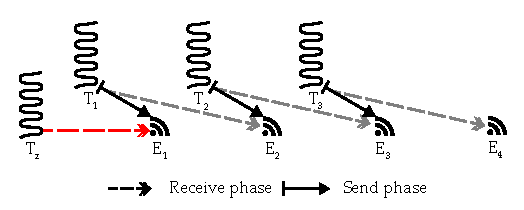
\includegraphics[width=\textwidth]{nbsendwait}
    \caption{The problem with \sendrecv.}
    \label{fig:send-wait}
\end{figure}

To illustrate the problem, we refer to \cref{fig:send-wait}, which shows four threads, $T_{z}$ and
$T_{1},T_{2},T_{3}$ and four endpoints, $E_{1},\dots,E_{4}$. Black arrows have already
occurred, blocking each thread on an endpoint, and grey are pending once each. $T_{1}$ has used \sendrecv on
$E_{1}$ and $E_{2}$, $T_{2}$ has used \sendrecv on $E_{2}$ and $E_{3}$,  
$T_{3}$ has used \sendrecv on $E_{3}$ and $E_{4}$. 
Because the send-phase is blocking, each thread $T_{n}$ is blocked waiting for the send to proceed 
on $E_{n}$. $T_{z}$ then uses \recv on $E_{1}$ (the red arrow), which triggers an unbounded chain of message
sending: $T_{1}$ finishes its send phase and begins the receive phase on $E_{2}$, which allows
$T_{2}$ to finish its send phase and being the receive phase on $E_{3}$, which allows $T_{3}$ to
finish its send phase and start the receive phase on $E_{4}$. This chain reaction is an
unbounded, long-running operation. By making the send-phase non-blocking such a chain reaction is not
possible: the send-phase is aborted as the endpoint has no threads waiting for a message on it, and
the receive phase then proceeds. 

\subsubsection{Yield}

% Maybe mention that additional yield functionality is provided in the sc invocation api with yieldto?
In baseline \selfour, \yield triggers a reschedule, and appends the calling thread to the end of the
appropriate scheduling queue. We retain these semantics for full scheduling contexts, however 
for partial, sporadic scheduling contexts \yield depletes the head sporadic replenishment immediately. The
caller is then blocked until the next replenishment becomes available, and then placed at the end of
the appropriate scheduling queue.

\begin{table}[t]
    \centering
    \rowcolors{2}{gray!25}{}
    \begin{tabularx}{\textwidth}{lXlll}\toprule
        \emph{System Call} & \emph{Class}       & \emph{Donation?} & \emph{New?} & \emph{Definition} \\\midrule
        \call              & sending, receiving & \yes             & \no         & \cref{api:call}\\
        \send              & sending            & \no              & \no         & \cref{api:send} \\
        \nbsend            & sending            & \no              & \no         & \cref{api:nbsend} \\
        \recv              & receiving          & \yes             & \no         & \cref{api:recv} \\
        \nbrecv            & receiving          & \yes             & \no         & \cref{api:nbrecv} \\
        \wait              & waiting            & \no              & \yes        & \cref{api:wait}\\
        \nbwait            & waiting            & \no              & \yes        & \cref{api:nbwait} \\
        \replyrecv         & sending, receiving & \yes             & \no         & \cref{api:replyrecv} \\
        \nbsendrecv        & sending, receiving & \yes             & \yes        & \cref{api:nbsendrecv} \\
        \nbsendwait        & sending, waiting   & \no              & \yes        & \cref{api:nbsendwait} \\
        \yield             & scheduling         & \no              & \no         & \cref{api:yield} \\
        \sout{\reply}      & \sout{sending}     & -                & -           & Removed \\
    \end{tabularx}
    \caption[New seL4 system call summary.]{New \selfour system call summary, indicating which system calls can trigger donation.
    and/or receiving messages. }
    \label{t:new-system-calls}
\end{table}

\cref{t:new-system-calls} summarises the new MCS system call API, while more detailed 
descriptions of each system call can be found in \cref{appendix:api}.

\subsection{Invocations}

Scheduling contexts have five invocations, listed in \cref{tab:sched_context_api}. Three of those
invocations are for binding \glspl{SCO} to \gls{TCB} and notification objects, while \scyieldto and 
\scconsumed facilitate user-level scheduling, allowing the user to manipulate
the kernel scheduling queues and to query the amount of time consumed by a specific \gls{SCO}.
Both functions return the amount of CPU time the scheduling context has consumed since it was last
cleared: reading the consumed value by either system call clears it, as does a timeout
exception.

The new control
capability, \schedcontrol, has only one invocation, \schedcontrolconfigure, for setting the parameters of a
scheduling context (the function definition can be found in \cref{api:schedcontrol_configure}). 
    
\begin{table}
    \centering
    \rowcolors{2}{gray!25}{}
    \begin{tabularx}{\textwidth}{lXl} \toprule
        \emph{Invocation} & \emph{Description} & \emph{Definition} \\\midrule
        \scbind    & Bind an object (TCB or Notification) to a \gls{SCO}. & \cref{api:schedcontext_bind} \\
        \scunbind  & Unbind all objects from a \gls{SCO}. & \cref{api:schedcontext_unbind} \\
        \scunbindobject & Unbind a specific object from a \gls{SCO}. & \cref{api:schedcontext_unbind_object}\\
        \scconsumed & Return the amount of time since the last timeout fault, \scconsumed or
        \scyieldto was called. & \cref{api:schedcontext_consumed}\\ 
        \scyieldto  & Place the thread bound to this \gls{SCO} at the front of its priority queue and return
        any time consumed. & \cref{api:schedcontext_yieldto}\\
        \bottomrule
    \end{tabularx}
    \caption{Scheduling context capability invocations.}
    \label{tab:sched_context_api}
\end{table}

As baseline \selfour only supports sending three capabilities in a single message (including to the
kernel), we add a second method for configuring multiple fields on a TCB in one system call
(\tcbsetschedparams), in addition to the existing method (\tcbconfigure). We avoid altering the
existing limit to avoid extensive re-verification of a non-critical path. Full configuration
of a TCB requires up to six capabilities to be set, not including timeout handlers, which are not
included in a combined configuration call as this is a less common operation. 
In total, we alter two invocations on TCB objects
and add three new invocations, shown in \cref{tab:tcb_api}. 

\begin{table}
    \centering
    \rowcolors{2}{gray!25}{}
    \begin{tabularx}{\textwidth}{lXll} \toprule
        \emph{Invocation} & \emph{Description} & \emph{New?} & \emph{Definition} \\\midrule
        \tcbconfigure & Set the cnode, vspace, and \gls{IPC} buffer. & \no & \cref{api:tcb_configure}\\
        \tcbsetmcpriority & Set the \gls{MCP}. & \yes & \cref{api:tcb_setmcpriority} \\
        \tcbsetpriority & Set the priority. & \no & \cref{api:tcb_setpriority} \\
        \tcbsetschedparams & Set \gls{SCO}, \gls{MCP}, priority and fault endpoint. & \yes &
        \cref{api:tcb_setschedparams} \\
        \tcbsettimeoutep & Set the timeout endpoint. & \yes & \cref{api:tcb_settimeoutep} \\
        \sout{\tcbsetaffinity}                 & Removed, now derived from \gls{SCO}.  & \no & N/A \\
        \bottomrule
    \end{tabularx}
    \caption{New and altered \gls{TCB} capability invocations.}
    \label{tab:tcb_api}
\end{table}

Finally, we remove the \cnodesavecaller invocation, which was previously used to move a reply
capability from the \gls{TCB} \cnode to a slot in the \gls{TCB} \cspace, and is no longer required
as the resume object capability is now provided to the receiving system call. 

\subsection{Scheduling context donation}

Conceptually there are three types of scheduling context donation: lending, returning, and
forwarding a scheduling context. The type of donation that occurs, and if it can occur, depends on
the system call used. 

Lending a scheduling context occurs between caller and callee on a \call, and
the semantics are simple: if a thread 
blocked on an endpoint does not have a scheduling context, the scheduling context is transferred
from sender (caller) to receiver (the callee), and the resume object is pushed
onto the call-stack, such that the \gls{SCO} can be returned. If the callee already has a scheduling
context, scheduling context donation does not occur. Note that lending also works for
handling faults, so thread fault handlers can be passive. Unlike previous versions of timeslice
donation in L4 kernels, there is no explicit flag for permitting donation: if the callee does not
have a scheduling context, the caller would block indefinitely, as the callee has no other way to
access processing time. As discussed in \cref{s:locking},
the caller in an RPC-style operation must trust the callee: regardless of the scheduling context
being executed upon, the callee can always choose to not reply, blocking the caller indefinitely. 

Lent scheduling contexts are returned when the resume object is invoked, or the head resume object
is deleted. Resume objects 
can be invoked directly by the send phase of a system call, or indirectly, by using the
resume object in the receive phase of a system call, thereby clearing it for another client to block
on, or deleting the resume object.
Regardless of the state of the callee, the \gls{SCO} is returned, which if done
incorrectly (via a \send), can leave the callee not blocked on an endpoint, and consequently 
unable to receive further scheduling contexts via donation or lending. Correct usage by a passive thread is with \replyrecv,
\nbsendrecv, blocking the passive thread such that it is ready to receive another scheduling
context. Like lending, scheduling contexts can also be returned by a fault handler replying to a fault message.

Forwarding a scheduling context does not establish a call-chain relationship, and allows
for scheduling contexts to be transferred between threads in non-RPC patterns. The semantics are
as follows: if \gls{IPC} forwarding is used via \nbsendrecv (\cref{s:ipc-forwarding}) is used, and the receiver does not have a scheduling context,
the scheduling context is forwarded. 

Scheduling contexts can only be donated and received on specific system calls, indicated in
\cref{t:new-system-calls}. 

\subsubsection{Passive servers}
\label{sec:impl-passive-servers}

Passive servers do not have scheduling contexts, yet they must be waiting on an endpoint in order to
receive \glspl{SCO} over \gls{IPC}, and possibly initialise some server-specific state first.
The protocol for initialising passive servers is to start them as
active, then wait for the server to signal to the initialising thread that they are ready to be
converted to passive. IPC forwarding can be used to do this, so the passive server can send a
message on one endpoint or notification object, then wait on another to receive \glspl{SCO} over
IPC. Example user-level code for this process is 
provided in \cref{list:passive-server}. 

\begin{listing}[t]
\begin{minted}{c}
void initialiser(seL4_CPtr server_tcb, seL4_CPtr init_sc, seL4_CPtr init_endpoint) {
  /* start server */
  seL4_TCB_Resume(server_tcb);
  /* wait for the server to tell us it is initialised */
  seL4_Wait(init_endpoint, NULL);
  /* convert the server to passive */
  seL4_SchedContext_Unbind(init_sc);
}

void passive_server(seL4_CPtr init_endpoint, seL4_CPtr endpoint, seL4_CPtr reply) {  
  seL4_MessageInfo_t info = init_server_state();
  seL4_Word badge;

  /* signal to the initialiser that this server is ready to be converted to passive, and block on the endpoint with resume object reply */
  info = seL4_NBSendRecv(init_endpoint, info, endpoint, &badge, reply);
  while (true) {
    /* when the server wakes, it is running on a client scheduling context */
    info = process_request(sender);
    /* reply to the client and block on endpoint, with resume object reply */
    seL4_ReplyRecv(endpoint, info, &badge, reply);
  }
}

void client(seL4_CPtr endpoint, seL4_MessageInfo_t message) {
  /* send a message to the passive server */
  seL4_Call(endpoint, message);
}
\end{minted}
\caption{Example initialiser, passive server, and client.}
\label{list:passive-server}
\end{listing}

\subsubsection{Notification Binding}

Passive servers can receive scheduling contexts from their bound notification object, allowing for
the construction of single-threaded servers which receive both notifications and IPC messages. 
The semantics are as follows: if a TCB receives a notification from its bound notification
object, and that TCB does not have a scheduling context, the TCB receives the scheduling context.
If a TCB blocks on an endpoint, and is running on its bound notification object, the TCB is
rendered passive again. 

\section{Data Structures and Algorithms}

Now we discuss changes to the data structures and algorithms added and changed in the kernel to provide
accounting, which charges CPU time to the correct \gls{SCO}, and the enforcement mechanisms, which requires
a new scheduling data structure and fault type.

\subsection{Accounting}

All processing time is accounted to the scheduling context of the currently running \gls{TCB}. 
In this section we first establish \emph{how} that time is accounted, and then \emph{when} it is
accounted.

There are two ways to account for time in an \gls{OS} kernel:
\begin{itemize}
    \item in fixed time quanta, referred to as \emph{ticks},
    \item in actual time passed between events, referred to as \emph{tickless}.
\end{itemize}

Using ticks, timer interrupts are set for a periodic tick and are
handled even if no kernel operation is required, incurring a preemption overhead.
This approach has the advantage of simplicity: the timer implementation in the kernel is 
stateless and the timer driver can be set once, periodically, never requiring reprogramming. 
In older-generation hardware, especially x86, reprogramming the timer device incurred a 
significant cost, enough to ameliorate the preemption overhead. 
However, this design is not without limitations:
the precision of the scheduler is reduced to the length of the tick. Precision must be traded for
preemption overhead: reducing the tick length increases precision, but also increases 
preemption overhead. Preemption overhead is particularly problematic for real-time systems, as
the \gls{WCET} each real-time task is inflated by the \gls{WCET} of the kernel for every preemption.

Tickless kernels remove this trade-off by setting timer interrupts for the exact time of the next
event. As we will show in \cref{s:eval-timer}, the cost of reprogramming the timer device on modern
hardware is smaller, rendering the tickless design feasible. Consequently, we convert \selfour
to a tickless kernel, a non-trivial change due to the fact that the kernel is
non-preemptible\footnote{Save for
explicit preemption points in a few long-running operations.}, which means timer interrupts for the
scheduler can only be serviced when the kernel is not running. Allowing a thread to complete an
operation in the kernel when it does not have sufficient time to do so would violate temporal
isolation, as the bandwidth allocated to the scheduling context could then be exceeded. As a result,  
on kernel entry, the calling thread must have sufficient budget to complete the operation. Without
further decoding a pending system call, the kernel cannot tell which operation a thread is
attempting, so sufficient budget becomes the \gls{WCET} of the kernel.

Threads are not permitted in the scheduler if they have insufficient budget, as if the scheduling
algorithm must iterate until a thread with sufficient budget is discovered, the complexity of the
algorithm becomes $O(n)$ in the number of threads. The same condition holds for IPC endpoint queues:
we take the time on kernel entry in order to charge a preempting thread, and any time from kernel
entry is accounted to the scheduling context active at kernel exit. Because a passive scheduling context
then must be able to be charged not only for the entry path into the kernel, but the exit path, the
sufficient budget is actually \emph{twice} the \gls{WCET} of the kernel.

We check budget sufficiency on kernel entry, by reading the current timestamp and storing 
the amount of time consumed since the last kernel entry, allowing us to detect budget expiry in a single 
point, and carry on other kernel operations with this assumption intact. This means that timeout 
faults can only be raised at once point in the kernel, greatly simplifying the implementation by
avoiding excessive checks in other paths. 

\begin{figure}
    \centering 
    \includegraphics[width=0.7\textwidth]{tickless}
    \caption{New tickless kernel structure.}
    \label{figure:tickless}
\end{figure}


\subsubsection{Fastpath}
\label{p:impl-fastpath}

We alter the IPC fastpath conditions introduced in \cref{sec:sel4-fastpath} to include one
more condition to have a very low overhead on fastpath performance:
\begin{itemize}
    \item The receiver must be passive. For \call, this means the callee must be passive, and
          for \replyrecv, the TCB blocked on the resume object must be passive.
\end{itemize}
This is because
although timer device access is cheaper on modern hardware, it is not free. It also allows us to
avoid checking budgets and modifying sporadic replenishments on the fastpath, operations which have
many conditional branches, which would also increase overheads. Note that we expect most servers in
real systems to use passive servers for \gls{RPC}, even for non real-time systems, to assure
fairness of resource access between round-robin threads.  

Even on the slowpath, we avoid reprogramming the timer unless it is required. Like reading the time, 
reprogramming the timer is cheaper, but not free. Consequently although we update the current time
on every entry, we only charge threads at specific points:
\begin{itemize}
\item when the timer interrupt has fired, so clearly the timer needs reprogramming,
\item when the current scheduling context changes, so a different interrupt is required,
\item when the kernel timestamp has been acted upon: for instance, the used to schedule a
    replenishment.
\end{itemize}
If the recorded timestamp is not acted upon, the time is rolled back to the previously recorded value,
thus avoiding reprogramming the timer unnecessarily.

\cref{figure:tickless} illustrates the new control flow of the tickless kernel, and shows
how and when processing time is charged to scheduling contexts.
On kernel entry, if the available budget is insufficient, the kernel pretends the timer has already fired,
resets the budget and adds the thread to the release queue. If the entry was due to a system call,
the thread will retry that call once it wakes with further budget.
Once the thread is awoken, it will retry the system call.

\subsubsection{Domain scheduler}

We retain the domain scheduler which, as discussed in \cref{sec:sel4-domain-scheduler}, is required
for the proof of confidentiality~\citep{Murray_MBGBSLGK_13}. However, we convert the 
implementation to tickless, such that domains are
configured with CPU cycles to execute, rather than fixed ticks, which no longer exist.

\subsection{Enforcement}

% timeout exceptions, release queue, sporadic servers
The enforcement mechanisms require the most significant changes to the kernel, which we now detail.
The main change required to the existing scheduler is the addition of a \emph{release queue} per
processing core which contains all runnable threads waiting for a replenishment. If a
preempted thread does not have any available replenishments, the kernel removes the thread from the
ready queue.

\subsubsection{Priority queues}

In addition to the release queue, we also change endpoint- and notification-object queues
to priority queues, ordered by \gls{TCB} priority. All queues are implemented as ordered, doubly-linked
lists, where all operations complete in $O(1)$ except for insertion, which is $O(n)$, where $n$ 
is the number of threads in the queue. 
We chose the list data structure over a heap for increased performance and reduced verification
burden.

A list-based priority queue out-performs a heap-based priority queue for small $n$ (in our
implementation up to around $n = 100$).  This $n$ is larger than one would expect in a traditional
\gls{OS}, where heap implementations are array-based in contiguous memory with layouts optimised for
cache usage.  However, because \selfour kernel memory is
managed at user-level (as discussed in \cref{sec:sel4-memory}), data structures must be dynamic, 
resulting in much higher code complexity, and poorer performance than a static heap. 
For endpoint queues, it is reasonable to expect low amounts of threads, as many threads queuing on
an endpoint at once indicates a poor system design. For the release queue, the restriction
becomes a function of the user-level admission test: only scheduling contexts with 
partial budgets are placed into the release queue, which limits the size of the queue.
Consequently we do not expect any of the priority queues to contain large amounts of tasks,
however if scalability becomes a problem in
practice this implementation could be reconsidered. \citet{Brandenburg:phd} used
binomial heaps for schedulers in \litmus, however Linux does not provide the guarantees, or
implementation requirements of \selfour.

One security concern is sub-systems with access to a single scheduling context and a large amount
of memory can increase the kernel's run-time by queuing up a large amount of passive threads on 
an endpoint. To prevent this, system designers must not hand out large untyped capabilities to
untrusted sub-systems. 

\subsubsection{Timeout Exception Handlers}

Timeout exceptions are only triggered for threads with non-empty timeout handling slots in the
\gls{TCB} \cnode, configured with \tcbsettimeoutep. The implementation is the same as for
fault handlers, with one exception: while fault \gls{IPC} messages can trigger scheduling context
donation, allowing fault-handling threads to be passive, timeout messages cannot. The timeout
message contains the badge of the scheduling context which triggered the fault, and the amount of
time consumed by that scheduling context since the last reset.

\section{Summary}

In this chapter we have presented the new kernel objects, system call API, invocations and 
structural changes made to provide mechanisms for temporal isolation. 
The implementation adds roughly 2,000 lines of code to \selfour (14\% increase), as measured
by source lines of code (SLOC)~\citep{Wheeler_01} on the pre-processed code for the \textsc{Sabre}, the verified platform.
In the next chapter, we evaluate our implementation with a series of microbenchmarks, 
system benchmarks and case studies.



\chapter{Evaluation}
\label{chap:evaluation}

We now evaluate our model through a series of microbenchmarks, system benchmarks and case studies.
First, we present the ARM and x86 hardware platforms used in addition to the cost of timer operations on those
platforms. Then we demonstrate the low performance overhead of our mechanisms using a set of 
microbenchmarks that measure the overheads of the MCS kernel versus a baseline. The baseline kernel
is \selfour, at development version 7.0.0 with some added experimental fastpaths for interrupt and signal
handling. Both kernels are branches of \selfour with the same merge-base, \ie both branches divert from the master branch at
the same point. The exact revisions used are available online at:
\begin{description}
    \item[Baseline:] \url{https://github.com/pingerino/seL4/releases/tag/phd-baseline},
    \item[MCS:] \url{https://github.com/pingerino/seL4/releases/tag/phd-MCS}.
\end{description}

We then run several system benchmarks, first comparing a Redis~\citep{redis:url} 
implementation to baseline \selfour, Linux and NetBSD to show that our kernel is competitive.
We then demonstrate temporal
isolation between threads sharing the same CPU in two scenarios,
using Redis again, followed by \code{ipbench}~\citep{Wienand_Macpherson_04}. We then show isolation in a
shared encryption server, and measure the cost of various timeout fault-handling policies. 

In addition, we evaluate two user-level scheduler implementations: one which implements a static
criticality switch, and a user-level \gls{EDF} implementation which we show is
competitive with an in-kernel \gls{EDF} scheduling from \litmus. Lastly, we use an \gls{IPC}
throughput benchmark to demonstrate low multicore-scalability overhead, and we show 
how resource server threads can migrate between processing cores.

\section{Hardware}

% describe benchmark setup, details of each hardware platform
We run microbenchmarks on a variety of hardware to show the overheads of the model compared to
baseline \selfour. \Cref{t:evaluation-hardware} summarises the hardware platforms. \textsc{Sabre} is
the verified platform for \selfour and, at the time of writing, verification of the \text{x64}
platform is in progress.
Currently, the only platforms with support for more than one core in \selfour are \textsc{Sabre},
and \textsc{x64}.

Our ARM development boards for each \gls{SoC} are as follows:
\begin{itemize}
    \item \textsc{KZM}: NXP i.MX31 Lite development kit.
    \item \textsc{Sabre}: NXP Sabre Lite development board.
    \item \textsc{HiKey}: LeMaker HiKey. 
    \item \textsc{TX1}: NVIDIA Jetson TX1 development kit.
\end{itemize}

Two of our platforms, \textsc{x64} and \textsc{HiKey} support both 32- and 64-bit execution modes.
We use both, referring to them as \textsc{ia32} and \textsc{HiKey32} when in 32-bit mode and
\textsc{x64} and \textsc{HiKey64} otherwise. All platforms have out-of-order execution, except
\textsc{HiKey}, which is in-order, and \textsc{KZM}, which has in-order execution and out-of-order
from some operations (\eg stores). \textsc{TX1} currently only has 64-bit support on \selfour.

Additionally, we use several load generators running Linux on an isolated network for 
benchmarks that require a network.

\begin{table}[t]
\begin{tabularx}{\textwidth}{Xlrrrrr}\toprule
    \emph{Platform}       & \emph{CPU} & \emph{Clock } & L1 & L2 & L3  & TLB  \\
    \emph{Arch}           & \emph{SoC/Family}        & GHz           & (KiB) & (KiB) & (MiB) & (entries) \\\midrule
    \textbf{\textsc{KZM}} (32-bit) & ARM1136JF-S       & 1.0           & 16+16       & 128      & \no      & 32\\
    \small{ARMv6}                 & NXP i.MX31            &               & 4$\times$        & 8$\times$         & \no      & 2$\times$  \\
    \rowcolor{gray!25}
    \textbf{\textsc{Sabre}} (32-bit) & Cortex-A9       & 1.0           & 32+32    & 1024     & \no      & 64\\
    \rowcolor{gray!25}
    \small{ARMv7}                    & NXP i.MX6             &               & 4$\times$  & 16 $\times$  & \no & 2$\times$  \\
    \textbf{\textsc{HiKey}} (64-bit)  & Cortex-A53        & 1.2           & 32+32     & 512 & \no & 128         \\
    \small{ARMv8}                    & Kirin 620         &               & 4$\times$+2$\times$       & 16$\times$    & \no   & 4$\times$  \\
    \rowcolor{gray!25}
    \textbf{\textsc{TX1}}   (64-bit)  & Cortex-A57        & 1.9           &  32+48 & 2,048 & \no & 256          \\
    \rowcolor{gray!25}
    \small{ARMv8}                   & Jetson TX1  &                   & 2$\times$+3$\times$       & 16$\times$ & \no & 4$\times$ \\
    \textbf{\textsc{x64}}    (64-bit) & i7-4770           & 3.1           & 32+32 & 256 & 8 & 128,8 \\          
    \small{x86}                     & Haswell            &                 & 8$\times$ & 8$\times$ & 16$\times$ & 8$\times$ \\
    \bottomrule
\end{tabularx}
\caption[Hardware platform details.]{Hardware platform details, ``$\times$`` is associativity, and + indicates I-cache+D-cache.}
\label{t:evaluation-hardware}
\end{table}

\section{Overheads}

We first present a suite of microbenchmarks to evaluate any performance overheads against baseline
\selfour.
Because the kernel uses \emph{lazy switching} for the \gls{FPU}, meaning that the \gls{FPU} context is only
switched if it is actively being used, we ensure that \gls{FPU} context switching
is off. This is achieved by performing the required number of system calls 
without activating the \gls{FPU}. We present
overheads on IPC operations, signalling and interrupts, and finally scheduling. 

For each of the benchmarks in this section, we measure the cost of measurement, which is the cost of reading the
cycle counter on ARM platforms, and the \gls{TSC} on x86, and subtract the value obtained
from the final result.

\subsection{Timer}
\label{s:eval-timer}

Two of the main sources of overhead introduced by our model are related to the need to read and
reprogram the timer on non-fastpath kernel entries, and when performing a scheduling context switch.
We show the results of microbenchmarks of both of these operations in \Cref{t:evaluation-timer}, and
note the timer hardware used on the specific platform. 

\begin{table}[t]\centering
\rowcolors{2}{gray!25}{white}
\begin{tabularx}{\textwidth}{lXccc}\toprule
    \emph{Platform} & \emph{Timer} & \emph{Read time} & \emph{Set timeout} & \emph{Sum}
    \\\midrule
    \textsc{KZM}               & General purpose timer    & 83 (0)   & 203(0)  & 286   \\
    \textsc{Sabre}             & ARM MPCore global timer  & 23 (0)   & 36 (0)  & 59    \\
    \textsc{HiKey32/64}        & ARM generic timers       &  6 (0)   &  6 (0)  & 12    \\
    \textsc{TX1}               & ARM generic timers       &  8 (0)   &  1 (0)  & 9     \\
    \textsc{ia32}              & TSC deadline mode        & 12 (2.2) & 220 (1.0) & 232 \\
    \textsc{x64}               & TSC deadline mode        & 11 (2.3) & 217 (2.0) & 228 \\
    \bottomrule\hline
\end{tabularx}
\caption[Latency of timer operations.]{Latency of timer operations per platform in cycles. Standard deviations shown
in parentheses.}
\label{t:evaluation-timer}
\end{table}

For both microbenchmarks, we read the timestamp before and after the operation, and do this 102
times, discarding the first two results to prime the cache.  We take the difference of the cycle
counts, and subtract the cost of measuring the cycle counter itself. The results show the cost of
both operations separately, and then their sum, which is the total measured overhead introduced by timers on
scheduling context switch.

All platforms excluding \textsc{KZM} have a 64-bit timer available, making \textsc{KZM} the only
platform requiring timer overflow interrupts. These are not measured as \textsc{KZM} is a deprecated
platform provided for comparison with modern ARM versions.

\textsc{KZM} and \textsc{Sabre} both use memory-mapped timers, the 32-bit general purpose timer for
the former and 64-bit ARM global timer for the latter. \textsc{Sabre} has four cores and while the
timer device is shared, the timer registers are per-core, making access fast. 
Timer access on \textsc{Sabre} is significantly faster than the \textsc{KZM}. 

For all other ARM platforms, the ARM generic timers are available, which are accessed via the
coprocessor. The majority of new ARM platforms support the ARM generic timers. 

On \textsc{x64} we use the \gls{TSC} with \gls{TSC}-deadline
mode~\citep{Intel_64_IA-32:asdmspg_325384}, an architectural \gls{MSR} available since
Intel SandyBridge. A local-APIC timer interrupt is triggered when the \gls{TSC} matches the
value written to the \gls{MSR}. 
In practice, especially
for \textsc{x64}, timer operations are subject to pipeline parallelism and out-of-order execution, which
reduces the overhead.

Results on both architectures show that the overhead of a tickless kernel, which requires the timers
to be frequently read and reprogrammed, is tolerable on modern hardware. On ARM, timer costs have
reduced by an order of magnitude from ARMv6 through to ARMv8. 
\clearpage
\subsection{IPC performance}

\Gls{IPC} performance is a critical measure of the practicality and efficiency of a
microkernel~\citep{Liedtke_95}. We benchmark our \gls{IPC} operations against baseline \selfour,
which has an established efficient \gls{IPC} fastpath~\citep{Elphinstone_Heiser_13}. 

\subsubsection{Fastpath}

To evaluate IPC fastpath performance, we set up a client (the caller) and server (the callee) in different
address spaces. We take timestamps on either side of the IPC operation being benchmarked and record
the difference. This is done 16 times for each result value to prime the cache, then record the next
value. Results presented are for performing this a total of 16 times. Additionally, we measure the
overhead of system call stubs in the same way and subtract this from the measurement, to obtain
only the kernel cost of the operation\footnote{The \gls{IPC} benchmarks already existed for
 \selfour, but we modify them to support the \gls{MCS} kernel as part of this thesis.}.
   The message sent is zero length, so neither the caller nor callee's \gls{IPC} buffer is accessed.

As discussed in \cref{p:impl-fastpath}, timer operations are avoided on the fastpath. However, we do
add significantly to the \call fastpath, by accessing two further objects (the scheduling context
and resume object) and two validation checks. In detail, the \call fastpath is altered as follows:

\begin{table}[t]\centering
    \rowcolors{2}{gray!25}{white}
    \begin{tabularx}{\textwidth}{Xrrrrrr}\toprule
        \emph{Platform}     
                                & \multicolumn{2}{c}{\emph{Baseline}}
                                & \multicolumn{2}{c}{\emph{MCS     }}
                                & \multicolumn{2}{c}{\emph{Overhead}} \\\midrule
    \ipcmicro{KZM}{kzm}{call-fastpath}
    \ipcmicro{Sabre}{sabre}{call-fastpath}
    \ipcmicro{HiKey32}{hikey32}{call-fastpath}
    \ipcmicro{HiKey64}{hikey64}{call-fastpath}
    \ipcmicro{TX1}{tx1}{call-fastpath}
    \ipcmicro{ia32}{ia32}{call-fastpath}
    \ipcmicro{x64}{haswell}{call-fastpath}
    \bottomrule
\end{tabularx}
\caption[Fastpath IPC overhead (\call)]{Time in cycles for the \call fastpath. Standard deviations shown in parentheses.}
\label{t:fastpath-ipc-micro-call}
\end{table}
\begin{table}[t]\centering
    \rowcolors{2}{gray!25}{white}
    \begin{tabularx}{\textwidth}{Xrrrrrr}\toprule
        \emph{Platform}      
                                & \multicolumn{2}{c}{\emph{Baseline}}
                                & \multicolumn{2}{c}{\emph{MCS     }}
                                & \multicolumn{2}{c}{\emph{Overhead}} \\\midrule
 
    \ipcmicro{KZM}{kzm}{reply-fastpath}
    \ipcmicro{Sabre}{sabre}{reply-fastpath}
    \ipcmicro{HiKey32}{hikey32}{reply-fastpath}
    \ipcmicro{HiKey64}{hikey64}{reply-fastpath}
    \ipcmicro{TX1}{tx1}{reply-fastpath}
    \ipcmicro{ia32}{ia32}{reply-fastpath}
    \ipcmicro{x64}{haswell}{reply-fastpath}
    \bottomrule
\end{tabularx}
\caption[Fastpath IPC overhead (\replyrecv)]{Time in cycles for the \replyrecv fastpath. Standard deviations shown in parentheses.}
\label{t:fastpath-ipc-micro-reply}
\end{table}

\begin{itemize}
\item We remove the reply capability lookup, so the sending \gls{TCB}'s \cnode is no
        longer accessed. 
\item We read the resume object pointer from the thread state, however the thread state is already accessed
    by the \call fastpath. 
\item We check that the resume object is valid. 
\item We read from and write to the resume object to push it onto the call stack.
\item We check the destination \gls{TCB} is passive.
\item We write scheduling context that is lent over the \call to link it to the receiver, and update
    the back pointer to the resume object.
\end{itemize}


\cref{t:fastpath-ipc-micro-call} shows the results.
Overheads on the \call fastpath are low, with the worst affected platform being
\textsc{KZM} with a 10\% overhead, which is the oldest platform with the smallest caches. On call,
\textsc{KZM} shows L1 data cache miss and 1 memory access, which is likely an unlucky
cache-conflict. \textsc{Sabre} suffers a 28\% overhead with high variance, due to a \gls{TLB} miss likely
due to the relatively low associativity on Cortex-A9 \glspl{TLB}.  In general, as hardware becomes newer the
overhead is lower, with the exception of the \textsc{HiKey}, which is the only platform we use that has 
in-order execution. Additionally \textsc{HiKey} has a smaller L2 cache than the older \textsc{Sabre},
but a larger \gls{TLB} with higher associativity.
We posit that for the HiKey, further hand optimisation of the fastpath would result in better
performance. The newest ARM hardware is the TX1, which only shows a 5\% overhead. x86 with its large
caches and highly optimised pipeline only incurs a 1\% overhead. For further detail on the
numbers read from the performance counters cited here, please see
\cref{appendix:fastpath-performance}. On \textsc{ia32} we see a minor reduction in the time for
\call, although the instructions executed increases: this is most likely due to the long pipeline,
and increased instructions reducing data dependencies. Overall for x86 fastpath overheads are low. 

The fastpath for \replyrecv has a higher impact, for two reasons: first, we add a new capability
lookup, being the resume object provided to receive, which must be looked up by the \replyrecv
fastpath. Although we remove the reply capability from the \gls{TCB}
\cnode, that \cnode is still accessed to validate the caller's root \cnode capability
and top-level page directory capability, so the cache-foot print is not reduced. Additionally, because
\gls{IPC} is now priority ordered, the fastpath must check if the callee's \gls{TCB} will be appended to the
endpoint queue. Otherwise, the fastpath is aborted for an ordered insert. 

As a result, the overheads shown in \cref{t:fastpath-ipc-micro-reply} for \replyrecv are generally higher
than \call, except for \textsc{Sabre}, which already suffered some \gls{TLB} misses on
the baseline kernel, again due to low \gls{TLB} associativity.
\clearpage

\subsubsection{Slowpath}
\label{eval:slowpath}

\begin{table}[t]\centering
    \rowcolors{2}{gray!25}{white}
    \begin{tabularx}{\textwidth}{Xlllllll}\toprule
        \input{data/generated/avg_slowpath_round_trip_passive.inc}
        \bottomrule
    \end{tabularx}
    \caption{Passive slowpath round-trip IPC overhead.}
    \label{t:slowpath-ipc-micro}
\end{table}
Now we evaluate the \gls{IPC} slowpath, for both active and passive threads in the same address
space.
Unlike the fastpath, the slowpath
generally does not fit into the cache. Consequently, precise measurements like those done for the
fastpath show erratic results with high standard deviations on our hardware. Instead, we run average
benchmarks for the slowpath, where for 110 runs, we measure the time taken for 10,000 IPC pairs
(\call, \replyrecv) and divide by 10,000 to get a result, abandoning the first 10 results. 
In order to hit the slowpath we make the message length 10 words, which exceeds
the fastpath condition that the message should fit into registers.

We run the benchmark for both active and passive threads, which shows the overhead of changing a
scheduling context versus not. \cref{t:slowpath-ipc-micro} shows the results for the passive
slowpath and \cref{t:slowpath-ipc-micro-active} for active, where the top row in the table is 
the baseline number, the second row is the overhead when
comparing the number of cycles taken for the benchmark. Every other row shows the difference in value of the 
listed performance counter between baseline and MCS. We do not show standard deviations, however
they are measured and are very small (either 0 or a few percent of the mean). 

Passive slowpath overhead, as shown in \cref{t:slowpath-ipc-micro} is not small;
this is due to the fact that the seL4 scheduler has far more
functionality than previously, increasing the code size, and the cache foot print is higher, given
that the resume object and scheduling context must be accessed in addition to the \glspl{TCB} of the
caller and callee. Looking at ARM platforms, the overhead reduces drastically as hardware becomes
more modern: for the most part, this means that the caches are bigger, and timer access costs are
smaller. Except for the \textsc{HiKey} platform, with has an in-order
execution pipeline and a smaller L2 cache than the \textsc{Sabre}. We suspect that the overheads could be reduced on HiKey with more careful hand
optimisation. 64-bit HiKey has nearly half the excess instructions when compared to 32-bit, and 
50\% less memory accesses, resulting in far less overhead on \textsc{HiKey64} than \textsc{HiKey32}.
\textsc{Sabre} suffers from the low-associativity of its \gls{TLB} with misses in both the instruction and
data TLBs. On the x86 platform, both \textsc{ia32} and \textsc{x64} show the same overhead in terms
of ratio, both due to the increase in instructions.

Another factor that complicates the slowpath is the compiler. We use GCC version 5.5.0 with optimisation
level O2 for all benchmarks, with the \code{mtune} parameter set as appropriate. All kernel
code is pre-processed and concatenated into to single file with the \code{whole-program} attribute
set which allows for greater compiler optimisations. However, the level of optimisation for a
specific platform, especially ARM platforms, is not known and contributes to the variance between
platforms, and between arm versions.

Additionally, it should be noted that the slowpath is avoided in most cases, as long IPC is discouraged in
favour of establishing shared memory protocols to transfer large amounts of data. The majority of
fastpath checks make sure the thread being switched to is valid and runnable. Only two cases hit the
slowpath frequently: if a medium priority thread has woken, and is higher priority than the
\gls{IPC} target, and if the target is active, not passive. 
Additionally, many improvements can be made to the \gls{IPC} slowpath to improve
performance, but it has not been examined extensively.

\begin{table}[t]\centering
    \rowcolors{2}{gray!25}{white}
    \begin{tabularx}{\textwidth}{Xlllllll}\toprule
        \input{data/generated/avg_slowpath_round_trip.inc}
        \bottomrule
    \end{tabularx}
\caption{Active slowpath round-trip IPC overhead.}
\label{t:slowpath-ipc-micro-active}
\end{table}


\cref{t:slowpath-ipc-micro-active} shows results for the active slowpath, and has higher overheads
again. In this case, we change scheduling
contexts, so not only does another object (the second \gls{SCO}) need to be accessed, but the timer
needs to be reprogrammed, and sporadic replenishment logic applied. \textsc{TX1} and
\textsc{HiKey64} have the lowest overhead, although the overhead looks to be ameliorated by lucky
data placement with a reduction in L1 D-cache misses on both platforms. The vast majority of
overhead comes from timer access and reprogramming, far more instructions executed, and on platforms
with small caches or low-associativity, the increase in cache footprint.  


\subsection{Faults}

\begin{table}[t]\centering
    \rowcolors{2}{gray!25}{white}
    \begin{tabularx}{\textwidth}{Xllllll}\toprule
\input{data/generated/avg_fault_round_trip_passive.inc}
    \bottomrule
\end{tabularx}
\caption{Passive fault round-trip IPC overhead.}
\label{t:slowpath-fault-micro}
\end{table}

\begin{table}[b]\centering
    \rowcolors{2}{gray!25}{white}
    \begin{tabularx}{\textwidth}{Xllllll}\toprule
\input{data/generated/avg_fault_round_trip.inc}
    \bottomrule
\end{tabularx}
\caption{Active fault round-trip IPC overhead.}
\label{t:slowpath-fault-micro-passive}
\end{table}

Recall that fault handling in \selfour occurs via an \gls{IPC}, simulated by the kernel, to a fault
endpoint, which a fault handling-thread can wait upon for messages (\cref{api:faults}). 
To measure the fault-handling cost, we run two threads in the same address space: a fault handler
and a faulting thread, with the same priority. We trigger a fault by executing an undefined instruction in a loop on the faulting thread's
side. The fault handler then increments the instruction pointer past the undefined
instruction, and the benchmark continues.  As this is also a slowpath, we use the same method as
above, and measure the amount of time it takes for 10,000 faults then divide the result. We do this
for 110 runs, abandoning the first 10, to calculate the standard deviation and average. 

We measure both active and passive fault handling, and the results, shown in
\cref{t:slowpath-fault-micro}, are similar to slowpath
\gls{IPC}, being slower for active, and improving as cache-size and timer operation cost reduces. 
Note that although there is currently no fastpath for fault handling, it is merely a matter of
engineering effort to add one should this become a performance issue. 

We do not show results for the \textsc{KZM} platform, as it is ARMv6 and the performance monitor
unit, including the cycle counter, cannot be read from user mode. As a result we use the
undefined instruction to read the cycle counter efficiently on this platform, 
so the fault benchmark does not work.
\clearpage
\subsection{Experimental fastpaths}

As noted in the previous section, mainly engineering effort is required to add new fastpaths. For
this reason, we add two new (non-verified) experimental fastpaths to both kernels: one for interrupt
delivery, and the other for signalling a low-priority thread. We measure baseline versus MCS results
for both operations, with and without the fastpaths.

\subsubsection{Interrupt fastpath}

We measure interrupt latency using two threads, one spinning in a loop
updating a volatile cycle counter, the other, higher priority thread
waiting for an interrupt. On delivery, the handler thread determines the
interrupt latency by subtracting the
looped timestamp from the current time. We repeat this loop 110 times, discarding the first 10
results.

For the interrupt path, the experimental fastpath covers the case where either the interrupt
does not result in a context switch, or the interrupt results in a switch to a higher-priority
runnable thread. Note that this would be faster if we picked one of the cases, however without
workload specifics, it is not clear whether one of these operations should be prioritised over the
other. Additionally, as interrupts are by their nature preemptive, we must switch scheduling
contexts, which incurs the time to reprogram the timer and charge the previous thread. In both cases,
the scheduler itself is avoided. 


\begin{table}[t]\centering
    \rowcolors{2}{gray!25}{white}
    \begin{tabularx}{\textwidth}{Xrrrrrr}\toprule
        \emph{Platform (faspath?)}    
                                & \multicolumn{2}{c}{\emph{Baseline}}
                                & \multicolumn{2}{c}{\emph{MCS     }}
                                & \multicolumn{2}{c}{\emph{Overhead}} \\\midrule
        \irqmicro{KZM \yes}{kzm}
        \irqmicro{KZM \no}{kzm-nfp}
    \irqmicro{Sabre \yes}{sabre}
    \irqmicro{Sabre \no}{sabre-nfp}
    \irqmicro{HiKey32 \yes}{hikey32}
    \irqmicro{HiKey32 \no}{hikey32-nfp}
    \irqmicro{HiKey64 \yes}{hikey64}
    \irqmicro{HiKey64 \no}{hikey64-nfp}
    \irqmicro{TX1 \yes}{tx1}
    \irqmicro{TX1 \no}{tx1-nfp}
    \irqmicro{ia32 \yes}{ia32}
    \irqmicro{ia32 \no}{ia32-nfp}
    \irqmicro{x64 \yes}{haswell}
    \irqmicro{x64 \no}{haswell-nfp}
    \bottomrule
\end{tabularx}
\caption[Fastpath and non-fastpath IRQ overhead.]{Fastpath and non-fastpath IRQ overhead in cycles, baseline
    \selfour versus MCS. Standard deviations shown in parentheses.}
\label{t:micro-irq}
\end{table}

\cref{t:micro-irq} shows the results. On most platforms, the overhead remains the same regardless of
the fastpath or not, except on x86 platforms. In the case of the ARM platforms, the IRQ fastpath
yields a performance improvement of a few hundred cycles, which can ameliorate somewhat the
overheads of the MCS model, but not completely. In this case we see the majority of the MCS overhead
is due to the operations required to switch scheduling contexts. \textsc{KZM} shows the  highest overhead, where once again we
exceed the small cache. The \textsc{HiKey} pays for its in-order execution pipeline, which could be
improved with further profiling of the fastpath. The \textsc{TX1} shows the least impact, with only
a 6\% increase on the interrupt fastpath. 
%\clearpage

\subsubsection{Signal}

\begin{table}[b]\centering
    \rowcolors{2}{gray!25}{white}
    \begin{tabularx}{\textwidth}{Xrrrrrr}\toprule
        \emph{Platform (fastpath?)}     
                                & \multicolumn{2}{c}{\emph{Baseline}}
                                & \multicolumn{2}{c}{\emph{MCS     }}
                                & \multicolumn{2}{c}{\emph{Overhead}} \\\midrule
    \sigmicro{KZM \yes}{kzm}
    \sigmicro{KZM \no}{kzm-nfp}
    \sigmicro{Sabre \yes}{sabre}
    \sigmicro{Sabre \no}{sabre-nfp}
    \sigmicro{HiKey32 \yes}{hikey32}
    \sigmicro{HiKey32 \no}{hikey32-nfp}
    \sigmicro{HiKey64 \yes}{hikey64}
    \sigmicro{HiKey64 \no}{hikey64-nfp}
\sigmicro{TX1 \yes}{tx1}
\sigmicro{TX1 \no}{tx1-nfp}
    \sigmicro{ia32 \yes}{ia32}
    \sigmicro{ia32 \no}{ia32-nfp}
    \sigmicro{x64 \yes}{haswell}
    \sigmicro{x64 \no}{haswell-nfp}
    \bottomrule
\end{tabularx}
\caption[Fastpath signal overhead.]{Fastpath signal overhead in cycles, baseline
    \selfour versus MCS. Standard deviations shown in parentheses.}
\label{t:micro-signal}
\end{table}

In this benchmark, a high priority thread signals
a low priority thread, a common operation for interrupt service routines. The experimental signal fastpath
optimises this exact case: where no thread switch is triggered by the signal, and execution returns
to the high priority thread.

\cref{t:micro-signal} shows the results. The first thing to note is that this fastpath offers a
several hundred cycle performance improvement over the slowpath for this specific case, due to the 
reduction in branching and cache-friendly, local code provided by the fastpath. 
The non-fastpath cases show a high overhead when comparing MCS to baseline, although again the
impact decreases on newer hardware. However, because the fastpath barely differs on baseline vs.
MCS, we see a massive reduction in overhead when comparing fastpaths to slowpaths. If the signal
operation were to become a bottle-neck, merging this fastpath to the master kernel is an option.  
\clearpage

\subsection{Scheduling}

In our final microbenchmark we look at the cost of the scheduler, and the \yield system call, both
of which are slowpaths.

\begin{table}[t]\centering
    \rowcolors{2}{gray!25}{white}
    \begin{tabularx}{\textwidth}{Xlllllll}\toprule
\input{data/generated/Average_seL4_Yield_no_thread_switch.inc}
\end{tabularx}
\caption[Yield to self scheduler costs.]{Yield to self costs. Baseline \selfour  versus MCS. Standard deviations shown in parentheses.}
\label{t:micro-yield}
\end{table}

\cref{t:micro-yield} shows the results of measuring the average cost for the current thread to
\yield to itself, which in the current kernel code always triggers a reschedule. The overhead is large 
as \yield is nearly a completely different system call: previously \yield was incomplete, and would simply
dequeue and enqueue the current thread from the scheduling queues, before returning to user level.
\yield in the new model charges the remaining budget in the head replenishment to the thread, and
triggers a timer reprogram. Although semantically similar for round robin threads, \yield does a lot
more, hence the drastic overheads. ARM platforms show an large increase in instructions executed,
and older ARM platforms experience some cache-misses. x86 platforms show a smaller increase in
instructions executed, but recall from \cref{t:evaluation-timer} that when run in a tight loop, the
overhead of reading and reprogramming the timer is over 200 cycles. 

The \code{schedule} benchmark measures the cost of two threads in different address spaces switching
to each other in a loop by changing each other's priority. A high-priority thread increases the priority of
a low-priority thread, subsequently the low-priority thread then sets its own priority back down, 
resulting in a reschedule to the high-priority thread. Both threads do this 50,000 times,
and we run the benchmark for 110 runs, abandoning the first 10, so the caches are primed.
This results in 10,000 invocations
of the scheduler per benchmark run, as both threads do the switching. Of course, setting the priority of
a thread higher does not need to invoke the scheduler: but this is the current state of the source
code\footnote{We have a patch to fix this which is waiting in the queue for verification.}, and
allows us to run this benchmark.

\cref{t:micro-schedule} shows the results. On x86, the overhead can be attributed half to the
increase in instructions and the rest to reading and reprogramming the timer. The overhead looks
large on both \textsc{ia32} and \textsc{x64}, however note the very small initial value. On ARM, 
we see a larger overhead that decreases in newer platforms.

The scheduler is by definition a slowpath activity, as it is completely avoided on the fastpath, and
much of the slowpath, by the lazy scheduling mechanism (\cref{sec:sel4-scheduler-opt}).
\cref{t:micro-schedule} shows that scheduling cost increases noticeably, however note that \selfour IPC,
particularly scheduler-context donation (and its predecessor, the
undisciplined timeslice donation), is designed to minimise the need for
invoking the scheduler, therefore this increase is unlikely to have
a noticeable effect in practice. 

\begin{table}[t]\centering
    \rowcolors{2}{gray!25}{white}
    \begin{tabularx}{\textwidth}{Xlllllll}\toprule
\input{data/generated/schedule_process_average.inc}
\end{tabularx}
\caption[Slowpath scheduler costs.]{Scheduler costs in cycles, baseline \selfour 
versus MCS. Standard deviations shown in parentheses.}
\label{t:micro-schedule}
\end{table}

\subsection{Full system benchmark}
\label{s:evaluation-redis-overhead}

To demonstrate the impact of the overheads in a real system scenario, 
we measure the performance of the Redis key value store~\citep{redis:url} using 
\gls{YCSB}~\citep{Cooper_STRS_10} on baseline and MCS \selfour, and compare this
against Linux, the Rump unikernel~\citep{Kantee_Cormack_14} and 
NetBSD~\citep*{NetBSD:url} all on the \textsc{x64} machine. Note that the Rump unikernel only
currently supports x86 platforms, consequently experiments requiring Rump are only carried out on
the \textsc{x64} platform. 

For \selfour, we use a single-core Rump library OS~\citep{Kantee_Cormack_14} to provide 
NetBSD network drivers at user level, by leveraging an existing port of this infrastructure
to \selfour~\citep{McLeod:be}.
The system consists of Redis/Rump running on three active \selfour threads: 
two for servicing interrupts (network, timer) and one for Rump, as shown in
\cref{f:redis-arch}. Interrupt threads run at the highest priority,
followed by Redis and a low-priority idle thread (not shown) for measuring CPU utilisation;
this setup forces frequent invocations of the scheduler and interrupt path.

 \begin{figure}[ht]
    \centering
    \includegraphics{redis-arch}
    \caption[System architecture of Redis benchmark.]{System architecture of the Redis / \gls{YCSB} benchmark on \selfour, 
        Linux, NetBSD and Rump unikernel.}
    \label{f:redis-arch}
\end{figure}

\cref{t:redis} shows the achieved throughput of Redis+Rump
running \gls{BMK}, and Redis on the seL4 baseline and as well as the MCS
branch, plus Linux and NetBSD (7.0.2) for comparison. \cref{f:redis-arch} shows the \selfour set up,
compared with the architecture of Redis on Linux, NetBSD and \gls{BMK}. 

\cref{t:redis} indicates the interrupt handling method used, as there is no single method supported
across all four scenarios. \gls{BMK} only supports the legacy
\gls{PIC},
while NetBSD only supports \glspl{MSI}. Linux and seL4 both support the
\gls{APIC}.

The utilisation figures show that the system is fully loaded, except
in the Linux case, where there is a small amount of idle time. The
cost per operation (utilisation over throughput) is best on Linux, a
result of its highly optimised drivers and network stack. Our
bare-metal and \selfour-based setups use Rump's NetBSD drivers, and
 performance is within a few percent of native NetBSD. This
indicates that the MCS model comes with low overhead.

\begin{table}[t]\centering
      \rowcolors{3}{}{gray!25}
      \begin{tabularx}{\textwidth}{Xrrrrr}\toprule
          \emph{System}   & \emph{IRQ} & \emph{Throughput} & \emph{Utilisation} & \emph{Cost per op.} & \emph{Latency} \\
                          &            & (k ops/s)         & (\%)               & (ms) & (ms)            \\
        \midrule

      \input{data/ycsb-redis.inc}
      \bottomrule
    \end{tabularx}
    \caption[Results of Redis throughput benchmark.]{Throughput (k\,ops/s) achieved by Redis using the YCSB
      workload A with 2 clients.  Latency is the average Read and Update,
      standard deviations in parentheses and omitted where less than the least
      significant digit shown.}
    \label{t:redis}
\end{table}

\section{Temporal Isolation}

We have demonstrated our model has little overhead and is competitive with existing monolithic
kernels. Now we evaluate temporal isolation properties, between processes and in a shared-server
scenario. 
In addition, we evaluate and demonstrate different
techniques to restore server state after a timeout exception.

% Show isolation between processes using different scheduling contexts
\subsection{Process isolation} 

We evaluate process isolation, where processes do not share resources, indirectly via network
throughput and network latency in two separate benchmarks. 
\subsubsection{Network throughput}

First, we demonstrate our isolation properties with the Redis architecture described in
\Cref{s:evaluation-redis-overhead}, with an additional, high-priority active CPU-hog thread
competing for \gls{CPU} time.  All scheduling contexts in the system are configured with a
5\,ms period. We use the budget of the CPU-hog to control the amount of time left over
for the server configuration. \autoref{f:redis} shows the throughput
achieved by the YCSB-A workload as a function of the available CPU
bandwidth (i.e \ the complement of the bandwidth granted to the CPU-hog
thread). All data points are the average of three benchmark runs.

\begin{figure}[h]
  \centering
  \includegraphics{redis}
  \caption[Results of Redis isolation benchmark.]{Throughput of Redis YCSB workload A and idle time versus available bandwidth.}
  \label{f:redis}
\end{figure}

The graph shows that the server is CPU limited (as indicated by very low idle time)
and consequently throughput scales linearly with available CPU
bandwidth.

\subsubsection{Network latency}

Second, we evaluate process isolation via network latency in a system shown in \cref{f:ipbench-arch}. 
The system consists of a single-core of a Linux \gls{VM} which runs at a high priority with a
constrained budget and a \gls{UDP} echo server running at a lower priority,
representing a lower-rate \textsc{high} thread. We
measure the average  and maximum UDP latency reported by the
\code{ipbench}~\citep{Wienand_Macpherson_04} latency test.

\begin{figure}[h]
    \centering
    \includegraphics{ipbench-arch}
    \caption{System architecture of \code{ipbench} benchmark.}
    \label{f:ipbench-arch}
\end{figure}


Specifically, the Linux VM interacts with timer (PIT) and serial device drivers implemented as
passive servers outside the \gls{VM}; all three components are at a high priority. In the Linux server we
run a program (\code{yes > /dev/null}) which consumes all available
CPU bandwidth.  The UDP echo server, completely isolated from the Linux instance during the
benchmark, but sharing the
serial driver, runs at a low priority with its own HPET timer
driver.

Two client machines run \code{ipbench} daemons to send packets to the UDP-echo server on the target machine
(\textsc{x64}). The control machine, one of the load generators, runs \code{ipbench} with a \gls{UDP} socket at 10\,Mbps over a 1\,Gb/s Ethernet connection with 100-byte packets. The Linux VM has a 10\,ms period and we vary the
budget between 1\,ms and 9\,ms.
We represent the zero-budget case by an unconstrained Linux that is not running any user code.
Any time not consumed by Linux is available to UDP echo for processing
10,000 packets per second, or 100 packets in the time left over from
each of Linux's 10\,ms period.

\autoref{f:ipbench} shows the average and maximum \gls{UDP} latencies for
ten runs at each budget setting. We can see that the maximum latencies
follow exactly the budget of the Linux server (black line) up to 9\,ms. Only
when Linux has a full budget (10\,ms), and thus able to monopolise the
processor, does the UDP server miss its deadlines, resulting in a
latency spike.  This result shows that our sporadic server implementation is effective in bounding
interference of a high-priority process.

\begin{figure}[h]
  \centering
  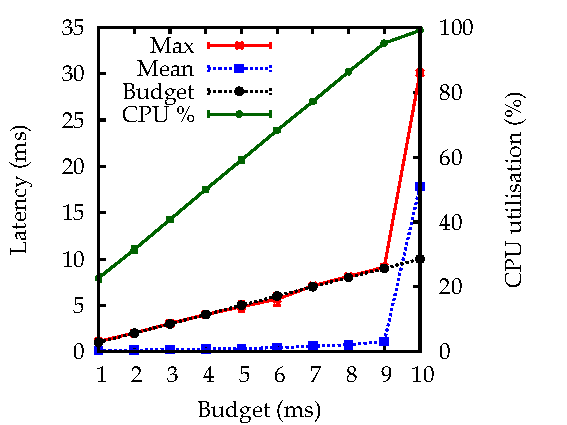
\includegraphics{ipbench}
  \caption[Results of \code{ipbench} isolation benchmark.]{Average and maximum latency of UDP packets with
  a CPU-hog VM running a high priority with a 10\,ms budget.}
  \label{f:ipbench}
\end{figure}

% Show isolation in a shared server
\subsection{Server isolation} 
\label{s:server-isolation}

To demonstrate temporal isolation in a shared server, we use a case study of an encryption service
using \gls{AES} to encrypt client data. We measure both the overhead of different
recovery techniques, and the throughput achieved when two clients constantly run out of budget in the server. 
We port an existing, open-source \gls{AES} implementation to a shared server running on \selfour, and run
benchmarks on both \textsc{x86} and \textsc{Sabre}.

\Cref{f:aes-arch} shows the architecture of the case study. Both clients $A$ and $B$ are single
 threaded and exist in separate address spaces to the server. The server has two threads, a passive
 thread for serving requests on the client's scheduling context and an active thread which handles
 timeout exceptions for the server. The server and timeout exception handler share the same virtual
 memory and capability spaces.

\begin{figure}
\centering
\includegraphics{aes-arch}
\caption[Architecture of the AES case study.]{Architecture of the \gls{AES} case study. Client $A$ and $B$ make \gls{IPC} requests over
endpoint $E_{1}$ of passive $AES$ which has an active timeout fault handling thread waiting for
fault \gls{IPC} messages on endpoint $E_{2}$.}
\label{f:aes-arch}
\end{figure}

The server itself runs the AES-256 algorithm with a block size of 16~bytes. The server alternates between two
buffers, using an atomic swap, of which one always contains consistent state, the other is
dirty during processing. When a timeout fault occurs, only the dirty buffer is lost due to
inconsistency. Both clients request 4\,MiB of data to be encrypted, provided by a shared buffer
between client and server, and have a budget insufficient to
complete the request. When the server is running on the client's scheduling context and the budget
expires, a timeout exception, which is a fault IPC message from the kernel, is delivered to the timeout
handler. 

\subsection{Timeout handling techniques}

If a client's scheduling context is depleted while the server is servicing the request, a timeout fault
is raised and sent to the timeout handler.  The appropriate protocol for handling such faults
depends ultimately on the requirements of the system.  Consequently, we implement and evaluate four
different timeout fault handling techniques: \emph{rollback}, \emph{error}, \emph{emergency} and
\emph{extend}. 

While each technique is evaluated separately, combinations of such techniques could be used for
different clients, depending on their requirements. For example, trusted clients may get special
treatment. Note that in all cases of blocking IPC, clients must trust the server as discussed in
\cref{s:locking}. Additionally, although our experiment places 
the timeout fault handler in the server's address
space, this is not necessary: for approaches that require access to scheduling contexts and
scheduling control capabilities, the timeout handler may be placed in a scheduling server's address
space, separate from the server itself.

\subsubsection{Rollback}

Rollback restores the server to the last known consistent state recorded. In the case of non-thread
safe servers, this may require rolling back an entire request. However, algorithms like \gls{AES}
which can easily be batched can make progress. The process for rollback is as follows:

\begin{enumerate}\label{e:rollback}
    \item A timeout fault is received by timeout handler, $T$ over $E_{2}$.
    \item $T$ constructs a reply message to the client from the last clean state, and sends this 
        message to the client by invoking the resume capability that the server has used for that client. 
        Because the resume object tracks the donation, the client's scheduling context is returned.
    \item $T$ then restores the server, $S$, to a known state (restoring registers,
        stack frames and any global state). $S$ is restored to the point before it made its
        last system call, usually an \nbsendrecv, which it used to indicate to the initialiser that
        $S$ should be made passive, as part of the passive server initialisation protocol presented
        in \cref{sec:impl-passive-servers}.
    \item Now the server must return to blocking on the IPC endpoint, $E_{1}$. $T$ binds a
        scheduling context to $S$ and waits for a message. 
    \item Now the $S$ runs from its checkpoint, repeating the \nbsendrecv, signalling to $T$ that it
        can now be converted to passive once more and blocking on $E_{1}$. 
    \item $T$ wakes and converts the server back to passive.
    \item Finally, $T$ blocks on $E_{2}$, ready for further timeout faults.
\end{enumerate}

The rollback technique requires the server and timeout handler to both have access to the reply
object that the server is using, and the server's \gls{TCB}, meaning the timeout handler must be
trusted by the server. In our example the server and timeout handler run at the same priority, in
all cases both must run at higher priorities than the clients, to allow the timeout handler to
reinitialise the server in the correct order, and to implement the \gls{IPCP}. 

Once the budget of the faulting client is replenished, it can then continue the request based on the
content of the reply message sent by the timeout handler. Clients are guaranteed progress as long as
their budget is sufficient to complete a single batch of data.

If rollback is not suitable, the server can be similarly reset to the initial state and an error
returned to the client. However, this does not guarantee progress for clients with insufficient
budgets.

\subsubsection{Kill}

In cases of non-preemptible servers, potentially due to a lack of thread safety, one option is to
kill client threads. Such a scenario would stop untrusted misbehaving clients from constantly
monopolising server time.  We implement an example where the timeout handler has access to client \gls{TCB}
capabilities and simply calls suspend, however the server could also switch to a new reply object
and leave the client blocked forever, without access to any of the clients capabilities. 

The process for suspending the client is the same as that for \Cref{e:rollback} but for two aspects;
the server state does not need to be altered by the timeout handler as the server always 
restores to the same place, instead of replying to the client it is suspended.

\subsubsection{Emergency}

Another technique gives the server a one-off emergency budget to finish the client request, after
which the exception handler resets the server to being passive. This could be used in low
criticality \gls{SRT}
scenarios where isolation is desired but transient overruns are expected.
An example emergency protocol follows:

\begin{enumerate}\label{e:emergency}
    \item A timeout fault is received by timeout handler, $T$ over $E_{2}$.
    \item $T$ unbinds the client scheduling context from $S$.
    \item $T$ binds a new scheduling context to $S$, which acts as an emergency budget.
    \item $T$ then replies to the timeout fault, resuming $S$.
    \item Now $T$ enqueues itself on $E_{1}$, such that when the server finishes the blocked request,
        $T$, being a higher priority, is served next.
    \item $S$ completes the request and replies to the client.
    \item $S$ receives the request from $T$, and replies immediate as it is an empty request.
    \item $T$ wakes, and converts the server back to passive.
    \item Finally $T$ blocks on $E_{2}$, ready for further timeout faults.
\end{enumerate}

This case requires the timeout handler to have access to clients' scheduling contexts, in order to
unbind them from the server. 

\subsubsection{Extend}

The final technique is to simply increase the client's budget on each timeout, which requires the
timeout fault handler to have access to the client's scheduling contexts.
This could be deployed in \gls{SRT} systems or for specific threads with unknown budgets up to a limit. 

\begin{enumerate}\label{e:extend}
    \item A timeout fault is received by timeout handler, $T$ over $E_{2}$.
    \item $T$ extends the client's budget by configuring scheduling context.
    \item $T$ replies to the fault message, which resumes $S$.
\end{enumerate}

%\newpage
\begin{table}[t!]\centering
\begin{tabular}{cllrrrr}\toprule
\emph{Platform} & \emph{Operation} & \emph{Cache} & \emph{Min} &
                          \emph{Max} & \emph{Mean} &
                          \multicolumn{1}{c}{\boldmath \(\sigma\)} \\\midrule
                          \multirow{8}{*}{\textsc{x64}}
                          \input{data/generated/haswell-aes.inc}
                          \midrule
                          \multirow{8}{*}{\textsc{Sabre}} 
                          \input{data/generated/sabre-aes.inc} 
                          \midrule
                          \multirow{8}{*}{\textsc{HiKey64}} 
                          \input{data/generated/hikey64-aes.inc} 
                          \midrule
                          \multirow{8}{*}{\textsc{TX1}} 
                          \input{data/generated/tx1-aes.inc} 
                          \bottomrule
\end{tabular}
\caption[Cost of timeout handler operations.]{Cost of timeout handler operations in \(\mu\)s, as measured
  by timeout exception handler. \(\sigma\) is the standard deviation.}
\label{t:rollback}
\end{table}


\subsection{Results}

We measure the pure handling overhead in each case, from when the timeout handler wakes up to when
it blocks again.  Given the small amount of rollback state, this measures the baseline overhead. For
schedulability analysis, the actual cost of the rollback would have to be added, in addition to the
duration of the timeout fault IPC. 
 
We run each benchmark with hot caches (primed by some warm-up
iterations)  as well as cold (flushed) caches and measure the 
latency of timeout handling, from the time the handler wakes up
until it replies to the server.

\autoref{t:rollback} shows the results. The maximum
cold-cache cost, which is relevant for schedulability analysis, differs by a factor of 3--4 between
the different recovery scenarios, indicating that all are about equally feasible.  Approaches that
restart the server and send \glspl{IPC} messages on its behalf (rollback, reply) are the most
expensive as they must restore the server state from a checkpoint and follow the passive server
initialisation protocol (recall \cref{sec:impl-passive-servers}). 

\subsection{Rollback isolation}

\begin{figure}[t]
  \centering
  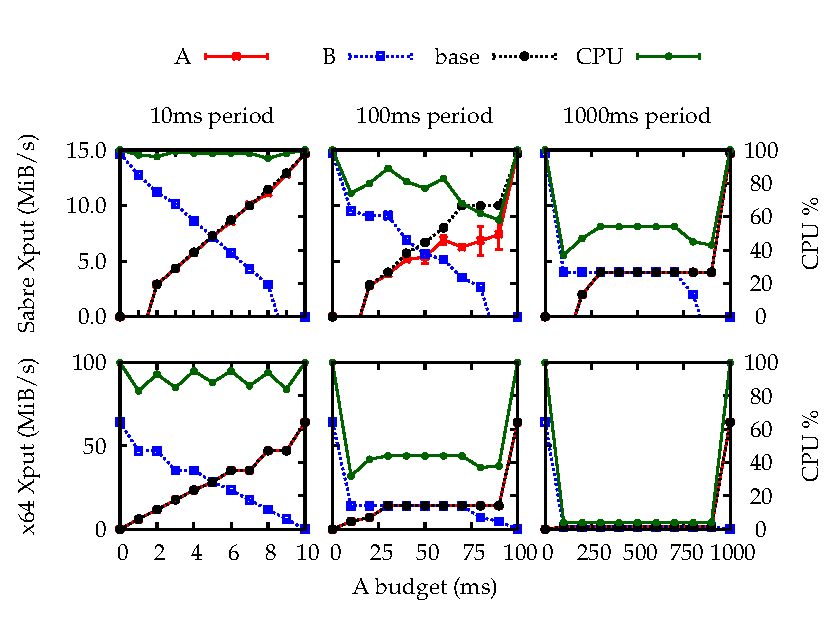
\includegraphics{aes-shared}
  \caption[Results of AES server isolation benchmark.]{Throughput for clients A and B of a passive AES server processing 10 requests of 4\,MiB of data with
      limited budgets on the \textsc{x64} (top row) and \textsc{Sabre} (bottom row) platforms. The two clients' budgets
      add up to the period, which is varied between graphs (10, 100, 1000\,ms). Clients sleep when
      they process each 4\,MiB, until the next period, except when their budgets are full. Each data point is the average of 10 runs, error bars show the standard deviation.}
  \label{f:aes}
\end{figure}

We next demonstrate temporal isolation in the server by using the rollback
technique and measuring the time taken to encrypt 10 requests of 4\,MiB of
data. \autoref{f:aes} shows the result with both clients having the same
period, which we vary between 10\,ms and 1000\,ms.
In each graph we vary the clients' budgets between 0 and the
period. The extreme ends are special, as one of the clients has a full
budget and keeps invoking the server without ever getting rolled back,
thus monopolising the processor. In all other cases, each client
processes at most 4\,MiB of data per period, and either succeeds (if
the budget is sufficient) or is rolled back after processing less than 4\,MiB.

The results show that in the CPU-limited cases (left graphs)
we have the expected near perfect proportionality between throughput and
budget (with slight wiggles due to the rollbacks), showing isolation between clients. In the cases where there is headspace (centre of the right
graphs), both clients achieve their desired throughput.

\section{Practicality}

Fundamental to the microkernel philosophy is keeping policy out of the
kernel as much as possible, and instead providing general mechanisms
that allow the implementation of arbitrary policies
\citep{Heiser_Elphinstone_16}.  On the face of it, our
fixed-priority-based model seems to violate this principle, but we
demonstrate that the model is general enough to support the efficient
implementation of alternate policies at user level. Specifically, we
implement two user-level schedulers: first, a static mixed criticality
scheduler~\citep{Baruah_BD_11}, which we also compare to an in-kernel
implementation, and an \gls{EDF} scheduler, which we compare to \litmus.

\subsection{Criticality}

\begin{figure}[t]
  \centering
  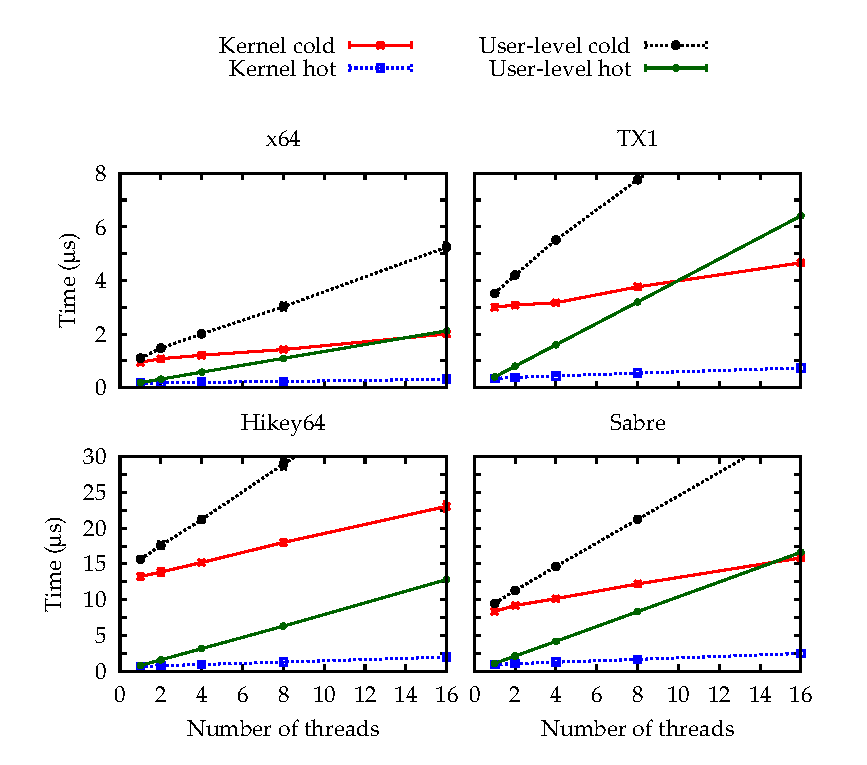
\includegraphics[width=\textwidth]{mode-switch-all}
  \caption[Kernel vs. user-level criticality switch.]{Cost of switching the priority of $n$ threads in kernel and user level, with hot
      and cold caches, on \textsc{x64} (top-left), \textsc{TX1} (top-right), \textsc{HiKey64}
      (bottom-left) and \textsc{Sabre} (bottom-right). All data points are the average of 100 runs,
                  with very small standard deviations.}
  \label{f:mode-switch}
\end{figure}


Static, mixed-criticality, fixed-priority schedulers are based on \emph{mode
switches}, which effectively mean altering the priority of threads in bulk:
critical threads that may be of low rate are bumped to higher than their
low-criticality counter parts, to ensure deadlines are met in exceptional
circumstances. 

We implement a kernel mechanism for changing thread priorities in bulk,
and compare with a user-level approach which simply changes the priority of threads
one at a time. In our prototype implementation, the kernel tracks all threads of specific
criticalities and boosts their priority on a criticality switch. However, given threads are kept in per-priority queues, each thread must be removed and reinserted into a new queue, so either way the complexity of the mode-switch is $O(n)$. 

\begin{table}[t]\centering
    \rowcolors{2}{gray!25}{}
    \begin{tabular}{lrrr}\toprule
        \emph{Platform}     & \emph{Kernel cold ($\mu$s)} & \emph{User-level cold ($\mu$s)} & \emph{Diff $\mu$s} \\\midrule
        \textsc{x64}    & $\leq2$ & $\leq4$ & \textasciitilde2 \\
        \textsc{TX1}    & $\leq4$ & $\leq8$ & \textasciitilde4 \\
        \textsc{HiKey64}    & $\leq18$ & $\leq30$ & \textasciitilde12 \\
        \textsc{Sabre}    & $\leq12$ & $\leq22$ & \textasciitilde10 \\
        \bottomrule
\end{tabular}
\caption[Comparison of kernel and user-level priority switches]{Comparison of cold, in-kernel
priority switch to cold, user-level priority switch.}
\label{t:cold-prio-switch}
\end{table}


\autoref{f:mode-switch} shows the results measured with a primed cache (hot) and flushed cache (cold).
As the graph shows, switching is linear in the number of threads being boosted, in both kernel and
user-level implementations.
\Cref{t:cold-prio-switch} compares the results of cold, in-kernel switching to user-level in roughly
absolute terms. \textsc{HiKey64} is the slowest at 30\,\(\mu\)s with eight threads to switch,
due to the smaller L2 cache and
in-order execution, however all platforms show roughly the same factor of two increase when
comparing kernel and user-level cold-cache results.
However, most systems will not have more than a few high-criticality threads, and deadlines for critical control loops in
cyber-physical systems tend to be in the tens of milliseconds, we
conclude that criticality can be implemented at user-level, in line with standard microkernel philosophy.

The higher cost from user-level operation results from  multiple
switches between kernel and user mode, and the repeated
thread-capability look-ups. It could be significantly reduced if seL4
had a way to batch system calls, but to date we have seen no compelling use cases for this.

As a second criticality-switch benchmark, we ported three processor intensive 
benchmarks from the MiBench~\citep{Guthaus_REAMB_01} to act as workloads. 
We use \textsc{susan}, which performs image recognition, \textsc{jpeg}, which does image
encoding/decoding, and \textsc{mad}, which plays an MP3 file.
Each benchmark runs in its own Rump process
with an in-memory file system, and shares a timer and serial server.
 We chose these specific
benchmarks as they were the easiest to adapt as described below, and use them as workloads,
rather than for comparing systems, so there is no issue of bias from sub-setting.

We alter the benchmarks to run periodically in multiple stages. To obtain
execution times long enough, some benchmarks iterate a fixed number of times per
stage. Each benchmark process executes its workload and then waits for the next period to start.
Deadlines are implicit: if a periodic job finishes before the start of the next period, it is
considered successful, otherwise the deadline is missed.

We run the benchmarks on both the user-level and in-kernel implementations of static mixed criticality, with 10 runs of each.

\begin{table}[t]
    \centering
    \begin{tabular}{lcccccclcl}\toprule
        \emph{Application} & \emph{T} & \emph{L} & \emph{\(L_S\)} & \emph{C} & \emph{U} & \emph{j} &
        & \emph{m}  & \\\midrule
        \input{data/generated/mode_switch.inc}
        \bottomrule
    \end{tabular}
    \caption[Results of criticality switch benchmark.]{Results of criticality switch benchmark for each
        stage, where the  criticality \(L_S\) is raised each stage. \(T\) =
        period, \textit{C} = worst observed execution time (ms),
      \textit{U} = allowed utilisation (budget/period),
      \textit{m} = deadline misses, \textit{j} = jobs completed. We record 52 (0.1), 86 (15.2)
      and 100 (0.0)\% CPU
utilisation for each stage respectively. Standard deviations are shown in parentheses. Bold values
show the difference between the user-level scheduler and kernel. }
    \label{t:modeswitch}
\end{table}


Results are shown in \autoref{t:modeswitch}. For both schedulers (kernel versus user-level), 
the results are nearly exactly the same. Bold numbers indicate a difference between the kernel and
user-level scheduler, with only the lowest-criticality thread affected by the criticality switch, with an additional missed deadline due to
perturbations in run time due to the slightly slower user-level scheduler.
For stage one, the entire workload is schedulable and
there are no deadline misses. For stage two, the workload is not
schedulable, and the criticality switch boosts the priorities of
\textsc{susan} and \textsc{jpeg}, such that they meet
their deadlines, but
\textsc{mad} does not. In the final stage, only the most critical task
meets all deadlines.
This shows that it is sufficient to implement criticality at user-level, and our mechanisms operate as intended.

\subsection{User-level EDF}\label{s:edf-impl}

\begin{listing}
\inputminted{c}{code/edf.c}
\caption{Pseudocode for the EDF scheduler.}
\label{list:edf}
\end{listing}

We implement the EDF scheduler as an active server with active
clients which run at an \selfour priority below the user-level scheduler.
The scheduler waits on an endpoint on which it receives messages from
its clients and the timer, as shown in \cref{list:edf}.

Each client has a period, representing its relative deadline, and a full reservation (equal to the period). Clients
either notify the scheduler of completion by an IPC
message, or else create a timeout exception on preemption, which is also received by the
scheduler. Either is an indication that the next thread should be scheduled.

\begin{figure}[t]
\centering
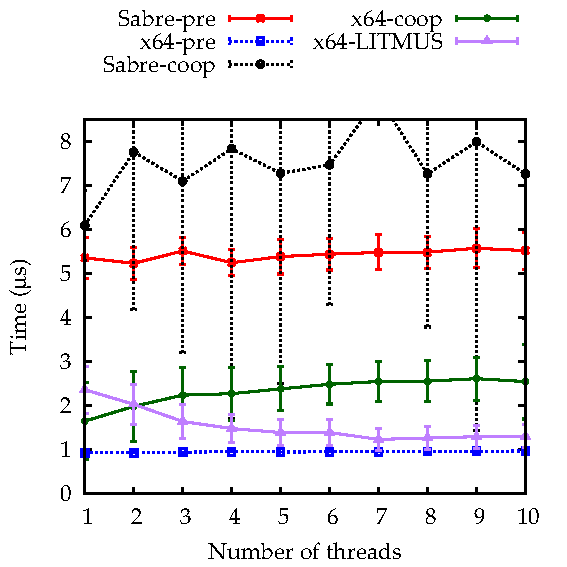
\includegraphics{edf}
\caption[Results of \selfour user-level EDF versus \litmus.]{Execution time of \selfour user-mode EDF scheduler compared to
         kernel scheduler in \textsc{x64} \litmus.}
\label{f:edf}
\end{figure}


We use the \emph{randfixedsum}~\citep{Emberson_SD_10} algorithm with periods ranging from 10-1000ms
(log-uniform distribution) and implicit deadlines. 
A set of threads runs until 100
scheduling decisions have been recorded. We repeat this 10 times,
resulting in 1,000 scheduler runs for each data point.

We measure the scheduler latency by recording the timestamp when each client thread, and an idle
thread, detects a
context switch and processing the difference in timestamp pairs offline. We run two schedulers:
\emph{pre}-empt where threads never yield and must incur a timeout exception, and \emph{coop}, where
threads use IPC to yield to the scheduler. The latter invokes the user-level timer
driver more often as the release queue is nearly always full, which involves more kernel invocations
to acknowledge the IRQ, in addition to reprogramming the timer.

We compare our latencies to those of
LITMUS$^{RT}$~\citep{Calandrino_LBDA_06}, a widely-used real-time scheduling
framework for developing real-time schedulers and locking protocols. 
As it is  embedded in Linux, LITMUS$^{RT}$ is not aimed at high-assurance systems.

We use Feather-Trace~\citep{Brandenburg_Anderson_07} to gather data.
We use the C-EDF scheduler, which is a partitioned (per-core) EDF scheduler, on a single
core. We use the same parameters and thread sets, running each set for 10\,s. 
The measured overhead considers the in-kernel scheduler, context-switch and user-level code to return to
the user.

\autoref{f:edf} shows that our preemptive user-level EDF scheduler implementation is
actually faster than the in-kernel EDF scheduler from LITMUS$^{RT}$, and
that the cost of implementing scheduling policy at user level of time-triggered systems is of
the same order as the in-kernel default scheduler. In other words,
implementing different policies on top of the base scheduler is quite feasible.

The benchmark is by no means a worst-case overhead and actually shows a favourable overhead for both
platforms as neither task set exercised the cache. Due to seL4's much smaller cache footprint than
Linux, it is likely seL4 would be more competitive if tasks had a significant cache footprint. Also
note that as the C-EDF scheduler contains locking primitives for managing multiple cores, the LITMUS
overheads are higher than they would be if a uniprocessor scheduler (PSN-EDF) was used for the
benchmark.

\section{Multiprocessor benchmarks}

We run two multicore benchmarks, the first evaluating multicore throughput of the MCS kernel versus the
baseline kernel, the second based on our shared server \gls{AES} case study to demonstrate the
multicore model. 

We run multiprocessor benchmarks on two of our platforms, \textsc{Sabre} and \textsc{x64}. Both 
are symmetric multiprocessors with four cores. 

\begin{figure}[t] 
    \centering
    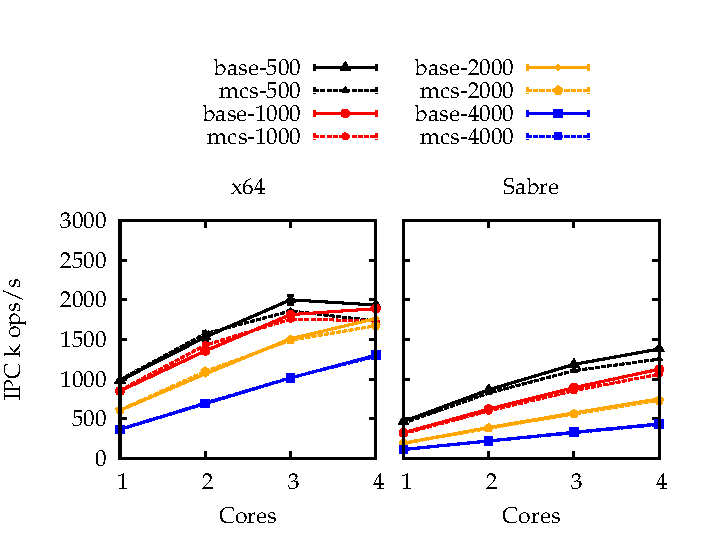
\includegraphics{smp}
    \caption[Results of the multicore IPC throughput benchmark.]{Results of the multicore IPC throughput benchmark, baseline \selfour vs MCS. 
        Each series is named \textit{name-N}, where \textit{name} is \textit{base} and \textit{mcs} for 
        the baseline and MCS kernel respectively, and \textit{N} is the upper
        bound on the number of cycles between each IPC for that series.}
    \label{f:evaluation-smp}
\end{figure}

\subsection{Throughput}

We run a multicore throughput benchmark to show that our MCS model
avoids introducing scalability problems on multiple cores compared to the baseline kernel.
We modify the
existing multicore IPC throughput benchmark for \selfour to run on the MCS kernel. 
At time of writing, only \textsc{x64} and \textsc{sabre} have \selfour multiprocessor support, 
consequently these are the platforms used for the benchmark.

The existing multicore benchmark measures IPC throughput of a client and server, both 
pinned to the same processor, sending fastpath, 0-length IPC messages via \call
and \replyrecv. One pair of client and server is set up per core. Both threads are
the same priority and the messages are 0 length. Each thread spins for a random amount
with an upper bound \textit{N} between each subsequent IPC. As \textit{N} increases so does
IPC throughput, as fewer calls are made.

We modify the benchmark such that each server thread is passive on the MCS kernel.
Results are displayed in \Cref{f:evaluation-smp} and show a minor impact on IPC throughput
for low values of \textit{N}. Scalability is not impacted on \textsc{sabre}, but is on \textsc{x64},
with the curve flattening slightly more aggressively on the MCS kernel
due to the fastpath overhead. The low overhead is expected as the MCS model only introduces extra 
per-core state, with no extra shared state between cores. The slight scalability impact is
due to a higher cache-footprint of the IPC fastpath. 
\clearpage
\subsection{Shared server}

\begin{figure}[t] 
    \centering
    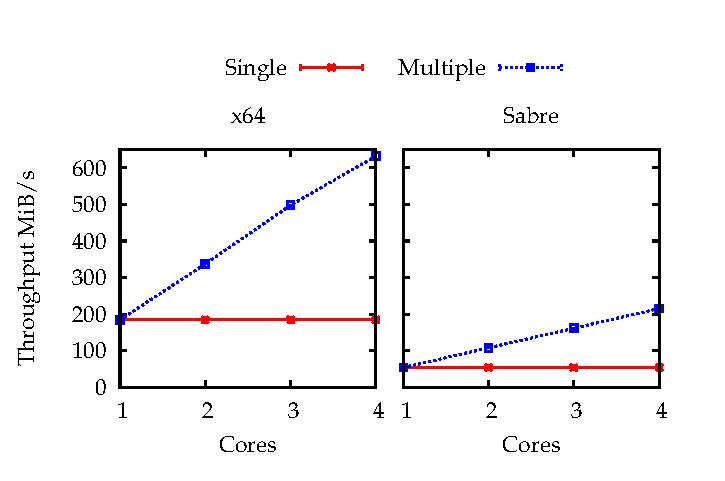
\includegraphics{smp_aes}
    \caption[Results of the AES shared server multicore case study.]{Results of the AES shared server multicore case study. \emph{Single} shows results for a 
        passive server thread migrating between cores to service clients, while \emph{Multiple} has one
        passive server thread per core. For both series, the number of clients is equal to the number of
        cores and each client requests 1MiB of data encrypted. }
    \label{f:evaluation-smp-aes}
\end{figure}

We adapt our \gls{AES} case study (\cref{s:server-isolation}) to demonstrate how our MCS model 
applies to multiprocessors. The AES server is configured without a timeout fault handler, and
we run two variants. 

\begin{description}
    \item[Single:] the AES server has a single passive thread, which waits on a single endpoint
        and migrates to the core of the active client over IPC, effectively serialising access to the server.
        Consequently, \cref{f:evaluation-smp-aes} shows there is no gain in throughput when further cores are
        added. 
    \item[Multiple:] the AES server has one passive thread per core, and an endpoint is set up for
        each core, demonstrating a parallel server. Due to the absence of bottlenecks in the stateless 
        AES server, this results in near perfect scalability.
\end{description}

\section{Summary}

All in all, we have demonstrated via micro- and macro- benchmarks that our overheads are
reasonable given the speed of the baseline kernel and the extent of the provided
functionality. 

Through two system benchmarks and one shared-server benchmark, we have shown
that our approach guarantees processor isolation and that threads cannot exceed
their budget allocation via their scheduling context. Additionally, we have
shown that isolation can be achieved in a shared server via a timeout-fault
handler, and implemented several alternatives for handling such faults,
demonstrating the feasibility of the model. 

Policy freedom is maintained despite providing fixed-priority scheduling in the kernel, as the
mechanisms are sufficient to implement low-overhead, user-level schedulers, 
as demonstrated through the static, mixed-criticality and EDF scheduler
implementations. 

Finally, we have demonstrated that the model works for multiprocessors,
incurring no great scalability penalty over baseline \selfour, 
and show how passive servers migrate across cores on \gls{IPC}.

\chapter{Conclusion}
\label{chap:conclusion}

Emerging cyber-physical systems represent an opportunity for greater safety, security and 
automation, as they can replace systems where human errors prevail. While humans are excellent at
innovation and creativity, they cannot compete with machines that do not get tired, drunk or
distracted when completing
monotonous, repetitive tasks. Car accidents are overwhelmingly 
caused by human error, measured at 94\% in the US~\citep{Singh_15}, something that self-driving cars can overcome. Autonomous aircraft and other fleet vehicles, smart cities and smart factories hold similar promise. 

As established in \cref{sec:motivation}, in order to practically develop such systems,
they must be mixed-criticality, as certification of all parts of such a system to high-assurance
levels is not feasible. Consequently, mixed-criticality systems require strong temporal isolation
and asymmetric protection between sub-systems of different criticality levels, 
which must also be able to safely share resources.

This thesis has drawn on real-time theory and systems practice to develop core mechanisms required
in a high-assurance, trusted computing base for mixed criticality systems. Importantly, the
mechanisms we have developed do not violate other requirements, like policy-freedom, integrity,
confidentiality, spatial isolation, and security. 

In \cref{chap:model}, we introduced our model for treating time as a first-class resource, and 
defined a minimal set of
mechanisms that can be leveraged to implement temporal isolation between threads, even within shared
servers. Our primitives also allow for more complex, application-specific user-level schedulers to
be constructed efficiently, as we demonstrated in the evaluation. Significantly, we provide a
new model for L4 kernels to manage time as a first-class resource, without restricting policy
options including overbooking, 
or requiring specific correlations between the priority of a task and the scheduling model, or
importance of that task. 
We integrate a capability system with the non-fungible resource that is time, without violating our
existing isolation and confidentiality properties, or requiring a heavy performance overhead.
Our mechanisms provide a basic scheduler, which is a critical part of the
trusted computing base, and allow for more system-specific schedulers to be constructed at
user-level. Additionally, we do not force specific
resource-sharing prioritisation policies, but provide mechanisms to allow for their implementation at user-level. 
\clearpage

\section{Contributions}

Specifically, we make the following contributions:

\begin{itemize}
    \item Mechanisms for principled management of time through capabilities to scheduling contexts,
        which are compatible with the fast IPC implementations traditionally used in high-performance
        microkernels, and also compatible with established real-time resource-sharing policies;
    \item an implementation of those mechanisms in the non-preemptible \selfour microkernel, and an
        exploration of how the implementation interacts with the existing kernel model;
    \item an evaluation of the overheads and isolation properties of the implementation, including
        a demonstration of isolation in a shared server through timeout-fault handling;
    \item a design and implementation of many different, user-level timeout-fault handling policies;
    \item and an implementation of a user-level \gls{EDF} scheduler which is as fast as the
        \litmus in-kernel EDF scheduler, which shows that despite the fixed-priority scheduler
        present in the kernel, other schedulers remain practical;
    \item and a design and implementation of a criticality switch at user-level, which shows that
        criticality is not required to be a kernel-provided property.
\end{itemize}

The implementation is complete, and the verification of this implementation is currently in progress.
Specifications have already been developed by the verification engineering team at Data61, CSIRO,
who are now completing the first-level refinement of the functional correctness proof.
The maximum controlled priority feature has already been verified and merged to the master kernel. 
Verification is beyond the scope of this PhD, although we continue to work closely with
the team to assist in verification. 

This work is part of
the Side-Channel Causal Analysis for Design of Cyber-Physical Security project for the U.S
Department of Homeland Security.

Additionally, during the development of this thesis we have made extensive contributions to the 
\selfour benchmarking suite, testing suite and user-level libraries, all of which provide better 
support for running experiments and building systems on \selfour. 

\section{Future work}

Modern \glspl{CPU} have dynamic frequency scaling and low-power modes in order to reduce energy usage, which
is of high concern in many embedded systems. The implementation as it stands assumes a constant
\gls{CPU} frequency, and all kernel operations are calculated in \gls{CPU} cycles. Frequency scaling
can have undesirable effects on real-time processes: if the period is specified in microseconds, then
converted to cycles and the CPU frequency changes, does the period remain correct? This is a
limitation of our model and promising area for future work.

Although we provide a mechanism for cross-core IPC, where passive threads migrate between processing
cores and active threads remain fixed, there is much more to consider in terms of multicore
scheduling and resource sharing. Our model provides a partitioned, fixed priority scheduler, and 
load balancing can be managed by user level. Further experiments to evaluate the mechanisms for higher-level
multicore scheduling and resource sharing protocols is required. 

Finally, this work does not consider counter-measures for timing-related covert and side channels,
security risks which arise from
shared hardware~\citep{Ge_YCH_18}. \emph{Covert channels} are unintentional, explicit communication
channels which may be used by a malicious sender in a trusted component to leak sensitive data to a receiver
in an untrusted component. Providing a time-source can open a covert channel, where the sender
manipulates timing behaviour through shared architectural structures like caches, and the receiver
uses the time source to observe the behaviour. Shared hardware also presents the risk of
\emph{side channels}, 
where an attacker in an untrusted
component can learn secret information about a trusted component by observing timing behaviour. 
Both attack vectors are risks in mixed-criticality systems, which we do not consider in this
thesis, and merit extensive future work. 

\section{Concluding Remarks}

Original automobiles did not have seat belts, as safety was never a concern. Perhaps one day we
will reflect on human-piloted, high-speed vehicles in the same way. For this future to eventuate, 
cyber-physical systems which combine components of different criticality on shared hardware are essential.
Our work has focused on principled mechanisms for managing time in such systems,
making one significant step towards a future of trustworthy,
safe and secure autonomous systems.

\bigskip
This material is based on research sponsored by the Department of Homeland Security (DHS) Science
and Technology Directorate, Cyber Security Division (DHS S\&T/CSD) BAA HSHQDC-14-R-B00016, and the
Government of United Kingdom of Great Britain and the Government of Canada via contract number
D15PC00223. 

%{
%\backmatter - back matter screws up numbering for appendixes so don't use it
\cleardoublepage
\bibliographystyle{plainnat}
\bibliography{references}

%}
\appendix
\appendixpage
\input{api.tex}
\chapter{Fastpath Performance}
\input{data/generated/kzm-ipc-perf.inc}
\input{data/generated/sabre-ipc-perf.inc}
\input{data/generated/hikey32-ipc-perf.inc}
\input{data/generated/hikey64-ipc-perf.inc}
\input{data/generated/tx1-ipc-perf.inc}
\input{data/generated/haswell-ipc-perf.inc}
\end{document}
